\documentclass[doctor]{iscs-thesis}

\usepackage{amsmath, stmaryrd, rotating, amssymb,
setspace, float, amsthm}
\usepackage{bussproofs}

%%% from master thesis

\usepackage{rotating}

\usepackage{bussproofs,stmaryrd, amssymb, amsmath, amsthm, showlabels}
\newcommand{\ruleT}[1]{\LeftLabel{(T)}\UnaryInfC{${#1}$}}
\newcommand{\powerset}[1]{{\mathcal P({#1})}}
\newcommand{\proj}[0]{\operatorname{proj}}
\newcommand{\len}[0]{\operatorname{len}}
\newcommand{\cl}[0]{\operatorname{cl}}
\newcommand{\carrier}[0]{\operatorname{carrier}}
\newcommand{\subfml}{\operatorname{subfml}}
\newcommand{\seq}{\operatorname{Seq}}
\newcommand{\type}{\operatorname{Type}}
\newcommand{\vdashsc}{\vdash_{\mbox{\rm sc}}}
\newcommand{\iec}{{\rm {\textbf{IEC}}}}
\newcommand{\ckv}{{\rm {\textbf{S4}\ast\cdots\ast\textbf{S4}}}}
\newcommand{\vdashsf}{\vdash_{\ckv}}
\newcommand{\initial}[1]{${#1}\vdashn{#1}$}
\newcommand{\supsete}[1]{\LeftLabel{($\supset$-E)}\BinaryInfC{${#1}$}}
\newcommand{\supseti}[1]{\LeftLabel{($\supset$-I)}\UnaryInfC{${#1}$}}
\newcommand{\nec}[1]{\LeftLabel{(nec)}\UnaryInfC{${#1}$}}
\newcommand{\wedgeel}[1]{\LeftLabel{($\wedge$-E$_0$)}\UnaryInfC{${#1}$}}
\newcommand{\wedgei}[1]{\LeftLabel{($\wedge$-I)}\BinaryInfC{${#1}$}}
\newcommand{\veeil}[1]{\LeftLabel{($\vee$-I$_0$)}\UnaryInfC{${#1}$}}
\newcommand{\veeir}[1]{\LeftLabel{($\vee$-I$_1$)}\UnaryInfC{${#1}$}}
\newcommand{\veee}[1]{\LeftLabel{($\vee$-E)}\TrinaryInfC{${#1}$}}
\newcommand{\weaken}[1]{\LeftLabel{(w)}\UnaryInfC{${#1}$}}
\newcommand{\be}[1]{\LeftLabel{($\bot$-E)}\UnaryInfC{${#1}$}}
\newcommand{\ax}[1]{	     \AxiomC{}
	     \LeftLabel{(ax)}
\UnaryInfC{\initial{#1}}}
\newcommand{\dn}[1]{\LeftLabel{(DN)}\UnaryInfC{${#1}$}}

\newenvironment{example}[1][Example]{\begin{trivlist}
    \item[\hskip \labelsep {\bfseries #1}]}{\end{trivlist}}
\newenvironment{remark}[1][Remark]{\begin{trivlist}
    \item[\hskip \labelsep {\bfseries #1}]}{\end{trivlist}}

\usepackage{graphicx}	% required for `\includegraphics' (yatex added)
\usepackage[numbers,sort&compress]{natbib}

%%% end from master thesis

%%% from haskell symposium submitted paper
\usepackage{graphicx}
\usepackage{bussproofs}
\usepackage{amsmath,amssymb}
%\usepackage{showlabels}

\usepackage{setspace}

%\doublespacing

\newcommand{\Nat}{{\mathbb N}}
\newcommand{\Real}{{\mathbb R}}
\newcommand{\pvar}{\mathcal V_P}
\newcommand{\agents}{\mathcal A}
\newcommand{\wvar}{\mathcal V_W}

\newcommand{\tuple}[1]{\langle{#1}\rangle}
\newcommand{\fix}[1]{[FIX \fbox{#1}]}
\newcommand{\fml}{\operatorname{Fml}}
\newcommand{\id}{\operatorname{id}}
\newcommand{\kv}{$\mathbf K \vee$}
\newcommand{\vdashR}{\vdash_{\mathsf R}}

\newcommand{\vdashRLB}{\vdashR^{\mbox{\tiny \LB}}}

\newcommand{\T}{\mathbf T}
\newcommand{\memory}{{\sf m}}
\newcommand{\ruleskip}{\vskip 5mm}

%%% 

\newcommand{\R}[1]{{#1}^{\mathsf R}}
\newcommand{\modelsR}{\models_{\mathsf R}}


\newtheorem{notation}{Notation}
\newtheorem{proposition}{Proposition}
\newtheorem{definition}{Definition}
\newtheorem{lemma}{Lemma}
\newtheorem{corollary}{Corollary}
\newtheorem{theorem}{Theorem}



\newcommand{\nat}{\mathbb{N}}
\newcommand{\steps}[2]{Steps_{#1}\left({#2}\right)}

\newcommand{\hypc}[2]{{\mathcal{C}#1}\left[{#2}\right]}
\newcommand{\hyper}{\mathcal{H}}
\newcommand{\hypert}{\mathcal{O}}
\newcommand{\hmid}{\mid\mid\mid}

\newcommand{\tr}{\vartriangleright}
\newcommand{\update}{\vartriangleleft}

\newcommand{\elim}{\mathcal E}
\newcommand{\intro}{\mathcal I}

\newcommand{\coml}{\leftarrow_{\mathrm g}}
\newcommand{\comr}{\leftarrow_{\mathrm d}}

\newcommand{\reduce}{\rightsquigarrow}
\newcommand{\reduction}{\reduce^\ast}
\newcommand{\processes}{\mathbb{P}}
\newcommand{\ProV}{\mathbf{ProV}}
\newcommand{\LB}{\textbf{LB}}
\newcommand{\p}[1]{\texttt{#1}}

%% terms
\newcommand{\g} [0]{\mathsf{g}}
\newcommand{\spair} [1]{\langle{#1}\rangle^{\square}}
\newcommand{\lpair} [1]{\langle{#1}\rangle}
\newcommand{\gpair} [1]{\langle{#1}\rangle^{\g}}
\newcommand{\cotuple}[1]{[{#1}]}
\newcommand{\ev}[1]{\mathsf{ev}\left({#1}\right)}

\newcommand{\ginl}[1]{\mathsf{inl}^{\g}\left({#1}\right)}
\newcommand{\linl}[1]{\mathsf{inl}\left({#1}\right)}
\newcommand{\sinl}[1]{\mathsf{inl}^{\square}\left({#1}\right)}
\newcommand{\bsinl}[1]{\mathsf{inl}^{\blacksquare}\left({#1}\right)}

\newcommand{\ginr}[1]{\mathsf{inr}^{\g}\left({#1}\right)}
\newcommand{\linr}[1]{\mathsf{inr}\left({#1}\right)}
\newcommand{\sinr}[1]{\mathsf{inr}^{\square}\left({#1}\right)}
\newcommand{\bsinr}[1]{\mathsf{inr}^{\blacksquare}\left({#1}\right)}

\newcommand{\gpil}[1]{\pi^{\g}_{\mathrm l}\left({#1}\right)}
\newcommand{\lpil}[1]{\pi_{\mathrm l}\left({#1}\right)}
\newcommand{\spil}[1]{\pi^{\square}_{\mathrm l}\left({#1}\right)}

\newcommand{\gpir}[1]{\pi^{\g}_{\mathrm r}\left({#1}\right)}
\newcommand{\lpir}[1]{\pi_{\mathrm r}\left({#1}\right)}
\newcommand{\spir}[1]{\pi^{\square}_{\mathrm r}\left({#1}\right)}

\newcommand{\vg}[2]{{#1}_{#2, \mathrm g}}
\newcommand{\vd}[2]{{#1}_{#2, \mathrm d}}


\newcommand{\gmat}[5]{\mathsf{match}^{\g}\,{#1}\,\mathsf{of}\, \ginl{#2}. {#3}/
\ginr{#4}. {#5}}
\newcommand{\lmat}[5]{\mathsf{match}\,{#1}\,\mathsf{of}\, \linl{#2}. {#3}/
\linr{#4}. {#5}}
\newcommand{\smat}[5]{\mathsf{match}^{\square}\,{#1}\,\mathsf{of}\, \sinl{#2}. {#3}/
\sinr{#4}. {#5}}
\newcommand{\bsmat}[5]{\mathsf{match}^{\blacksquare}\,{#1}\,\mathsf{of}\, \bsinl{#2}. {#3}/
\bsinr{#4}. {#5}}

\newcommand{\ifte}[3]{\mathsf{If}\, {#1}\, \mathsf{then}\, {#2}\, \mathsf{else}\, {#3}}

\newcommand{\ltor}[4]{\overrightarrow{{#2}^{#1}_{#3}} \left({#4}\right)}
\newcommand{\rtol}[4]{\overleftarrow{{#2}^{#1}_{#3}} \left({#4}\right)}
\newcommand{\abort}{\mathsf{abort\,}}

\newcommand{\compare}[2]{{#1} == {#2}}

\newcommand{\term} [0]{\mathcal{T}}
\newcommand{\lterm}[0]{\mathcal{T}^-}
\newcommand{\val}  [0]{\mathcal{V}}
\newcommand{\lval} [0]{\mathcal{V}^-}
\newcommand{\tj}   [2]{ {#1} \colon{#2} }

\newcommand{\wor}{\mathsf{{or}}}

\newcommand{\Id}{\mathsf{Id}}
\newcommand{\lgd}{$\lambda$-GD}

%% configuration
\newcommand{\lstore}{{\sigma}}
\newcommand{\rstore}{{\tau}}
\newcommand{\conf}[3]{(\lstore{#1},\rstore{#2},{#3})}
\newcommand{\confwithcontext}[3]{\conf{#1}{#2}{\hypert\hmid C[{{#3}}]\hmid\hypert'}}
\newcommand{\concreteconf}[3]{({#1},{#2},{#3})}

%% reductions and the like
\newcommand{\breduce}{\reduce_{\mathrm B}}
\newcommand{\areduce}{\reduce_{\mathrm A}}
\newcommand{\wreduce}{\reduce_{\mathrm W}}
\newcommand{\rreduce}{\reduce_{\mathrm R}}
\newcommand{\preduce}{\reduce_{\mathrm P}}
\newcommand{\bpreduce}{\reduce_{\mathrm{B/P}}}

%% logical rules
\newcommand{\UnaryRule}[3]{ \AxiomC{#1}
\LeftLabel{#2}
\UnaryInfC{#3} \DisplayProof} 
\newcommand{\BinaryRule}[4]{ \AxiomC{#1} \AxiomC{#2}
\LeftLabel{#3}
\BinaryInfC{#4}\DisplayProof}
\newcommand{\TrinaryRule}[5]{ \AxiomC{#1} \AxiomC{#2}
\AxiomC{#3} \LeftLabel{#4}
\TrinaryInfC{#5} \DisplayProof}

%% investi
\newcommand{\inv}[1]{{#1}^{\mathsf i}}

\newcommand{\rightlocal}{\rightsquigarrow_{\beta{\mathrm l}}}
\newcommand{\rightcomm}{\rightsquigarrow_{\beta{\mathrm c}}}
\newcommand{\rightdist}{\rightsquigarrow_{\beta{\mathrm d}}}
\newcommand{\dist}[2]{[{#1}; {#2}]}

\newcommand{\interpret}[1]{\llbracket {#1} \rrbracket}

\newcommand{\process}{p}
\newcommand{\contex}[1]{\mathcal C[{#1}]}
\newcommand{\sem}[1]{\llbracket{#1}\rrbracket}
\newcommand{\semi}[1]{\llparenthesis{#1}\rrparenthesis}

\newcommand{\wwedge}{\operatorname*{\bigwedge\kern -8pt \bigwedge}}

\etitle{A Computational Interpretation of G\"odel--Dummett Logic}


\begin{document}

\paragraph{Acknowledgement.}
The work about Hyper $\lambda$ calculus is encouraged by feedbacks from
ACAN (Algebraic and
Coalgebraic
Approaches to
Non-Classical Logics Workshop) and OPLSS'11 participants,
supported by Grant-in-Aid for JSPS Fellows 23-6978,
and partly prepared during the author's stay in
ILPS, the University of Amsterdam.


Many of the contents also appear in the author's Master's Thesis \fix{cite}.

\chapter{Introduction}

We extended the Curry--Howard correspondence to G\"odel--Dummett logic.
The Curry--Howard correspondence is \fix{add}

G\"odel--Dummett logic is an intermediate logic \fix{cite} between
classical logic and intuitionistic logic.  Every theorem in
intuitionistic logic is a theorem in G\"odel--Dummet logic and every
theorem in G\"odel--Dummett logic is a theorem in classical logic.
The inclusion is strict.  The law of excluded middle
$\varphi\vee(\varphi\supset \bot)$ is not a theorem in G\"odel--Dummett
logic and $(\varphi\supset\psi)\vee(\psi\supset\varphi)$ is not a
theorem in intuitionistic logic.

Without modalities.


In terms of Kripke semantics, the axiom is sound and complete for
requiring that the models are linearly ordered.
In terms of algebraic semantics, the axiom is sound and complete for
requiring that the truth values are linearly ordered.  \fix{ is this
usage of ``truth values'' correct? }
In terms of computation, what is it?


who said logic is about temporality.
Waitfreedom is a kind of temporality appeared in computer science.
This research shows that the proof theory is not only about abstract notions of temporality, but also about concrete notions of temporality appearing in computer science.



\section{Curry--Howard Correspondence for Different Logics}

Prawitz

Pfenning

Davies--Pfenning S4 A Modal Analysis of Staged Computation
  
Curien

Hypersequent

Game

\section{Location Aware Languages}

X10


Hypersequents were born to solve proof theoretical difficulties, but we
apply hypersequents to solve distributed computational difficulties.

\section{Properties}

\chapter{Inuitionistic Epistemic Logic}

\etitle{An Intuitionistic Epistemic Logic for Asynchronous Communication}
\jtitle{$BHsF14|DL?.$N$?$a$ND>4Q<g5ACN<1O@M}(B}
\eauthor{Yoichi Hirai}
\jauthor{$BJ?0fMN0l(B}
\esupervisor{Masami Hagiya}
\jsupervisor{$BGkC+>;8J(B}
\supervisortitle{Professor} % Professor, etc.
\date{February 10, 2010}

We apply formal constructive reasoning to
 asyncyhronous communication.
After defining a general-purpose logic called
intuitionistic epistemic logic (\iec\,in
 short), 
we solve a~motivating example problem,
 characterising waitfree communication logically in response to the
 abstract simplicial topological characterisation of
 waitfree computation given by Herlihy, Shavit, Saks and Zaharoglou 
in the celebrated G\"odel Prize winning papers.

 Intuitionistic logic is originally a formalisation of a single mathematician whose
 knowledge
 increases over time.  The logic \iec\, formalises multiple agents who communicate
 asynchronously and whose knowledge increases over time.  
The logic \iec\, has a simple language: 
 it has epistemic modality but no temporal modality
 so that it is simpler than many previous logics for communication.
 We do not need temporal modality because 
we regard time as 
the partial order in the semantics of intuitionistic epistemic logic.
 Before defining the deduction system, we first extend the informal intuitionistic
 reading of logical connectives.
 Precisely, 
 we extend Brouwer--Heyting--Kolmogorov interpretation of logical connectives
 by adding one clause reagarding the additional epistemic modality~$K_a$.
 After stating the informal meaning for the modality,
 we define a deduction system and a Kripke semantics meeting this intuition.
 Soundness, strong completeness, finite
 model property, disjunction property and decidability are
 shown. 
We also investigate the relationship between \iec\,and classilcal modal logic with multple
 S4 modalities.

On top of the logic \iec, we give an axiom type that characterises
 sequential consistency for shared memory.
 The advantage of intuitionistic logic over classical logic is shown
 in an example where a set of axioms characterises 
 sequential consistency on shared memory.
 The axioms for sequential consistency are
 meaningless in classical logic while
 meaningful in intuitionistic logic.
 The axioms are similar to 
 the axiom type for prelinerilty.
 This similarity reflects the analogy 
 between sequential consistency for shared memory scheduling 
 and linearity for Kripke frames: both require antisymmetry on schedules or models.

Finally, under sequential consistency, we give soundness and completeness between
 a set of logical formulas called waitfree assertions and a set of models called 
schedule models.
 It has been found that it is undecidable whether a task is waitfreely solvable or not.
 We show that when we only view the communication requirements of tasks,
 it is decidable whether the communication is waitfreely attainable or not.

$B9=@.<g5AE*$J7A<0E*?dO@$r!$HsF14|DL?.$K1~MQ$9$k!%(B
$BD>4Q<g5ACN<1O@M}$H8F$VHFMQ$NO@M}$rDj5A$7$F$+$i!$(B
$B2ACM$rEA$($k$?$a$NNcBj$H$7$F!$(B
waitfree$B$JDL?.$rO@M}E*$KFCD'$E$1$k!%(B
$B$3$NO@M}3XE*$JFCD'$E$1$O!$%2!<%G%k>^$r<h$C$?!$(B
Herlihy$B$H(BShavit$B$H(BSaks$B$H(BZaharoglou$B$H$K$h$k!$(B
waitfree$B7W;;$NCj>]C1BN4v2?3XE*$JFCD'$E$1$K1~$($k$b$N$G$"$k!%(B

$BD>4Q<g5AO@M}$O$=$b$=$bCN<1$rA}Bg$5$;$D$E$1$k?t3X<T$r7A<02=$7$?!%(B
$BD>4Q<g5ACN<1O@M}$O!$(B
$BHsF14|$KDL?.$r$H$j$"$C$FCN<1$rA}Bg$5$;$D$E$1$kJ#?t$N<gBN$r7A<02=$9$k!%(B
$BD>4Q<g5ACN<1O@M}$N8@8l$O!$CN<1MMAj$O$"$C$F$b;~AjMMAj$O$J$$$N$G!$(B
$B4{B8$NDL?.$r07$&B?$/$NO@M}$h$j$bC1=c$G$"$k!%(B
$B;~AjMMAj$,$J$$$N$O!$D>4Q<g5AO@M}$N0UL#O@$KEP>l$9$kH>=g=x9=B$$,$=$N$^$^;~4V$rI=$9$H$_$J$9$+(B
 $B$i$@!%(B
$BD>4Q<g5ACN<1O@M}$N?dO@BN7O$rDj5A$9$kA0$K!$(B
$BD>4Q<g5A$K$*$1$kO@M}7k9g;R$ND>4QE*$JFI$_$r3HD%$9$k!%(B
$B6qBNE*$K$O!$O@M}7k9g;R$N(BBrower--Heyting--Kolmogorov$B2r<a$K!$(B
$BCN<1MMAj(B$K_a$$B$K4X$9$k0l>r$rDI2C$9$k!%(B
$BCN<1MMAj$ND>4QE*$JFI$_$r@bL@$7$?8e$K!$(B
$BD>4Q<g5ACN<1O@M}$N?dO@BN7O$H(BKripke$B0UL#O@$rDj5A$9$k!%(B
 $B7rA4@-$H6/$$40A4@-$HM-8B%b%G%k@-$HA*8@@-$H7hDj2DG=@-$H$r<($9!%(B
$B$5$i$K!$(BS4$B$K=>$&MMAj$rJ#?t$b$D8EE5MMAjO@M}$H$N4XO"$rD4::$9$k!%(B
 
$BD>4Q<g5ACN<1O@M}>e$K!$(B
$B6&M-%a%b%j$NC`<!@09g@-$rFCD'$E$1$k8xM}7?$rM?$($k!%(B
$B$3$N8xM}7?$,8EE5O@M}$G$O0UL#$r<:$&$,D>4Q<g5AO@M}$G$O0UL#$r$b$D$H$3$m$K!$(B
$B8EE5O@M}$KBP$9$kD>4Q<g5AO@M}$NM%0L@-$,$7$a$5$l$k!%(B
$B$3$N8xM}7?$O(BKripke$B%b%G%k$N5<@~7?@-$rFCD'$E$1$k8xM}7?$KN`;w$7$F$$$k!%(B
$B$3$NN`;w$O!$C`<!@09g@-$H5<@~7?@-$NN`;w$rH?1G$7$F$$$k(B:
$B$I$A$i$b!$%9%1%8%e!<%k$d%b%G%k$KH?BP>N@-$rMW5a$9$k!%(B

$B:G8e$K!$C`<!@09g@-$N$b$H$G!$(B
waitfree$B<gD%$H8F$P$l$kO@M}<0$?$A$H!$(B
$B%9%1%8%e!<%k%b%G%k$H8F$P$l$k%b%G%k$?$A$KBP$7$F!$(B
$B7rA4@-$H40A4@-$rM?$($k!%(B
$B%?%9%/$r(Bwaitfree$B$K2r$1$k$+H]$+$O7hDjITG=$G$"$k$3$H$,CN$i$l$F$$$?$,!$(B
$B%?%9%/$,MW5a$9$kCN<1EAC#$@$1$KCmL\$9$k$H!$CN<1EAC#$,(Bwaitfree$B$K<B8=$G$-$k$+H]$+$O7hDj2DG=$G(B
 $B$"$k$3$H$r<($7$?!%(B

\begin{acknowledge}
 The author thanks
 Masami Hagiya and
 Yoshihiko Kakutani for their advices over both meta-level and technical matters
 and a great deal of encouragement.
 The author thanks Daisuke Kimura, Kazuyuki Asada and Tatsuya Abe for
 discussion about different proof strategies for conservertivity.
 The author is thankful to the anonymous refrees
 of the conference PPL2010 for their comments that considerably improved
 the presentation of Chapter~\ref{wf}.
\end{acknowledge}
\frontmatter
\tableofcontents
\listoffigures

\mainmatter

\section{Introduction}

In this thesis, we show that
formal constructive reasoning is
applicable to asynchronous communication.
We define a new logical deduction system called intuitionistic epistemic logic.
Although there are infinitely many possible deduction systems,
we propose this system because 
we are surprised to see that such a simple and useful logic has never been
proposed, or if ever, has not gained popularity.

There are at least two different ways of reasoning about knowledge.
In one view of knowledge using Kripke semantics,
which classical epistemic logic employs,
knowledge is defined as proposition valid in all possible worlds
that is possible to an agent.
On the other hand, knowledge can be seen as something agents can send and receive.
We unify these two notions of knowledge into the semantics of the logic we present.
We define the semantics formally in the style of Kripke semantics.
At the same time, 
an extension to BHK-interpretation reveals that asynchronous
communication is implicit in the formal definition.

\subsection{The Reason for Another Logic}

\paragraph{Motivation: reasoning about concurrent systems}
We give a formal deduction system for reasoning about
asynchronous communication.
The motivation for doing it is
the fact that creating a concurrently
working system with asynchronous communication 
and especially testing and debugging it is
notoriously difficult 
because of nondeterministic scheduling.
When the cost of testing and debugging is high,
it is reasonable to
spend more cost on ensuring correctness of the system
at earlier stages like designing phase or implementation phase, not testing and debugging.
In order to ensure correctness at an earlier stage,
it is crucially important to reason about the system correctly because
at such an early stage, knowledge about the system can only be obtained by reasoning,
not by testing.

\paragraph{Method: giving a formal deduction system}
A formal deduction system mathematically defines
available form of reasoning.
In order to define reasoning mathematically,
a formal deduction system uses languages defined mathematically.
The main advantage of the reasoning on a formal deduction system over
reasoning in a natural language
is the former is independent of most implicit assumptions
on which the latter is dependent so that
the validity of the former formal reasoning can be checked more rigorously
 than the latter informal reasoning.

We seek to have a formal
deduction system as simple and learnable as possible to reason about asynchronous
communication.
We choose to give an epistemic logic, i.e., a logic with an operator expressing an agent's
knowledge because mentioning agents' knowledge appeals to
human intuition.
For example, as Halpern and Zuck~\cite{halpern1992little}
 point out, Bochmann and Gecsei's paper~\cite{bochmann} written in 1977 already uses
 the notion of knowledge when reasoning about protocols:
\begin{quotation}
\noindent
 Verification \ldots will correspond
\ldots to finding out whether and in
which circumstances the sender \ldots
 can ``know'' that all data \ldots have been delivered correctly%
\footnote{The dots \ldots and a period by the author.}.
\end{quotation}

\paragraph{Previous work presumes a global clock unnecessarily}
Existing formal epistemic logic for reasoning about communication implicitly or
explicitly assume a global clock. Even if they are capable of reasoning about
asynchronous communication, they first consider the synchronous case and then define the
asynchrony in terms of ignorance of the global situation.
This way, asynchronous communication can be dealt with successfully as done in Halpern's
famous work~\cite{halpern1985formal,fagin2003reasoning}
However, the procedure of
considering the global clock and then forgetting it
makes formal reasoning unnecessarily complicated:
we propose a formal deduction system whose semantics does not contain the notion of
a global clock anywhere.

\subsection{Intuitionistic Epistemic Logic}

The main contribution of this thesis is giving definition of
intuitionistic epistemic logic (\iec\, for short) and investigating it.

\paragraph{Abstraction of Herlihy and Shavit's topological model}
In order 
to reason about general asynchronous communication,
we abstracted some important features from the mathematical model for wait-free
computation proposed by Herlihy and Shavit~\cite{herlihy1999topological}.
The obtained model is abstract enough so that it can be described as a~Kripke model of
intuitionistic propositional logic equipped with additional functions on possible worlds.

\paragraph{Two views on knowledge}

\paragraph{Original intuitionistic meaning of knowledge}
 Agents in asynchronous systems can
 obtain knowledge about other agents only by receiving some constructions from them,
 not by waiting for a fixed length of time.
 This specific style of knowledge, where
 obtaining knowledge requires obtaining physical constructions,
 is the same as the style of knowledge of intuitionistic, constructive reasoners.
 That is the reason why we deliberately choose intuitionistic not classical meanings for
 the basic logical connectives, especially $\supset$ and $\vee$, although classical logic
 is more popularly used among computer scientists and mathematicians.
 The abstract Kripke model for asynchronous communication
 can be seen as a description of agents passing around constructions that ensure
 propositions.

 We extend the language of intuitionistic propositional logic with a unary operator $K_a$,
 whose meaning can be expressed as:
 a proof of $K_a\varphi$ is a construction that witnesses agent~$a$'s
 acknowledgement of a proof of $\varphi$ and also contains the acknowledged
 proof.  This formulation of knowledge is original.
 This meaning is different from that of classical epistemic logic where
 the meaning of $K_a$ can be expressed as:
 $K_a\varphi$ is valid if and only if $\varphi$ is valid in all possible worlds
 that agent~$a$ thinks possible.

 One advantage of our meaning of $K_a$ over that of classical meaning is that
 it can express communication without the help of another modality.
 Namely, in our meaning,
 a proof of $K_bK_a P$ is a construction that is passed from agent $a$ to agent
 $b$.
 On the other hand, in classical meaning, the same formula expresses nothing about
 communication:
 $K_b K_a P$ is valid when $P$ is valid in all possible worlds that agent~$b$ in any
 possible world that agent~$a$ thinks possible thinks possible.

Intuitionistic logic can be seen as a logic describing an agent whose knowledge increases over
time.
The logic \iec\,  can be seen as a logic describing multiple agents
that asynchronously communicate with each other and increase their knowledge.
Although \iec\, deals with communication, the logic has only epistemic modalities so that it
has simpler syntax than many other logics for communication.

\paragraph{The problem with classical logic}
Classical logic asserts the Law of Excluded Middle, which states
either a proposition or the negation of it is always valid.
The Law of Excluded Middle asserts that either 
a message has reached the intended receiver or it has not reached the intended receiver.
We point out that this reasoning assumes the existence of a current state of the world.
The notion of the current state implicitly assumes global clock within the use of the
adjective ``current''.
 
In classical epistemic logic, the description of knowledge relies on the notion of possible
worlds.
An agent can distinguish some pairs of possible worlds while
he or she cannot distinguish the other pairs of possible worlds.
When the actual state is one of the possible worlds,
agent $a$ knows something when it is valid in all possible worlds
indistinguishable from the actual state.
In this description of knowledge,
all possible states are considered to exist at the same time.
Knowledge change can only be modelled via a sequence of such models.
The sequence forms a global clock, which is unnecessary to describe asynchronous
communication.

For example, in dynamic epistemic logic~\cite{ditmarsch2007dynamic,van2003concurrent},
communication is instantaneous and forms common knowledge.
A message changes the model globally.
Although no clock appears syntactically,
the instantaneous change of models implicitly assumes
every agent shares the same uniform progress of time and
all events are lined up in a total order.
Dynamic epistemic logic might successfully describe human intuition on communication,
which is unfortunately incorrect for reasoning about asynchronous communication.
In fact, as Halpern~\cite{halpern1990knowledge} pointed out,
it is asynchronously impossible to form a new common knowledge.

Aside from dynamic epistemic logic, 
some logics~\cite{sato13study}
have numbering in syntax or in semantics that represents a global clock.
Although it is possible to understand asynchronous communication using a hypothetical
global clock and then forgetting it as in~\cite{halpern1990knowledge}
a model without a global clock would be simpler and more preferable according to
Occam's razor.

\paragraph{Reducing the number of design choices by identifying intuitionistic relation
    with temporal relation}
There were other choices: there have been proposed a huge number
 of epistemic logics for communication
\cite{halpern1990knowledge,van2009information,liau2003belief,%
plaza2007logics,%
balbiani2008knowable,%
 peleg1987communication,%
bieber1990logic,baltag2007epistemic,jia2004modal,costa2005formalizing}
and a huge
number of intuitionistic modal logics
\cite{hiroakira-some, 1029823, 1986,
alechina-categorical,
peleg1987communication}.
In both cases, when considered under Kripke semantics,
the huge variety of logics comes
 from the diversity of relationships
between two binary relations on the state space.
In intuitionistic modal logic, the two relations are:
(a) which state is prior to which state with regard to
Kripke monotonicity and (b) the modality in which state refers to which state.
In logics for communication, the two relationships are:
(a') which state is temporarily prior to which state and
(b') from which state to which state a communication occurs.

The semantics of \iec\, uses a
binary relation on the states and
\textit{functions} on the states instead of
additional binary relations.
For an agent to know something about another agent, it is necessary to
receive something from the other agent.
When an agent receives something from another agent,
the receiver can identify the sender.  We formalised this identification as a function on
the states.
This choice dramatically limits the
room for design choice.
Also, we identify relations
(a) with (a') and (b) with (b') in order to make the language of \iec\,
simpler.

\paragraph{Formalising available reasoning}
We give a deduction system and show
soundness (Theorem~\ref{soundness}), disjunction property (Theorem~\ref{disjunction-property}),
strong completeness
(Theorem~\ref{strong-completeness}), finite model property
 (Theorem~\ref{fmp}) and decidability (Theorem~\ref{decidability}).

\subsection{Application to Wait-free Communication}

Since the semantics for \iec\, is inspired by the topological characterisation of wait-free
computation given by Herlihy and Shavit~\cite{herlihy1999topological},
we applied the logic \iec\, to wait-free computation in order to see
what change is caused by the abstraction of simplicial complexes to Kripke models.

\paragraph{Sequential consistency}
The topological characterisation by Herlihy and Shavit~\cite{herlihy1999topological}
implicitly assumes sequential consistency~\cite{lamport1979make} of shared memory.  
This motivated us to characterise sequential consistency with the axiom type
$(K_\memory \varphi\supset K_\memory \psi)\vee (K_\memory
       \psi\supset K_\memory \varphi)$
in the logic \iec\, for asynchronous computation.
Technically, we defined a class of models called sequential models
and proved soundness
(Lemma~\ref{sc-sound}) and completeness
 (Theorem~\ref{sc-comp}) of the axiom type with respect to the sequential models.

\paragraph{Wait-free communication}
A waitfree protocol over shared memory~\cite{herlihy1991wait}
 assigns a program to each process so that no process waits for another process.
Some tasks can be solved by a~well-chosen waitfree protocol while the others cannot.

For example, 
 it is waitfreely impossible for both of two processes to attain the input value of the other
 process.
 On the other hand, it is waitfreely possible for
 either one of two processes to attain the input value of the other process.
 A waitfree protocol that solves this task is:
\begin{itemize}
 \item process $a$ tells the memory $\memory$ that $\varphi$ holds, and then $\memory$ replies back to $a$,
 \item process $b$ tells the memory $\memory$ that $\psi$    holds, and then $\memory$ replies back to $b$.
\end{itemize}
After this protocol finishes,
  either $\varphi$ has been communicated from~$a$ to~$b$ 
or $\psi$ has
been communicated from~$b$ to~$a$.

In the
 logic \iec, this fact is represented by a judgement $K_aK_\memory{}K_a\varphi,
K_bK_\memory{}K_b\psi\vdashsc K_aK_b\psi\vee K_bK_a\varphi$,
which is deducible in \iec\, with
sequential consistency axioms~(Figure~\ref{hoge}).

Herlihy and Shavit~\cite{herlihy1999topological} characterised waitfree computation using
simplicial topology.
Using their characterisation,
Gafni and Koutsoupias~\cite{gafni1999three}
 showed that it is undecidable whether a task is waitfreely solvable
 or not.
When tasks are restricted to communication defined by 
a class of logical formulas that we call waitfree assertions,
we can characterise waitfreely available communication logically (Theorem~\ref{sc-comp})
and 
it is decidable whether a task is waitfreely solvable or not (Theorem~\ref{wf-dec}).

\subsection{Preliminaries and Notations}

We assume inductive definitions using BNF and coinductive definition.
$\powerset X$ denotes the powerset of $X$.
For a symbol or a sequence of symbols $p$, 
$p^+$ denotes repetition of $p$ more than zero times and
$p^*$ denotes repetition of $p$ more than or equal to zero times.

\section{Intuitionistic Epistemic Logic}
\label{iec}

In this section, we give a logic called intuitionistic epistemic logic.
The logic has epistemic modality $K_a$ in addition to ordinary logical connectives
$(\wedge, \vee, \supset, \bot)$ of propositional logic.
We explain the meaning of the new modality $K_a$ informally, by extending 
the Brouwer--Heyting--Kolmogorov interpretation (BHK-interpretation) of logical
connectives, which dates back to 1930's
 (Heyting~\cite{heyting1930formalen, heyting1931intuitionistische}
 are cited by Troelstra et al.~\cite{troelstra1988constructivism}).

\subsection{Formulas}

We fix a countably infinite set of propositional symbols
$PVar$ and a finite set of agents $A$.
Let $P, Q, \ldots$ run over the propositional symbols.

\begin{definition}
\label{formula}
 We define a \textit{formula} $\varphi$ by the BNF:
\[
 \varphi ::= \bot\mid P\mid
 (K_a\varphi)\mid(\varphi\vee\varphi)\mid(\varphi\wedge\varphi)\mid
 (\varphi\supset\varphi)
\]
where $a\in A$ stands for an agent.
\end{definition}
We sometimes omit the parenthesis when no confusion occurs. We use $=$ for syntactic
equality of formulas. 
The notation $(\neg \varphi)$ stands for $(\varphi\supset \bot)$.
For a sequence of formula $\Gamma = (\varphi_i)$, the notation $K_a \Gamma$ stands for
the sequence $(K_a \varphi_i)$.

\subsection{Informal Explanation by BHK-Interpretation}
\label{bhk}

Intuitionistic meanings for logical connectives
can be presented as 
following sentences called BHK-interpretation\footnote{
Taken from Troelstra and van Dalen's textbook~\cite[Ch.~1]{troelstra1988constructivism}:
author made notational modification of logical formulas and omission of
quantifiers $\forall$ and $\exists$.
}:
\begin{quotation}
\noindent
\begin{description}
 \item[(H1)] A proof of $\varphi\wedge \psi$ is given by presenting a proof of $\varphi$
	    and a proof of $\psi$.
 \item[(H2)] A proof of $\varphi\vee\psi$ is given by presenting either a proof of
	    $\varphi$ or a proof of $\psi$ (plus the stipulation that we want to regard
	    the proof presented as evidence for $\varphi\vee\psi$\footnote{In fact, the
	    author considers this as not enough. A proof $\varphi\vee\varphi$ must contain
	    the choice of the left $\varphi$ or the right $\varphi$.}).
 \item[(H3)] A proof of $\varphi\supset\psi$ is a construction which permits us to
	    transform any proof of $\varphi$ into a proof of $\psi$.
 \item[(H4)] Absurdity $\bot$ (contradiction) has no proof; a proof of $\neg \varphi$ is a
	    construction which transforms any hypothetical proof of $\varphi$ into a proof
	    of a contradiction.
\end{description}
\end{quotation}
In this paper, we consider extending BHK-interpretation with another stipulation for
epistemic modality:
\begin{description}
 \item[(HK)] A proof of $K_a\varphi$ is a construction that witnesses agent~$a$'s
	    acknowledgement of a proof of $\varphi$ and also contains the acknowledged
	    proof.
\end{description}
We choose to regard knowledge as acknowledgement of proofs so that the modality $K_a$ informally
describes knowledge of agent~$a$.
The formalisation of knowledge is different from that in classical epistemic logic, where
knowledge is described as a limitation on the ability to distinguish possible worlds.

\subsection{Deduction System}

\noindent The unary operators connect more strongly than the binary operators.
We sometimes omit the parentheses when no confusion occurs. We use $=$ for syntactic
equality of formulas. 
The notation $(\neg \varphi)$ stands for $(\varphi\supset \bot)$.
For a sequence of formulas $\Gamma = (\varphi_i)_{i\in I}$ or a set of formulas~$\Gamma$,
the notation $K_a \Gamma$ stands for the sequence $(K_a \varphi_i)_{i\in I}$ or the set
$\{K_a\varphi\mid \varphi\in \Gamma\}$ respectively.

\begin{figure*}
\begin{center}
\AxiomC{}
\LeftLabel{(ax)}
\UnaryInfC{$\varphi \vdash \varphi$}
\DisplayProof
\hfill
\AxiomC{$\Gamma\vdash\varphi$}
\LeftLabel{(w)}
\UnaryInfC{$\psi,\,\Gamma\vdash\varphi$}
\DisplayProof
 \hfill
\AxiomC{$ \varphi,\,\varphi,\,\Gamma\vdash\varphi'$}
\LeftLabel{(c)}
\UnaryInfC{$\varphi,\,\Gamma\vdash\varphi'$}
\DisplayProof
\hfill
\AxiomC{$\Gamma, \varphi,\psi,\, \Gamma'\vdash\varphi'$}
\LeftLabel{(e)}
\UnaryInfC{$\Gamma,\,\psi,\varphi,\,\Gamma'\vdash\varphi'$}
\DisplayProof
\vskip 5mm
\AxiomC{$\Gamma\vdash \varphi\wedge\psi$}
\LeftLabel{($\wedge$-E$_0$)}
\UnaryInfC{$\Gamma\vdash \varphi$}
\DisplayProof
\hfill
\AxiomC{$\Gamma\vdash\varphi$}
\AxiomC{$\Gamma'\vdash\psi$}
\LeftLabel{($\wedge$-I)}
\BinaryInfC{$\Gamma,\Gamma'\vdash \varphi\wedge\psi$}
\DisplayProof
\hfill
\AxiomC{$\Gamma\vdash \varphi\wedge\psi$}
\LeftLabel{($\wedge$-E$_1$)}
\UnaryInfC{$\Gamma\vdash \psi$}
\DisplayProof
\vskip 5mm
\AxiomC{$\Gamma\vdash \varphi$}
\LeftLabel{($\vee$-I$_0$)}
\UnaryInfC{$\Gamma\vdash \varphi\vee\psi$}
\DisplayProof
\hfill
\AxiomC{$\Gamma\vdash \varphi$}
\LeftLabel{($\vee$-I$_1$)}
\UnaryInfC{$\Gamma\vdash \psi\vee\varphi$}
\DisplayProof
\vskip 5mm
\AxiomC{$\Gamma\vdash \psi_0\vee\psi_1$}
\AxiomC{$\Gamma,\,\psi_0\vdash \varphi$}
\AxiomC{$\Gamma,\,\psi_1\vdash \varphi$}
\LeftLabel{($\vee$-E)}
\TrinaryInfC{$\Gamma\vdash \varphi$}
\DisplayProof
\vskip 5mm
\AxiomC{$\varphi,\,\Gamma\vdash\psi$}
\LeftLabel{($\supset$-I)}
\UnaryInfC{$\Gamma\vdash \varphi\supset\psi$}
\DisplayProof
\hfill
\AxiomC{$\Gamma\vdash\psi_0\supset\psi_1$}
\AxiomC{$\Gamma\vdash \psi_0$}
\LeftLabel{($\supset$-E)}
\BinaryInfC{$\Gamma\vdash \psi_1$}
\DisplayProof
\hfill
\AxiomC{$\Gamma\vdash\bot$}
 \LeftLabel{($\bot$-E)}
 \UnaryInfC{$\Gamma\vdash\varphi$}
 \DisplayProof
\hfill
\AxiomC{$\Gamma\vdash K_a\varphi$}
\LeftLabel{(T)}
\UnaryInfC{$\Gamma\vdash \varphi$}
\DisplayProof
\vskip 5mm
\AxiomC{$\Gamma \vdash K_a\varphi$}
 \LeftLabel{(ispec)}
\UnaryInfC{$\Gamma\vdash K_a K_a \varphi$}
\DisplayProof
 \hfill
 \AxiomC{$\Gamma\vdash\varphi$}
\LeftLabel{(nec)}
\UnaryInfC{$K_a\Gamma\vdash K_a\varphi$}
\DisplayProof
\hfill
\AxiomC{$\Gamma\vdash K_a(\varphi\vee\psi)$}
\LeftLabel{($\vee K$)}
 \UnaryInfC{$\Gamma\vdash K_a \varphi\vee K_a\psi$}
\DisplayProof
\end{center}
\caption{Deduction rules of \iec.  (ax) stands for axiom, (w) for weakening, (c) for
 contraction, (e) for exchange, (ispec) for introspection and (nec) for necessitation.
 ($\diamondsuit$-I) denotes the introduction rule for connective~$\diamondsuit$.
 ($\diamondsuit$-E) denotes the elimination rule for connective~$\diamondsuit$.}
\label{fig}
\end{figure*}

We give a proof system of \iec\, in natural deduction.
Most of the rules are common with intuitionistic propositional logic while some rules are added
to define the meaning of the $K_a$ modality.
\begin{definition}
 We define the proof system of \iec\, by Figure~\ref{fig}.
 The system is presented in the form of usual schemata.
 A proof diagram is a finite tree of deduction rules with one bottom node with the
 following property: when a node has a judgement
 above the line, there is a node immediately above it and the above node
 has the same judgement below the line.
\end{definition}

\paragraph{Rationales for the rules on modalities}

While the rules (T), (ispec) and (nec) are admissible in classical epistemic logic,
we have an additional rule ($\vee K$) which needs explanation.
In this paragraph, we are going to give a rationale for the rule ($\vee K$) with the help
of BHK-interpretation given in Subsection~\ref{bhk}.
A proof for the premise of the rule ($\vee K$) is a construction that witnesses agent~$a$'s
acknowledgement of a proof of $\varphi\vee\psi$.
Since a proof of $\varphi\vee\psi$ is either a proof of $\varphi$ or a proof of $psi$,
agent~$a$'s acknowledge of a proof of $\varphi\vee\psi$ implies either agent~$a$'s
acknowledgement of a proof of $\varphi$ or agent~$a$'s acknowledgement of a proof of $\psi$.

Also, 
we are informally
assuming logical omniscience of the agents by rule (nec),
 that is, we assume agents have complete
command on intuitionistic epistemic logic so that they acknowledge every formulas
deducible from the set of formulas they acknowledge.
We do not try to convince that every conceivable agent has logical omniscience.
We only speculate that agents without logical omniscience are hard to represent in a
formal system.

\paragraph{Notational conventions}
For a~set of formula~$\Gamma$ and a~formula~$\varphi$, $\Gamma\vdash
\varphi$ denotes a~relation where
there is such a~finite sequence~$\Gamma_0$ that 
$\Gamma_0\vdash
\varphi$ is deducible and that $\Gamma_0$ contains only formulas in $\Gamma$.

\subsection{Semantics}
We define validity of a~formula on a~state in a~model.
A~model is a~Kripke model for propositional intuitionistic logic
equipped with an additional
mapping $f_a: W\rightarrow W$ for each agent $a\in A$ where $W$ is the
set of possible states.
Informally\footnote{This account is informal in that we do not attempt to
define the terms ``view'' and ``current state''.},
 the function $f_a$ represents the view of agent
$a$.
When the current state is $w\in W$\kern -2pt, agent $a$ sees that the current state is
$f_a(w)\in W$, in other words, agent $a$ knows everything valid in $f_a(w)$.
As a special consequence, agent $a$ knows that agent $b$ sees that the current state
is
$f_b(f_a(w))\in W$\kern -2pt.
This model is an abstraction of Herlihy and Shavit's model of waitfree
computation~\cite{herlihy1999topological}.
See Subsection~\ref{Shavit} for details.

\newcommand{\model}[1]{\tuple{W#1, \preceq#1, (f_a#1)_{a\in A}, \rho#1}}
\begin{definition}
\label{model}
 A \textit{model} $\tuple{W,\preceq, (f_a)_{a\in A}, \rho}$ is a tuple with following properties:
\begin{enumerate}
 \item $\tuple{W,\preceq}$ is a partial order,
 \item $f_a\colon W\rightarrow W$ is a~function satisfying
\begin{enumerate}
 \item (descendance) $f_a(w) \preceq w$,
 \item (idempotency) $f_a(f_a(w)) = f_a(w)$, and
 \item (monotonicity) $w\preceq v$ implies $f_a(w)\preceq f_a(v)$
\end{enumerate}
       for all $v,w\in W$,
 \item $\rho\colon PVar\rightarrow \powerset W$ is a function such that each $\rho(P)$ is
       upward-closed with respect to $\preceq$, i.e., $w'\succeq w\in\rho(P)$ implies
       $w'\in\rho(P)$.
\end{enumerate}
\end{definition}
\noindent With the informal account in mind, the conditions on $f_a$ have rationales:
descendance condition says an agent~$a$ recognises only truth, 
idempotency says an agent $a$ recognises that 
       $a$ recognises something whenever the agent~$a$ recognises that thing,
and monotonicity says an agent~$a$ does not forget things recognised.
Differently from classical epistemic logic,
there is no distinction between global states and local states.

The valuation~$\rho$ for propositional variables in $PVar$ is extended into validity
relation~$\models$ for all formulas in $\fml$.
\begin{definition}
 We define the \textit{validity relation} $\models$ of a~model
 $\tuple{W,\preceq,(f_a)_{a\in A},\rho}$, a~state~$w\in W$ of the model and a
 formula~$\varphi$.
 Let us fix a model $M=\tuple{W,\preceq,(f_a)_{a\in A},\rho}$.
\newcommand{\m}{M}
 The definition of $M,w\models\varphi$ is inductive on the structure of $\varphi$.
\begin{description}
 \item[(Case $\varphi=\bot$)] $\m, w\models \bot$ never holds.
\item[(Case $\varphi= P$)] $\m, w\models P$ if and only if 
$w \in
 \rho(P)$.
 \item[(Case $\varphi = K_a \psi$)] 
	    $\m, w\models K_a \psi$ if and only if
	    $\m, f_a(w)\models \psi$.
\item[(Case $\varphi = \psi_0\wedge\psi_1$)]
 $\m, w\models \psi_0\wedge\psi_1$ if and only if both
 $\m, w\models \psi_0$ and $\m,w\models \psi_1$ hold.
\item[(Case $\varphi = \psi_0\vee\psi_1$)]
 $\m, w\models \psi_0\vee\psi_1$ if and only if either
 $\m, w\models \psi_0$ or $\m,w\models \psi_1$ holds.
\item[(Case $\varphi = \psi_0\supset \psi_1$)]
	   $\m, w\models \psi_0\supset\psi_1$ if and only if 
	   for any $w'\in W$ with $w'\succeq w$, the validity $M,w'\models \psi_0$ implies
	   the validity $M, w'\models
	   \psi_1$.
\end{description}
\end{definition}

Next, we show that the restriction on the valuation~$\rho$ is preserved by the extension
to validity~$\models$. Informally, this theorem presents the limitation of the logic \iec:
it can only deal with propositions whose validity is preserved by progress with respect to
the partial order $\preceq$ belonging to the model.
\begin{theorem}[Kripke monotonicity]
\label{kripke}
$M,w\models \varphi$ and $w\preceq v$ imply
$M,v\models \varphi$.
\end{theorem}
\begin{proof}
 By structural induction on $\varphi$.
 We fix a~model~$M$ and we abbreviate $M,w \models
 \varphi$ into $w\models \varphi$.
\begin{description}
 \item[(Case $\varphi = \bot$)]  The assumption $w\models \bot$ never holds.
 \item[(Case $\varphi = P$)] By the restriction on $\rho$ in Definition~\ref{model}.
 \item[(Case $\varphi = K_a \psi$)] 
	    By monotonicity of $f_a$ and induction hypothesis.
 \item[(Case $\varphi = \psi_0\wedge\psi_1$)] 
	    Assume $w\models \psi_0\wedge \psi_1$.
	    Both $w\models \psi_0$ and $w\models \psi_1$ hold. 
	    By induction hypothesis, $v\models\psi_0$ and
	    $v\models\psi_1$ hold.
	    Thus
	    $v\models \psi_0\wedge \psi_1$ holds.
 \item[(Case $\varphi = \psi_0\vee\psi_1$)] 
	    Similarly by induction hypothesis.
 \item[(Case $\varphi =\psi_0\supset\psi_1$)]
	    By definition of $\models$.
\end{description}
\end{proof}

\paragraph{Semantics of judgements}

We introduce some notations which look similar to the judgements appearing in the 
deduction
system.
Being aware of the different definitions of $\vdash$ and $\models$, we are going to
compare the two relations $\vdash$ and $\models$ in the next subsections.

\begin{notation}
For a~model~$M$ and a~state~$w$ of the model,
we write $M,w\models \Gamma$ when the validity
$M,w\models\varphi$ holds for any formula $\varphi$ in $\Gamma$.
\end{notation}

\begin{notation}
$\Gamma\models\varphi$ stands for the relation of formula
 sequences $\Gamma$ and a~formula
 $\varphi$ that holds if and only if for any model $M$ 
and $w\in M$, $M,w\models \Gamma$ implies
 $M,w\models \varphi$.
\end{notation}

\begin{definition}
$\Gamma\models\varphi$ stands for the relation of a set of a formulas
 $\Gamma$ and a formula~$\varphi$ where $M,w\models \Gamma$ implies
 $M,w\models \varphi$ for any model~$M$ 
and a~state~$w\in M$.
\end{definition}
For a~sequence of formulas $\Gamma$, we let $u(\Gamma)$ denote the set of formulas
appearing in $\Gamma$.  We abbreviate $u(\Gamma)\models\varphi$ into
$\Gamma\models\varphi$. We will sometimes write $\Gamma$ instead of $u(\Gamma)$ for the
sake of brevity.

\begin{definition}
 A set of formulas $\Gamma$ is consistent if and only if $\Gamma\not\models \bot$.
\end{definition}

\subsection{Soundness}

Soundness is the single most important feature of a formal deductive system because the
main reason for using a formal deductive system is it ensures correct reasoning.
We regard the defined semantics as a standard for correct reasoning and show that the
deduction systems of \iec\, meets that standard.
Soundness ensures a formula provable in \iec\, is valid in any state of any model.
At the same time, we show a stronger notion:
a formula provable under a set of assumptions is always valid whenever the assumptions are
valid.

\begin{theorem}[Soundness]
\label{soundness}
$\Gamma\vdash\varphi$ implies $\Gamma\models\varphi$.
\end{theorem}
\begin{proof}
We prove soundness with induction on the definition of $\vdash$. 
 We fix a~model~$M$ and we abbreviate $M,w \models
 \varphi$ into $w\models \varphi$.
\begin{description}
 \item[(ax)(w)(c)(e)] Trivial.
 \item[($\supset$-I)] Assume $\Gamma,\varphi\models\psi$.
	    Assume $w\models \Gamma$. Also assume that there is such a~state $w'$
	    in $M$ that $w'\succeq w$ and
	    $w'\models\varphi$ hold. 
	    By Lemma~\ref{kripke}, $ w'\models\Gamma$ holds.
	    Since $\Gamma,\varphi\models\psi$, the relation $\Gamma, w'\models
	    \psi$ holds.
 \item[($\supset$-E)]
	    Assume $\Gamma\models\varphi\supset\psi$ and $\Gamma\models\varphi$.
	    By the second assumption, $w\models \varphi$ holds.
	    The first assumption says $w\models\varphi\supset\psi$.
	    Since $w\succeq w$, the relation $w\models\psi$ holds.
 \item[($\wedge$-I)($\vee$-I$_0$)($\vee$-I$_1$)($\vee$-E)($\wedge$-E$_0$)($\wedge$-E$_1$)]
	    Trivial.
 \item[(T)] Assume $w\models \Gamma$. By induction hypothesis,
	    the validity $w\models K_a \varphi$ holds.
	    By definition of $\models$, 
	    $ f_a(w)\models\varphi$ holds.
	    Since $f_a(w)\preceq w$, Lemma \ref{kripke} says
	    $w\models \varphi$.
 \item[(inspec)]
	    Assume $w\models \Gamma$.
	    By induction hypothesis, the validity
	    $w\models\varphi$ holds. By definition of $\models$,
	    $f_a(w)\models\varphi$ holds.
	    Since $f_a$ is idempotent, 
	    $f_a(f_a(w))\models\varphi$.
	    Applying the definition of $\models$ again in the opposite direction,
	    we obtain
	    $w\models{K_a}\varphi$.
 \item[(nec)] 
	    Assume $\Gamma\models\varphi$ and
	    $ w\models{K_a}\Gamma$ hold.
	    Since $w\models\Gamma$, the first assumption says $w\models \varphi$.
	    By definition of $\models$, the relation
	    $w\models{K_a} \varphi$ holds.
 \item[($\vee{K_a}$)]
	    Assume $\Gamma\models {K_a}(\varphi\vee\psi)$.
	    For any state $w$ of any model $M$, assume
	    $w\models{K_a}(\varphi\vee\psi)$.
	    By the definition of $\models$,
	    $f_a(w)\models\varphi\vee\psi$.
	    Applying the definition of $\models$ again,
	    either $f_a(w)\models\varphi$ or $f_a(w)\models\psi$ holds.
	    This implies either $w\models{K_a}\varphi$ or $w\models{K_a}\psi$
	    holds.
	    We have $w\models{K_a}\varphi\vee{K_a}\psi$. 
\end{description}
\end{proof}


\subsection{Disjunction Property}

We modify Aczel's slash and prove disjunction property.
We referred Troelstra and van Dalen's textbook~\cite[3.5]{troelstra1988constructivism}
for the proof of disjunction property of intuitionistic propositional logic.

The main originality of this subsection is the following definition of the function $f_a$.
Informally, for a set $\Gamma$ of formulas,  $f_a(\Gamma)$ is agent~$a$'s view of the
set~$\Gamma$.
\begin{definition}
 \label{gafa}
 For an agent $a\in A$, we define 
 two functions $g_a, f_a\colon \powerset{\fml}\rightarrow \powerset{\fml}$ as
\begin{align*}
 g_a(\Gamma)&=\{\varphi\in\fml\mid (K_a)^+\varphi\in\Gamma\text{ and }\varphi\text{ does
 not begin with }K_a\},\\
 f_a({\Gamma}) &= g_a(\Gamma) \cup K_ag_a(\Gamma) \cup \{\varphi\in\fml\mid \Gamma\vdash\bot\}.
\end{align*}
 where $(K_a)^+$ denotes a finite repetition of at least one $(K_a)$.
\end{definition}

\subsubsection{Properties of the Auxiliary Functions}

Since the definition for the auxiliary function~$f_a$ is not very straightforward,
it is worthwhile checking some properties of it like monotonicity and idempotency.
Actually, in the next subsection, a variant of this function $f_a$ will be used for
constructing a model so that its monotonicity and idempotency are necessary.

\begin{proposition}
 \label{g_mono}
 $\Gamma\subseteq \Delta$ implies $g_a(\Gamma)\subseteq g_a(\Delta)$.
\end{proposition}
\begin{proof}
 By the form of definition of $g_a$ in Definition~\ref{gafa}.
\end{proof}

\begin{proposition}
 \label{cupg}
 $g_a(\Delta\cup \Gamma) = g_a(\Delta)\cup g_a(\Gamma)$.
\end{proposition}
\begin{proof}
 By the form of definition of $g_a$ in Definition~\ref{gafa}.
\end{proof}

\begin{proposition}
 \label{cupf}
 $f_a(\Delta\cup \Gamma)$ is equal to
 $f_a(\Delta)\cup f_a(\Gamma)$ provided $\Delta\cup\Gamma\not\vdash\bot$.
\end{proposition}
\begin{proof}
 \begin{align*}
  f_a(\Delta\cup\Gamma)& = g_a(\Delta\cup\Gamma)\cup K_ag_a(\Delta\cup\Gamma)
  &\text{(definition of $f_a$)}\\
  &= g_a(\Delta)\cup g_a(\Gamma)\cup K_ag_a(\Delta)\cup K_ag_a(\Gamma)
  &\text{(Proposition~\ref{cupg})}\\
  &= g_a(\Delta)\cup K_ag_a(\Delta)\cup g_a(\Gamma)\cup K_ag_a(\Gamma)
  &\text{(reordering)}\\
  &= f_a(\Delta)\cup f_a(\Gamma)
  &\text{(definition of $f_a$)}.
 \end{align*}
\end{proof}

\begin{proposition}
 \label{f_mono}
 $\Gamma\subseteq \Delta$ implies $f_a(\Gamma)\subseteq f_a(\Delta)$.
\end{proposition}
\begin{proof}
 If $\Delta\vdash\bot$, $f_a(\Gamma)\subseteq \fml = f_a(\Delta)$.
 Otherwise, 
 there exists a set $\Gamma'$ with $\Gamma\cup \Gamma' = \Delta$.
 Using Proposition~\ref{cupf} suffices.
\end{proof}

\begin{proposition}
 \label{wakame}
 For any $\varphi\in K_af_a(\Gamma)$, $\Gamma\vdash\varphi$ holds.
\end{proposition}
\begin{proof}
 $\varphi = K_a\psi$ where $\psi\in f_a(\Gamma) = g_a(\Gamma)\cup K_ag_a(\Gamma)\cup
 \{\varphi\in\fml\mid\Gamma\vdash\bot\}$.
 \begin{description}
  \item[ (Case $\psi\in g_a(\Gamma)$)]
	     By~definition of $g_a$, $(K_a)^+\psi\in \Gamma$.
	     By~rule~(T), $\Gamma\vdash K_a\psi$.
	     This is what we sought: $\Gamma\vdash\varphi$.
  \item[ (Case $\psi\in K_ag_a(\Gamma)$)]
	     $\psi = K_a\psi'$ where $\psi'\in g_a(\Gamma)$.
	     By the same argument, $\Gamma\vdash K_a\psi'$.
	     By~rule~(inspec), $\Gamma\vdash K_aK_a\psi'$.
	     This is what we sought: $\Gamma\vdash\varphi$.
  \item[ (Case $\Gamma\vdash\bot$)]
	     By rule ($\bot$-E), $\Gamma\vdash\varphi$ holds.
 \end{description}
\end{proof}

\begin{proposition}
 \label{kombu}
 For any $\varphi\in f_a(\Gamma)$, $\Gamma\vdash\varphi$ holds.
\end{proposition}
\begin{proof}
 $K_a\varphi\in K_af_a(\Gamma)$. By~Proposition~\ref{wakame},
 $\Gamma\vdash K_a\varphi$ holds.
 By~rule~(T), deducibility $\Gamma\vdash\varphi$ holds.
\end{proof}

\begin{proposition}
 \label{f_double}
 $f_a(f_a(\Gamma)) = f_a(\Gamma)$.
\end{proposition}
\begin{proof}
 If $\Gamma\not\vdash\bot$, by Proposition~\ref{kombu}, $f_a(\Gamma)\not\vdash\bot$ also holds.
 \begin{align*}
  f_a(f_a(\Gamma))
  &= f_a(g_a(\Gamma)\cup K_ag_a(\Gamma))
  &\text{(definition of $f_a$)}
\\
  &= f_a(g_a(\Gamma))\cup f_a(K_ag_a(\Gamma))
  &\text{(Proposition~\ref{cupf})}
\\
  &= \emptyset \cup f_a(\Gamma)
  &\text{(definitions of $f_a$ and $g_a$)}
\\
  &= f_a(\Gamma).
 \end{align*}
 Otherwise, if $\Gamma\vdash\bot$,
 $f_a(\Gamma) = \fml = f_a(f_a(\Gamma))$.
\end{proof}

\subsubsection{The Slash Relation}

\newcommand{\aslash}[0]{\mathbin{\mid}}
We use $f_a$ defined above to extend Aczel's slash relation to the language of \iec.
We add a clause for $K_a$ modalities where we use the function $f_a$.
\begin{definition}
 We define the slash relation $\aslash$ as follows:
 \begin{align*}
  \Gamma\aslash\bot& \Longleftrightarrow \Gamma\vdash\bot, \\
  \Gamma\aslash{}P& \Longleftrightarrow \Gamma\vdash P, \\
  \Gamma\aslash K_a\varphi &\Longleftrightarrow f_a(\Gamma)\aslash\varphi
  \\
  \Gamma\aslash \varphi \wedge \psi & \Longleftrightarrow \Gamma\aslash\varphi\text{
  and }\Gamma\aslash\psi,\\
  \Gamma\aslash \varphi\vee\psi &\Longleftrightarrow \Gamma\aslash\varphi\text{ or
  }\Gamma\aslash\psi,\\
  \Gamma\aslash \varphi\supset\psi &\Longleftrightarrow \Delta\aslash\varphi
  \text{ implies
  }\Delta\aslash\psi \text{ for any } \Delta\supseteq\Gamma
  \text{ and also }\Gamma\vdash{}\varphi\supset\psi.
 \end{align*}
\end{definition}

\begin{lemma}
\label{ssound}
 $\Gamma\aslash\varphi\Rightarrow \Gamma\vdash\varphi.$
\end{lemma}
\begin{proof}
 By induction on $\varphi$.
 \begin{description}
  \item[ (Case $\varphi = \bot$)(Case $\varphi = P$)]
	     By definition of $\aslash$.
  \item[ (Case $\varphi = K_a\psi$)]
	     The assumption $\Gamma\aslash K_a\psi$ is equivalent to 
	     $f_a(\Gamma)\aslash \psi$.
	     By induction hypothesis,
	     $f_a(\Gamma)\vdash \psi$.
	     By rule (nec), 
	     $K_af_a(\Gamma)\vdash  K_a\psi$.
	     By Proposition~\ref{wakame},
	     the deducibility $\Gamma\vdash K_a\psi$ holds.
  \item[ (Case $\varphi = \psi_0 \wedge \psi_1$)]
	     $\Gamma\aslash\psi_0\wedge \psi_1$.
	     By definition of $\aslash$,
	     Both $\Gamma\aslash\psi_0$ and $\Gamma\aslash\psi_1$ hold.
	     By induction hypothesis,
	     both $\Gamma\vdash K_x\psi_0$ and
	     $\Gamma\vdash K_x\psi_1$ hold.
	     By logic, $\Gamma\vdash K_x(\psi_0\wedge\psi_1)$ holds.
  \item[ (Case $\varphi = \psi_0\vee\psi_1$)]
	     Similar to the case above.
  \item[ (Case $\varphi = \psi_0\supset \psi_1$)]
	     By definition of $\aslash$.
 \end{description}
\end{proof}

\begin{lemma}
 \label{aslash-mono}
$\Gamma\aslash\varphi$ and $\Gamma\subseteq \Delta$ imply $\Delta\aslash\varphi$.
\end{lemma}
\begin{proof}
 By induction on $\varphi$.
 \begin{description}
  \item[ (Case $\varphi=\bot$) (Case $\varphi =P$) (Case $\varphi =\psi_0\supset \psi_1$)]
	     By definition of the slash relation $\aslash$.
  \item[ (Case $\varphi =\psi_0\wedge\psi_1$) (Case $\varphi =\psi_0\vee\psi_1$)]
	     Directly from induction hypotheses.
  \item[ (Case $\varphi = K_a\psi$)]
	     By Proposition~\ref{f_mono},
	     $f_a(\Gamma)\subseteq f_a(\Delta)$ holds.
	     By induction hypothesis, $f_a(\Gamma)\aslash \psi$ implies
	     $f_a(\Delta)\aslash\psi$, which is equivalent to $\Delta\aslash\varphi$ holds.
 \end{description}
\end{proof}

\begin{lemma}
 \label{ugougo}
 For any set $\Gamma$ of formulas with $\Gamma\aslash\psi$ for all $\psi\in\Gamma$,
 $\varphi\in g_a(\Gamma)$ implies $f_a(\Gamma)\aslash\varphi$.
\end{lemma}
\begin{proof}
 By definition of $g_a$, $(K_a)^{(n)}\varphi\in \Gamma$ for some $n\ge 1$, where
 $(K_a)^{(n)}$ denotes an~$n$-time repetition of $K_a$'s.
 By assumption, $\Gamma\aslash (K_a)^{(n)}\varphi$.
 By definition of $\aslash$, $f_a^{(n)}(\Gamma)\aslash\varphi$.
 Since $f_a$ is idempotent~(Proposition~\ref{f_double}), $f_a(\Gamma)\aslash \varphi$.
\end{proof}

This definition of hereditary $f$-closed formulas is original.
\begin{definition}
 A hereditary $f$-closed set $\Gamma$ is coinductively defined as:
 $\Gamma$ is a hereditary $f$-closed set if and only
 if $f_a(\Gamma)$ is hereditary $f$-closed and $f_a(\Gamma)\subseteq \Gamma$ for all $a\in
 A$.
\end{definition}
Equivalently, we can define the negation inductively as:
\begin{itemize}
 \item if $f_a(\Gamma) \not\subseteq \Gamma$, $\Gamma$ is not a hereditary $f$-closed set.
 \item if $\Gamma$ is not a hereditary $f$-closed set, $f_a(\Gamma)$ is not a hereditary
       $f$-closed set.
\end{itemize}
For example, the set $\Gamma = \{K_b K_a K_a P\}$ is not hereditary $f$-closed
because $f_b(\Gamma)$ is not hereditary $f$-closed.
$f_b(\Gamma)$ is not hereditary $f$-closed
 because $K_a P \in f_a(f_b(\Gamma))$ while $K_a P\notin f_b(\Gamma)$.

 Since $f_a(\emptyset) = \emptyset$  for any $a\in A$,
 $\emptyset$ is a hereditary $f$-closed set.

\begin{lemma}
 \label{absurd}
 For any hereditary $f$-closed set 
 $\Gamma$ and a formula $\varphi$,
 $\Gamma\vdash\bot$ implies $\Gamma\aslash\varphi$.
\end{lemma}
\begin{proof}
 By induction on $\varphi$.
 \begin{description}
  \item[ (Case $\varphi =\bot$) (Case $\varphi =P$)]
	     $\Gamma\vdash\varphi$ implies $\Gamma\aslash\varphi$ because $\varphi$ is
	     atomic.
  \item[ (Case $\varphi = K_a\psi$)]
	     Since $f_a(\Gamma)$ is also hereditary $f$-closed and $\bot\inf_a(\Gamma)$,
	     by induction hypothesis, $f_a(\Gamma)\aslash\psi$.
	     This is equivalent to $\Gamma\aslash K_a\psi$.
  \item[ (Case $\varphi = \psi_0\wedge\psi_1$) (Case $\varphi = \psi_0\vee\psi_1$)]
	     Directly from induction hypothesis.
  \item[ (Case $\varphi = \psi_0\supset\psi_1$)]
	     By rule ($\bot$-E), $\Gamma\vdash\psi_0\supset\psi_1$.
	     For all $\Delta\supset\Gamma$, by induction hypothesis,
	     $\Delta\aslash\psi_1$ holds.
	     These two facts show $\Delta\aslash\psi_0\supset\psi_1$.
 \end{description}
\end{proof}

\begin{lemma}
 For any hereditary $f$-closed set $\Gamma$ of formulas,
 if $\Gamma\aslash \psi$ for all $\psi\in\Gamma$,
 $f_a(\Gamma)\aslash \varphi$ for all $\varphi \in f_a(\Gamma)$.
\end{lemma}
\begin{proof}
  By induction on the structure of $\varphi$. However, most cases are uniformly treated in
 the last clause.
 \begin{description}
  \item[ (Case $\varphi = K_x\psi$)]
	     Assume $K_x\psi\in f_a(\Gamma) = g_a(\Gamma)\cup K_ag_a(\Gamma)\cup
	     \{\theta\in\fml\mid\Gamma\vdash\bot\}$.
	     \begin{description}
	      \item[ (Case $K_x\psi\in g_a(\Gamma)$)]
			 By~Lemma~\ref{ugougo}, $f_a(\Gamma)\aslash K_x\psi$.
	      \item[ (Case $K_x\psi\in K_ag_a(\Gamma)$)]
			 Note $x = a$.
			 By~Lemma~\ref{ugougo},
			 $f_a(\Gamma)\aslash\psi$ holds.
			 Since $f_a$ is idempotent,
			 $f_a(f_a(\Gamma))\aslash\psi$ holds.
			 By definition of $\aslash$,
			 $f_a(\Gamma)\aslash K_a\psi$.
	      \item[ (Case $\Gamma\vdash\bot$)]
			 $f_a(\Gamma)\vdash\bot$ also holds.
			 By Lemma~\ref{absurd}, $f_a(\Gamma)\aslash\varphi$ holds.
	     \end{description}
  \item[ (Other cases)] 
	     Assume $\varphi\in f_a(\Gamma) = g_a(\Gamma)\cup K_ag_a(\Gamma)\cup
	     \{\theta\in\fml\mid\Gamma\vdash\bot\}$.
	     If $\Gamma\vdash\bot$, by Lemma~\ref{absurd} and definition of $f_a$,
	     $f_a(\Gamma)\aslash\varphi$.
	     Otherwise, since the formula $\varphi$ does not begin with $K_a$,
	     $\varphi\in g_a(\Gamma)$.
	     By~Lemma~\ref{ugougo}, $f_a(\Gamma)\aslash\varphi$.
 \end{description}
\end{proof}


\begin{lemma}
 \label{T}
 $\Gamma\aslash K_a\varphi\Rightarrow \Gamma\aslash\varphi$ if $\Gamma$ is $f_a$-closed.
\end{lemma}
\begin{proof}
 Immediate from Lemma~\ref{aslash-mono}.
\end{proof}

\begin{lemma}
 \label{slash-deduction}
 $\Gamma\aslash\psi$ and $\Gamma\cup\{\psi\}\aslash
 \varphi$ imply $\Gamma\aslash\varphi$.
\end{lemma}
\begin{proof}
 By induction on $\varphi$.
 \begin{description}
  \item[ (Case $\varphi = \bot$) (Case $\varphi = P$)]
	     Since $\Gamma\aslash\psi$, by Lemma~\ref{ssound},
	     the deducibility $\Gamma\vdash\psi$ holds.
	     Likewise since $\Gamma\cup \{\psi\}\aslash\varphi$, the deducibility $\Gamma\cup
	     \{\psi\}\vdash \varphi$ holds.
	     These combined imply $\Gamma\vdash\varphi$.
	     By definition of the slash relation $\aslash$, the relation
	     $\Gamma\aslash\varphi$ holds because $\varphi$ is
	     atomic. 
  \item[ (Case $\varphi = \psi_0\vee\psi_1$) (Case $\varphi =\psi_0\wedge\psi_1$)]
	     Directly from induction hypotheses.
  \item[ (Case $\varphi = K_a\theta$)]
	     Since $\Gamma\cup\{\psi\}\aslash K_a\theta$, by definition of the slash
	     relation $\aslash$,
	     $f_a(\Gamma\cup\{\psi\})\aslash \theta$ holds.
	     If $\Gamma\cup\{\psi\}\vdash\bot$, by the assumption,
	     $\Gamma\vdash\bot$. Thus, by Lemma~\ref{absurd}, $\Gamma\vdash\varphi$ holds.
	     Otherwise, since $f_a(\Gamma\cup\{\psi\}) = f_a(\Gamma)\cup f_a(\{\psi\})$,
	     we have $f_a(\Gamma)\cup f_a(\{\psi\})\aslash \theta$.
	     If $\psi = K_a\psi'$,
	     $\Gamma\aslash\psi$ is equivalent to $f_a(\Gamma)\aslash \psi'$.
	     By induction hypothesis, $f_a(\Gamma)\aslash\theta$.
	     This is equivalent to $f_a(\Gamma)\aslash K_a\theta$.
	     This is what we sought: $f_a(\Gamma)\aslash\varphi$.
	     Otherwise, if $\psi$ does not begin with $K_a$,
	     $f_a(\{\psi\}) = \emptyset$.
	     Thus, $f_a(\Gamma)\aslash\theta$.
	     This means $\Gamma \aslash K_a\theta$.
  \item[ (Case $\varphi = \psi_0\supset\psi_1$)]
	     Since $\Gamma\cup\{\psi\}\aslash \psi_0\supset\psi_1$,
	     by Lemma~\ref{ssound},
	     $\Gamma\cup\{\psi\}\vdash\psi_0\supset \psi_1$ holds.
	     In addition to this,
	     $\Delta\cup\{\psi\}\aslash \psi_0$ implies
	     $\Delta\cup\{\psi\}\aslash \psi_1$ for any $\Delta\supseteq \Gamma$.
	     We claim that $\Delta\aslash \psi_0$ implies $\Delta\aslash \psi_1$ for any
	     $\Delta\supseteq \Gamma$.
	     To show that, we assume $\Delta\aslash\psi_0$.
	     By Lemma~\ref{aslash-mono},
	     $\Delta\cup\{\psi\}\aslash \psi_0$ holds.
	     By assumption, $\Delta\cup\{\psi\}\aslash\psi_1$ holds.
	     By induction hypothesis, $\Delta\aslash\psi_1$ holds.
	     We have shown that 
	     $\Delta\aslash \psi_0$ implies $\Delta\aslash \psi_1$.
	     In addition to this, by $\Gamma\vdash\psi$ and
	     $\Gamma\cup\{\psi\}\vdash\psi_0\supset\psi_1$, the deducibility
	     $\Gamma\vdash\psi_0\supset \psi_1$ holds.
	     The slash relation $\Gamma\aslash\psi_0\supset \psi_1$ has been proved.
 \end{description}
\end{proof}

\begin{lemma}
 \label{equiv}
 If $\Gamma$ and $\Delta$ are provably equivalent and satisfy
 $f_a(\Gamma) = f_a(\Delta)$ for all $a\in A$,
 $\Gamma\aslash\varphi$ is equivalent to $\Delta\aslash\varphi$.
\end{lemma}
\begin{proof}
 By the form of the definition of the slash relation $\aslash$.
\end{proof}

\subsubsection{Disjunction Property}

The standard proof for disjunction property is extended to the logic \iec.

\begin{theorem}
\label{slashcomp}
For any hereditary $f$-closed set $\Gamma$ of formulas, 
 if $\Gamma\aslash\varphi$ holds for any $\varphi \in \Gamma$\kern -1pt,
 $\Gamma\vdash\varphi$ implies $\Gamma\aslash\varphi$.
\end{theorem}
\begin{proof}
 By induction on definition of $\Gamma\vdash\varphi$.
 \begin{description}
  \item[ (ax) (w) (c) (e)] Trivial.
  \item[ ($\wedge$-E$_i$) ($\wedge$-I) ($\vee$-I$_i$)] By definition of the slash relation
	     $\aslash$.\vskip 3mm
  \item[ ($\vee$-E)]
\AxiomC{$\Gamma\vdash \psi_0\vee\psi_1$}
\AxiomC{$\Gamma,\,\psi_0\vdash \varphi$}
\AxiomC{$\Gamma,\,\psi_1\vdash \varphi$}
\TrinaryInfC{$\Gamma\vdash \varphi$}
\DisplayProof\vskip 4mm
	     By an induction hypothesis, $\Gamma\aslash \psi_0\vee\psi_1$ holds.
	     By definition of the slash relation,
	     either $\Gamma\aslash\psi_0$ or $\Gamma\aslash\psi_1$ holds.
	     \begin{description}
	      \item[ (Case $\Gamma\aslash\psi_0$)]
			 By another induction hypothesis,
			 $\Gamma\cup \{\psi_0\}\aslash \varphi$ holds.
			 By~Lemma~\ref{slash-deduction},
			 $\Gamma\aslash\varphi$ holds.
	      \item[ (Case $\Gamma\aslash\psi_1$)]
			 Similar.
	     \end{description}\vskip 3mm
  \item[ ($\supset$-I)]
	     \AxiomC{$\varphi,\,\Gamma\vdash\psi$}
\UnaryInfC{$\Gamma\vdash \varphi\supset\psi$}
\DisplayProof
\vskip 4mm
	     By induction hypothesis, $\varphi\cup \Gamma\aslash\psi$ holds.
	     Thus for any $\Delta\supseteq \Gamma$, $\varphi\cup \Delta\aslash\psi$ holds.
	     $\Delta\aslash\varphi$ implies $\Delta\aslash\psi$
	     by~Lemma~\ref{slash-deduction}.
	     This fact and the deducibility $\Gamma\vdash\varphi\supset\psi$ imply
	     $\Gamma\aslash\varphi\supset\psi$.\vskip 3mm
  \item[ ($\supset$-E)]
\AxiomC{$\Gamma\vdash\psi_0\supset\psi_1$}
\AxiomC{$\Gamma\vdash \psi_0$}
\BinaryInfC{$\Gamma\vdash \psi_1$}
\DisplayProof
\vskip 4mm
	     By induction hypothesis,
	     $\Gamma\aslash\psi_0\supset\psi_1$ holds.
	     By definition of the slash relation, $\Gamma\aslash\psi_0$ implies
	     $\Gamma\aslash\psi_1$.
	     Actually, $\Gamma\aslash\psi_0$ holds by an induction hypothesis.
	     Thus, $\Gamma\aslash\psi_1$ holds.
  \item[ ($\bot$-E)] By Lemma~\ref{absurd}.\vskip 3mm
  \item[ (T)] \AxiomC{}\UnaryInfC{$K_a\varphi\vdash\varphi$}\DisplayProof\\
	     Assume $K_a\varphi\in\Gamma$\kern -1pt.
	     By assumption of the theorem, $\Gamma\aslash K_a\varphi$.
	     Since $\Gamma$ is $f_a$-closed,
	     by Lemma~\ref{T}, $\Gamma\aslash \varphi$.\vskip 3mm
  \item[ (nec)] \AxiomC{$\Delta\vdash\varphi$}\UnaryInfC{$K_a\Delta\vdash K_a\varphi$}
	     \DisplayProof \vskip 4mm
	     We can assume $K_a\Delta\subseteq \Gamma$ and that $\varphi\in\Gamma$
	     implies $\Gamma\aslash \varphi$.
	     Also, by induction hypothesis, any $\Gamma'$ with $\Delta\subseteq \Gamma'$
	     and $\psi\in\Gamma'\Rightarrow \Gamma'\aslash\psi$,
	     $\Gamma'\aslash\varphi$ holds.
	     Since $\Delta$ is a finite sequence,
	     there exists a natural number $n$ with
	     $\Delta\subseteq f_a(\Gamma)\cup K_af_a(\Gamma)\cup\cdots\cup
	     (K_a)^{(n)}f_a(\Gamma)$.
	     By induction hypothesis,
	     $f_a(\Gamma)\cup K_af_a(\Gamma)\cup\cdots\cup
	     (K_a)^{(n)}f_a(\Gamma)\aslash \varphi$ holds.
	     By Lemma~\ref{equiv}, this is equivalent to $f_a(\Gamma)\aslash \varphi$.
	     By definition of $\aslash$, $\Gamma\aslash K_a\varphi$ holds.
  \item[ ($\vee K$)]
	     \AxiomC{}
	     \UnaryInfC{$K_a(\varphi\vee\psi)\vdash (K_a \varphi)\vee K_a\psi$}
	     \DisplayProof \\
	     The proof can be pictorially shown as follows:
	     \begin{align*}
	      K_a(\varphi\vee\psi)& \Longrightarrow \Gamma\aslash K_a(\varphi\vee\psi)
	      &\text{(assumption)}
	      \\ & \Longleftrightarrow
	      f_a(\Gamma)\aslash \varphi\vee\psi
	      & \text{(definition of the slash relation~$\aslash$)}
	      \\ & \Longleftrightarrow
	      f_a(\Gamma)\aslash\varphi \text{ or } f_a(\Gamma)\aslash\psi
	      & \text{(definition of the slash relation~$\aslash$)}
	      \\ & \Longleftrightarrow
	      \Gamma\aslash K_a\varphi \text{ or } \Gamma\aslash K_a\psi
	      & \text{(definition of the slash relation~$\aslash$)}
	      \\ & \Longleftrightarrow
	      \Gamma\aslash K_a\varphi\vee K_a\psi
	      & \text{(definition of the slash relation~$\aslash$)}.
	     \end{align*}
 \end{description}
\end{proof}

Using the apparatus prepared above, we can finally show disjunction property,
which is the standard for constructive logic.
\begin{theorem}[Disjunction property]
 \label{disjunction-property}
 If $\vdash\varphi\vee\psi$ holds, either $\vdash\varphi$ or $\vdash\psi$ holds.
\end{theorem}
\begin{proof}
 Taking $\Gamma = \emptyset$ in Theorem~\ref{slashcomp},
 $\vdash\varphi\vee\psi$ implies $\emptyset\aslash\varphi$ or $\emptyset\aslash\psi$.
 By Lemma~\ref{ssound}, either $\vdash\varphi$ or $\vdash\psi$ holds.
\end{proof}

\subsection{Strong Completeness and Finite Model Property}

In this subsection, we show strong completeness and finite model property.
Since both proofs contain model construction,
most parts of both proofs can be written in the same lemmas.
 This utilisation of similarity of finite model property and strong completeness 
is originally the idea of
Sato~\cite{sato13study}.

\begin{definition}
We modify $f_a$ introduced in the last subsection (Definition~\ref{gafa}) and define $f'_a$ as:
 \[
  f'_a(\Gamma) = g_a(\Gamma) \cup K_ag_a(\Gamma).
 \]
\end{definition}

For some pages, we argue about a
set of formula $\Omega$. Later, when we show
strong completeness, we take $\Omega$ to be the whole set of well formed formulas.  Also,
when we show finite model property, we take $\Omega$ to be the set of the subformulas of a
certain formula.  This model construction is inspired by
Sato's paper~\cite{sato13study}
 and Troelstra and van Dalen's textbook~\cite{troelstra1988constructivism}.
 However, the notion of $f'$-subformula-closed sets is new and original.

\begin{definition}
\label{saturated-set}
 For a set of formulas $\Omega$, 
 a set of formulas $\Gamma\subseteq\Omega$ is \textit{$\Omega$-saturated} if and only if
\begin{enumerate}
 \item $\Gamma$ is $\Omega$-deductively closed, i.e., $\Gamma\vdash\varphi\in
       \Omega\Rightarrow
       \varphi\in\Gamma$,
 \item $\Gamma\vdash\varphi\vee\psi \Rightarrow \Gamma\vdash\varphi$ or $\Gamma\vdash\psi$
       if $\varphi,\psi\in\Omega$,
 \item $\Gamma\not\vdash\bot$.
\end{enumerate}
\end{definition}

\begin{definition}
 A hereditary $f'$-subformula-closed set $\Gamma$ is coinductively defined as:
 $\Gamma$ is a hereditary $f'$-subformula-closed set if and only
 if $f'_a(\Gamma)$ is hereditary $f'$-closed, $\Gamma$ is closed for taking subformulas and 
$f'_a(\Gamma)\subseteq \Gamma$.
\end{definition}

\begin{definition}
 We define $s_a(\varphi)$ inductively on $\varphi$:
\[
 s_a(\varphi) = \begin{cases}
		 s_a(K_a\psi) & \text{(if $\varphi = K_aK_a\psi$)},\\
		 \varphi & \text{(otherwise)}.
		\end{cases}
\]
\end{definition}
\noindent The function $s_a$ replaces every $K_aK_a$ with $K_a$ repeatedly so that there are no
$K_aK_a$ occurrences left.

\begin{lemma}
\label{fpreserve}
 For a hereditary $f'$-subformula-closed set $\Omega$, 
 if $\Gamma$ is an $\Omega$-saturated set,
 $f_a(\Gamma)$ is an $f'_a(\Omega)$-saturated set.
\end{lemma}
\begin{proof}
 We first make sure that $f_a(\Gamma)$ is a subset of $f'_a(\Omega)$.
 By definition of $f_a$, $f_a(\Gamma) = g_a(\Gamma)\cup
 K_ag_a(\Gamma)\cup\{\bot\in\fml\mid \Gamma\vdash\bot\}$.
 Since $\Gamma$ is an $\Omega$-saturated set, $\Gamma\not\vdash\bot$ so that
 $f_a(\Gamma) = g_a(\Gamma)\cup K_ag_a(\Gamma)$.
 On the other hand, $f'_a(\Omega) = g_a(\Omega)\cup K_ag_a(\Omega)$.
 Since $g_a(\Gamma)\subseteq g_a(\Omega)$
 by Proposition~\ref{g_mono}, $f_a(\Gamma)\subseteq f'_a(\Omega)$ holds.

 We check each condition of Definition~\ref{saturated-set} to make sure
 that $f_a(\Gamma)$ is
 actually an~$f'_a(\Omega)$-saturated set.
\begin{enumerate}
 \item Assume $f_a(\Gamma)\vdash\varphi$ and $\varphi\in f'_a(\Omega)$.
       $\varphi\in g_a(\Omega)\cup K_ag_a(\Omega)$ holds.
       \begin{description}
	\item[ (Case $\varphi\in g_a(\Omega)$)]
		   Note that $\varphi$ does not begin with $K_a$.
		   By definition of $g_a$,
		   $(K_a)^+\varphi\in\Omega$.
		   Since $\Omega$ is subformula-closed,
		   $K_a\varphi\in\Omega$ holds.
		   By $\Gamma\vdash K_a\varphi$, since $\Gamma$ is $\Omega$-saturated,
		   $K_a\varphi\in \Gamma$.
		   Thus, $\varphi\in f_a(\Gamma)$.
	\item[ (Case $\varphi\in K_ag_a(\Omega)$)]
		   $\varphi = K_a\varphi'$ and $\varphi'\in g_a(\Omega)$ hold.
		   Note that $\varphi'$ does not begin with $K_a$.
		   By definition of $g_a$,
		   $(K_a)^+\varphi'\in\Omega$.
		   This implies $K_a\varphi'\in\Omega$.
		   Since $\Gamma\vdash K_aK_a\varphi'$,
		   $\Gamma\vdash K_a\varphi'$ holds.
		   Thus, since $\Gamma$ is $\Omega$-saturated,
		   $K_a\varphi'\in \Gamma$ holds.
		   This means $\varphi = K_a\varphi' \in f_a(\Gamma)$.
       \end{description}
 \item Assume $f_a(\Gamma)\vdash\varphi\vee\psi$ and
       $\varphi,\psi\in f'_a(\Omega)$.
       By rule~(nec), $K_af_a(\Gamma)\vdash K_a(\varphi\vee\psi)$ holds.
       By~Proposition~\ref{wakame},
       the formulas in $K_af_a(\Gamma)$ are deducible from $\Gamma$.
       Thus, $\Gamma\vdash K_a(\varphi\vee\psi)$ holds.
       By rule ($\vee K$) and the fact that $\Gamma$ is saturated,
       either $K_as_a(\varphi)\in\Gamma$ or $K_as_a(\psi)\in\Gamma$ holds.
       We can assume $K_as_a(\varphi)\in\Gamma$ without loss of generality.
       This implies $f_a(\Gamma)\vdash\varphi$ and then
       $\varphi\in f_a(\Gamma)$.
 \item Seeking contradiction, assume $f_a(\Gamma)\vdash\bot$.
       Since $\Gamma\vdash K_a\bot$, the deducibility
       $\Gamma\vdash\bot$ holds, which contradicts the fact that
       $\Gamma$ is an $\Omega$-saturated set.
\end{enumerate}
\end{proof}

\newcommand{\natpls}{{\mathbb N}^{+}}

\begin{lemma}[Saturation lemma]
\label{saturation}
 For sets of formulas $\Gamma$ and $\Omega$ with $\Gamma\not\vdash\varphi$, 
 $\Gamma\subseteq \Omega$ and $\varphi \in \Omega$,
there exists an~$\Omega$-saturated
 set~$\Gamma^\omega$ with $\Gamma^\omega\not\vdash\varphi$
 and $\Gamma\subseteq \Gamma^\omega$.
\end{lemma}
\begin{proof}
 Since both $PVar$ and $A$ are countable, we can enumerate all formulas
 of $\Omega$ in a sequence
 $(\varphi_i)_{i\in\natpls}$.
 We define $\Gamma^i$ inductively:
\begin{description}
 \item[(Case $i = 0$)] $\Gamma^0 = \Gamma$,
 \item[(Case $i > 0$)] $\Gamma^i =
\begin{cases}
\{\varphi_{i}\}\cup \Gamma^{i-1} & \text{(if
 $\{\varphi_{i}\}\cup\Gamma^{i-1}\not\vdash\varphi$)}, \\
\Gamma^i = \Gamma^{i-1} \cup\{\varphi_{i}\supset\varphi\} &\text{(otherwise if
 $\varphi_i\supset \varphi\in \Omega)$},\\
 \Gamma^i = \Gamma^{i-1} &\text{(otherwise)}.
\end{cases}$
\end{description}
Using these $\Gamma^i$\kern -1pt, we define $\Gamma^\omega = \bigcup_{i\in\omega}
 \Gamma^i$\kern -1pt.

\noindent
\textbf{Claim:} 
 $\Gamma^\omega \not\vdash \varphi$.
Seeking contradiction, assume a deducibility $\Gamma^\omega\vdash\varphi$. 
Since only finite number of formulas in $\Gamma$ are used to prove $\varphi$,
there exists 
 a minimal~$i$ with
 $\Gamma^i\vdash\varphi$. Since $\Gamma\not\vdash\varphi$, $i$ is not 0.
 Since $\Gamma^i\neq \Gamma^{i-1}$, 
 either $\Gamma^i = \{\varphi_{i}\} \cup \Gamma^{i-1}$ 
or $\Gamma^i = \{\varphi_{i}\supset\varphi\}\cup \Gamma^{i-1}$ holds.
 The first case is explicitly forbidden.
 In the second case, $\Gamma^{i-1},\varphi_{i}\supset\varphi\vdash \varphi$ holds.
 That means $\Gamma^{i-1}\vdash (\varphi_{i}\supset\varphi)\supset \varphi$.
 Also, since we could not take the first case, $\Gamma^{i-1},\varphi_{i}\vdash \varphi$
 holds. That means $\Gamma^{i-1}\vdash \varphi_{i}\supset\varphi$.
 By these combined, $\Gamma^{i-1}\vdash\varphi$ holds, which contradicts to the minimality of
 $i$. The~claim is now proved.
\end{proof}

\noindent \textbf{Claim:}
$\Gamma^\omega$ is an~$\Omega$-saturated set.
\begin{proof}[Proof of Claim]
We check each condition listed in
 Definition~\ref{saturated-set}:
\begin{enumerate}
 \item  Assume $\Gamma^\omega \vdash \psi\in\Omega$. There is $i\in\natpls$ with $\varphi_i = \psi$.
 We know that $\Gamma^{i-1}\cup\{\varphi_i\}\not\vdash\varphi$. It means
 $\psi\in\Gamma^\omega$.
 \item Assume $\psi_0\vee\psi_1\in\Gamma^\omega$ and $\psi_0,\psi_1\in\Omega$.
       Seeking contradiction, assume $\psi_0\notin\Gamma^\omega$ and
       $\psi_1\notin\Gamma^\omega$.
       By~construction, both $\Gamma^\omega\vdash \psi_0\supset \varphi$ and 
       $\Gamma^\omega\vdash\psi_1\supset \varphi$ hold.
       Since $\Gamma^\omega$ is deductively closed, by ($\vee$-E) rule, we have $\Gamma^\omega\vdash\varphi$,
       which contradicts to the previous fact.
 \item Since $\Gamma^\omega\not\vdash\varphi$, by rule~($\bot$-E), $\Gamma^\omega\not\vdash\bot$.
\end{enumerate}

\noindent Since $\Gamma^0 = \Gamma$\kern -2pt, $\Gamma^\omega$ contains $\Gamma$\kern -2pt. 
The lemma is now proved.
\end{proof}

\newcommand{\canon}[1]{#1^{\mbox{c}}}
\begin{definition}[Canonical model candidate]
\label{cancan}
 For a sset of formulas $\Omega$,
 we define $\canon M(\Omega)$ as a tuple $\model{^{\mbox{c}}}$ where:
\begin{itemize}
 \item $\canon W$ is the set of pairs of the form $(\Omega', \Gamma)$ where
       $\Gamma$ is an $\Omega'$-saturated set and
       $\Omega'$ is a hereditary $f'$-subformula-closed subset of $\Omega$.
 \item $(\Omega', \Gamma)\canon\preceq(\Omega'',\Delta)$ if and only if
       $\Omega'\subseteq \Omega''$ and $\Gamma\subseteq\Delta$,
 \item $\canon f_a((\Omega',\Gamma)) = (f'_a(\Omega), f_a(\Gamma))$
 \item $\canon \rho(P) = \{(\Omega',\Gamma)\in \canon W\mid P\in\Gamma\}$.
\end{itemize}
\end{definition}

\begin{lemma}[Canonical model]
The tuple $\canon M$ is a model.
\end{lemma}
\begin{proof}
First of all, $\canon f_a$ is actually a function $\canon
 W\rightarrow \canon W$ by Lemma~\ref{fpreserve}.
We check each condition in Definition~\ref{model} to
 make sure the tuple is actually a model:
 \begin{enumerate}
  \item $\canon\preceq$ is a partial order because set theoretic inclusion $\subseteq$ is a
	partial order.
  \item 
\begin{enumerate}
 \item $\canon f_a((\Omega', \Gamma)) = (f'_a(\Omega'), f_a(\Gamma))$.
       Since $\Omega'$ is hereditary $f'$-subset-closed,
       $f'_a(\Omega')\subseteq \Omega'$ holds.
       Now, showing $\Gamma\subseteq f_a(\Gamma)$ is enough.
       Take an arbitrary $\varphi\in f_a(\Gamma)$.
       Since $\Gamma\not\vdash\bot$,
       either $\varphi\in g_a(\Gamma)$ or $\varphi\in K_ag_a(\Gamma)$ holds.
       In either case, $(K_a)^*\varphi \in \Gamma$ holds.
       That means $\Gamma\vdash\varphi$.
       Since $\varphi\in\Omega'$, $\varphi \in \Gamma$ holds.
       Thus we have shown $\Gamma\subseteq f_a(\Gamma)$.
       This completes the proof of 
       $\canon f_a((\Omega', \Gamma)) \canon\preceq (\Omega', \Gamma)$.
 \item By Lemma~\ref{f_double},
       $f_a(f_a(\Gamma)) = f_a(\Gamma)$ holds.
       Similar argument gives $f'_a(f'_a(\Omega')) = f'_a(\Omega')$.
       These combined imply that $\canon f_a$ is idempotent.
 \item Both $f_a$ and $f'_a$ are monotonic with respect to set theoretic inclusion.
       This implies that $\canon f_a$ is monotonic with respect to $\canon \preceq$.
\end{enumerate}
  \item Immediate.
 \end{enumerate}
\end{proof}

\begin{lemma}
\label{exact}
 For a state $(\Omega',\Gamma)\in\canon W$ in the canonical model $\canon M$
 and $\varphi\in\Omega'$,
 $\varphi$ is an element of~$\Gamma$
 if and only if
 $\canon M,\kern-2pt (\Omega',\Gamma)\models\varphi$ holds.
\end{lemma}
\begin{proof}
 By induction on $\varphi$.
\begin{description}
 \item[(Case $\varphi=\bot$)] Neither side ever holds because $\Gamma$ is $\Omega'$-saturated.
 \item[(Case $\varphi =P$)]
	    By definition of $\canon \rho$ and $\models$, the equivalency
	    $\varphi\in\Gamma\Leftrightarrow(\Omega',\Gamma)\in\rho(P)\Leftrightarrow
	    \canon M,(\Omega,\Gamma)\models P$ holds.
 \item[(Case $\varphi = \psi_0\wedge\psi_1$)(Case $\varphi = \psi_0\vee\psi_1$)]
	    Directly from the induction hypothesis.
 \item[(Case $\varphi ={K_a} \psi$)]
	    \newcommand{\modelion}[2]{\canon M(\Omega), #1\models #2}
	    ($\Rightarrow$)
	    Assume $\modelion{(\Omega',\Gamma)}{K_a\psi}$.
	    By definition of $\models$ and induction hypothesis,
	    $\psi\in f_a(\Gamma)=g_a(\Gamma)\cup K_ag_a(\Gamma)$.
	    If $\psi\in g_a(\Gamma)$,
	    $(K_a)^+\psi\in\Gamma$ holds.
	    This means $\Gamma\vdash K_a\psi$.
	    Otherwise, if $\psi\in K_ag_a(\Gamma)$,
	    $\psi = K_a\psi'$ where $\psi'\in g_a(\Gamma)$.
	    This means $\Gamma\vdash K_a\psi'$ and consequently
	    $\Gamma\vdash K_a\psi$.
	    In either case $\Gamma\vdash K_a\psi$ holds.
	    Also by the assumption of the lemma, $K_a\psi\in\Omega'$.
	    These imply $K_a\psi\in\Gamma$ because
	    $\Gamma$ is an~$\Omega'$-saturated set.
	    \\
	    ($\Leftarrow$)
	    Assume $K_a\in\Gamma$.
	    There exists $\psi'$ that does not begin with $K_a$
	    such that $\psi = (K_a)^*\psi'$.
	    By definition of $f_a$, $\psi'\in f_a(\Gamma)$.
	    By induction hypothesis, $(f'_a(\Omega'), f_a(\Gamma))\models \psi'$.
	    This is equivalent to $\canon M(\Omega), (\Omega', \Gamma)\models K_a\psi'$.
	    Since $\canon f_a$ is idempotent, $\canon M(\Omega), (\Omega', \Gamma)\models K_a\psi$.
 \item[(Case $\varphi = \psi_0\supset\psi_1$)]
	    ($\Rightarrow$) Assume $\modelion {(\Omega',\Gamma)} {\psi_0\supset\psi_1}$.
	    Seeking contradiction, assume $\psi_0\supset\psi_1\notin \Gamma$.
	    Since $\Gamma$ is deductively closed, $\Gamma\cup\{\psi_0\}\not\vdash\psi_1$.
	    By Lemma~\ref{saturation}, there exists an~$\Omega'$-saturated
	    set $\Gamma'$ with
	    $\Gamma'\supseteq \Gamma\cup \{\psi_0\}$ and $\Gamma'\not\vdash\psi_1$.
	    By induction hypothesis, $\modelion {(\Omega',\Gamma')} {\psi_0}$ but not
	    $\modelion{(\Omega',\Gamma')}{\psi_1}$.
	    Since $(\Omega',\Gamma')\succeq(\Omega',\Gamma)$,
	    this contradicts to $\modelion \Gamma {\psi_0\supset\psi_1}$.\\
	    ($\Leftarrow$)
	    For an $\Omega'$-saturated set $\Gamma$\kern -1pt,
	    assume $\psi_0\supset \psi_1\in \Gamma$.
	    Take a state $(\Omega'',\Delta)$ with
	    $(\Omega',\Gamma)\canon \preceq (\Omega'',\Delta)$ and
	    $\modelion {(\Omega'',\Delta)}{\psi_0}$.
	    Showing $\modelion{(\Omega'',\Delta)}{\psi_1}$ is enough.
	    By~induction hypothesis, $\psi_0\in\Delta$.
	    Since $\psi_0\supset \psi_1\in \Gamma\subseteq\Delta$ and $\Delta$ is
	    an~$\Omega''$-saturated set, $\psi_1\in\Delta$.
	    By induction hypothesis, $\modelion {(\Omega'',\Delta)}{\psi_1}$ holds.
\end{description}
 Now we have shown the lemma.
\end{proof}

\subsubsection{Strong Completeness}

\begin{theorem}[Strong completeness]
 \label{strong-completeness}
 $\Gamma\models\varphi$ implies $\Gamma\vdash\varphi$.
\end{theorem}
\begin{proof}
 We show the contraposition: assuming $\Gamma\not\vdash\varphi$, we show
 $\Gamma\not\models\varphi$.
 By Lemma~\ref{saturation},
 there is a saturated set of formula $\Gamma'$ with $\Gamma'\not\vdash\varphi$
 and $\Gamma'\supseteq\Gamma$.
 By Lemma~\ref{exact},
 $\canon M(\fml), (\fml,\Gamma')\models \Gamma$ but not $\canon M(\fml),
 (\fml,\Gamma') \models \varphi$.
 This denies $\Gamma\models\varphi$. 
\end{proof}

\begin{corollary}[Compactness]
 \label{compactness}
 If any finite subset $\Gamma_0$ of $\Gamma$ is consistent,
 $\Gamma$ is consistent.
\end{corollary}
\begin{proof}
 For any finite subset $\Gamma_0$, $\Gamma_0\vdash\bot$ does not hold.
 Thus, $\Gamma\vdash\bot$ does not hold.
 By strong completeness (Theorem~\ref{strong-completeness}),
 $\Gamma$ is consistent.
\end{proof}

\subsubsection{Finite Model Property}

\begin{definition}
 We define the length of a formula $\varphi$ inductively on $\varphi$:
 \begin{align*}
  \len(\bot) = \len(P) &= 1,\\
  \len(K_a\varphi) &= \len(\varphi) + 1,\\
  \len(\varphi\wedge\psi) = \len(\varphi\vee\psi) = \len(\varphi\supset\psi)
  &=\len(\varphi) + \len(\psi) + 1.
 \end{align*}
\end{definition}

\begin{notation}
 We denote a set of formulas which only contain the propositional variables in
 $V\subseteq PVar$ as $\fml_V$.
\end{notation}

\begin{lemma}
 \label{shorter}
 For a set of propositional variables~$V\subseteq \fml$,
 the length-limited set of formulas 
 $\Gamma_n = \{\varphi\in \fml_V\mid\len(\varphi)\le n\}$
 is hereditary $f'$-subformula-closed.
\end{lemma}
\begin{proof}
 By induction on $n$, we show a stronger proposition:
 both $\Gamma_n$ and $\Gamma_n\cup K_a\Gamma_n$ are
 hereditary $f'$-subformula-closed for any $a\in A$.
 \begin{description}
  \item[ (Case $n = 0$)]
	     Since $\Gamma_0 = \emptyset$, $\Gamma_0\cup K_a\Gamma_0 = \emptyset$.
	     Both are hereditary $f'$-subformula-closed.
  \item[ (Case $n = n_0 + 1$)]
	     By definition of $\Gamma_n$ and the definition of subformula, $\Gamma_n$ is
	     subformula-closed set.
	     For any $a\in A$, since $g_a(\Gamma_n) = \Gamma_{n_0}$,
	     $f'_a(\Gamma) = \Gamma_{n_0}\cup K_a\Gamma_{n_0} \subseteq \Gamma_n$ holds.
	     Thus, by induction hypothesis, $f'_a(\Gamma)$ is a hereditary
	     $f'$-subformula-closed set.
	     These facts imply $\Gamma_n$ is a hereditary $f'$-subformula-closed set.

	     We also show $\Gamma_n\cup K_b\Gamma_n$ is a hereditary
	     $f'$-subformula-closed set.
	     Since $\Gamma_n\cup K_b\Gamma_n$ is subformula-closed,
	     we only have to check that $f'_c(\Gamma_n\cup K_b\Gamma_n)$ is $f'$-subformula-closed.
	     \begin{description}
	      \item[ (Case $c\neq b$)]
			 $f'_c(\Gamma_n\cup K_b\Gamma_n) = f'_c(\Gamma_n)$, which is shown
			 to be a hereditary $f'$-subformula-closed set.
	      \item[ (Case $c = b$)]
			 $f'_c(\Gamma_n\cup K_b\Gamma_n) = f'_c(f'_c(\Gamma_n)) =
			 f'_c(\Gamma_n)$,
			 which is shown to be a hereditary $f'$-subformula-closed set.
	     \end{description}
 \end{description}
\end{proof}


\begin{theorem}[Finite model property]
 \label{fmp}
 If $\varphi$ is not a theorem of $\iec$,
 there is a finite model $M$ with $M\not\models\varphi$.
\end{theorem}
\begin{proof}
 Since a formula $\varphi$ is finitary,
 it contains only a finite number of propositional variables.
 Let $V$ be the set of propositional variables occurring in $\varphi$.
 The set $\Omega = \{\psi\in\fml_V \mid\len(\psi)\le\len(\varphi)\}$ is finite and
 hereditary
 $f'$-subformula-closed
 by~Lemma~\ref{shorter}.
 By~Lemma~\ref{saturation},
 there exist an~$\Omega$-saturated set $\Gamma$ with $\varphi\notin\Gamma$.
 By~Lemma~\ref{exact},
 $\canon M(\Omega), (\Omega,\Gamma)\not\models\varphi$.
 Since $\Omega$ is finite, the model $\canon M(\Omega)$ is finite.
 In fact, the number of the states of $\canon M(\Omega)$ is at most $4^{|\Omega|}$.
\end{proof}

\begin{theorem}
 \label{decidability}
 It is decidable whether a formula~$\varphi$ is a theorem of $\iec$ or not.
\end{theorem}
\begin{proof}
 Since \iec\,is finitely axiomatisable and has finite model property,
 by Harrop's Theorem~\cite{harrop1958existence},
 the set of theorems of \iec\,is recursively decidable.
\end{proof}

\subsection{Adding Double Negation Elimination}
A simple way to obtain a classical modal logic from \iec\,adding a deduction rule called
double negation elimination (in short DN).

\vskip 5mm
\AxiomC{$\Gamma\vdashsf \neg\neg\varphi$}
\dn{\Gamma\vdashsf \varphi}
\DisplayProof.
\vskip 5mm

However, adding this rule makes the modalities meaningless
because both $\varphi\supset K_a\varphi$ and $K_a\varphi\supset\varphi$ would become
theorems as shown in Figure~\ref{triv}.
We speculate that even with double negation elimination,
missing substructural rules such as weakeining regains
the meaning of the modality $K_a$.

\begin{theorem}
 $\iec + (\mathrm{DN})\vdash K_a\varphi \supset \varphi$.
\end{theorem}
\begin{proof}
 See Figure~\ref{triv}.
\end{proof}

\begin{sidewaysfigure}
{\tiny
 \newcommand{\vdashn}{\vdash}
 \ax{\neg(\varphi\vee\neg\varphi)}
 \ax{\varphi}
 \veeil{\varphi\vdash\varphi\vee\neg\varphi}
 \supsete{\neg(\varphi\vee\neg\varphi), \varphi\vdash\bot}
 \supseti{\neg(\varphi\vee\neg\varphi)\vdash\neg\varphi}
 \veeir{\neg(\varphi\vee\neg\varphi)\vdash\varphi\vee\neg\varphi}
 \ax{\neg(\varphi\vee\neg\varphi)}
 \supsete{\vdash\neg\neg(\varphi\vee\neg\varphi)}
 \dn{\vdash \varphi\vee\neg\varphi}
 \nec{\vdash K_a(\varphi\vee\neg\varphi)}
 \LeftLabel{($\vee K$)}
 \UnaryInfC{$\vdash K_a\varphi\vee K_a\neg\varphi$}
 \ax{K_a\varphi}
 \weaken{K_a\varphi, \varphi\vdash K_a\varphi}
 \ax{K_a\neg\varphi}
 \ruleT{K_a\neg\varphi\vdash\neg\varphi}
 \ax{\varphi}
 \supsete{K_a\neg\varphi,\varphi\vdash\bot}
 \be{K_a\neg\varphi,\varphi\vdash K_a\varphi}
 \veee{\varphi\vdash K_a\varphi}
 \supseti{\vdash \varphi\supset K_a\varphi}
 \DisplayProof
}
 \caption{Adding a classical principle called
 double negation elimination destroys the meaning of modalities. Note that weakening is
 used in the proof.}
 \label{triv}
\end{sidewaysfigure}


\subsection{Conservativity over the Fragment without Disjunction}

We give a validity preserving translation from the classical modal logic  multiple S4
modalities to $\iec$.
The translation is into the disjunction-less fragment of $\iec$.
We use conservativity to show the validity preservation of the translation.
Since the disjunction-less fragment of $\iec$ does not have $(\vee K)$ rule,
using conservativity for this fragment simplifies the task.

\newcommand{\vdashn}{\vdash_{\kern -1pt\mathbf f}}
\newcommand{\iecn}{\iec_{\kern -1pt\mathbf f}}

We consider a fragment $\iecn$ where $\vee$ is missing.
The aim of this subsection is to prove the conservativity.

We prove conservativity through completeness of $\iecn$ and soundness of $\iec$ for the same
semantics.
\begin{theorem}[Completeness of $\vee$-less fragment]
\label{veelesscomp}
 For a~$\vee$-less formula $\varphi$ and a set of $\vee$-less formulas $\Gamma$, the relation
 $\Gamma\models\varphi$ implies the deducibility $\Gamma\vdashn\varphi$.
\end{theorem}
Proof deferred.

\begin{theorem}[Conservativity]
\label{conservativity}
 For a $\vee$-less formula $\varphi$ and a set of $\vee$-less formulas $\Gamma$,
 $\Gamma\vdash \varphi\Rightarrow \Gamma\vdashn \varphi$.
\end{theorem}
\begin{proof}[Proof of Theorem \ref{conservativity}]
 By soundness for $\iec$~(Theorem~\ref{soundness}), $\Gamma\vdash\varphi$ implies $\Gamma\models \varphi$.
 By strong completeness for $\iecn$~(Theorem~\ref{veelesscomp}),
 $\Gamma\models\varphi$ implies $\Gamma\vdashn \varphi$.
 The theorem is proved by combining these two implication.
\end{proof}

\begin{definition}
 A set of formulas $\Gamma$ is \textit{$\vee$less-saturated} if and only if
\begin{enumerate}
 \item $\Gamma$ is deductively closed, i.e., $\Gamma\vdashn\varphi\Rightarrow
       \varphi\in\Gamma$, and
 \item $\Gamma\not\vdashn\bot$.
\end{enumerate}
\end{definition}

\begin{lemma}[$\vee$less-saturation lemma]
\label{nsaturation}
 For a set of formulas $\Gamma$ with $\Gamma\not\vdashn\varphi$, there exists a~%
 $\vee$less-saturated
 set $\Gamma^\omega$ of formulas with $\Gamma^\omega\not\vdashn\varphi$
 and $\Gamma\subseteq \Gamma^\omega$.
\end{lemma}
\begin{proof}
 We can enumerate all formulas in a sequence $(\varphi_i)_{i\in\natpls}$.
 We define $\Gamma^i$ inductively:
\begin{description}
 \item[(Case $i = 0$)] $\Gamma^0 = \Gamma$,
 \item[(Case $i > 0$)] 
	    $\Gamma^i = \begin{cases}
			 \{\varphi_{i}\}\cup \Gamma^{i-1} &\text{if }
			 \{\varphi_{i}\}\cup\Gamma^{i-1}\not\vdashn\varphi \\
			 \Gamma^{i-1} \cup\{\varphi_{i}\supset\varphi\} & \text {otherwise.}
			\end{cases}$
\end{description}

Claim: 
 $\Gamma^\omega \not\vdashn \varphi$.
\begin{proof}[Proof of Claim]
Seeking contradiction, assume $\Gamma^\omega\vdashn\varphi$. 
Since only finite number of formulas in $\Gamma$ are used to prove $\varphi$,
there exists 
 a minimal $i$ with
 $\Gamma^i\vdashn\varphi$. Since $\Gamma\not\vdashn\varphi$, $i\neq 0$.
 Either $\Gamma^i = \{\varphi_{i}\} \cup \Gamma^{i-1}$ 
or $\Gamma^i = \{\varphi_{i}\supset\varphi\}\cup \Gamma^{i-1}$\kern -2pt.
 The first case is explicitly forbidden.
 In the second case, $\Gamma^{i-1}\cup\{\varphi_{i}\supset\varphi\}\vdashn \varphi$ holds.
 That means $\Gamma^{i-1}\vdashn (\varphi_{i}\supset\varphi)\supset \varphi$.
 Also, since we could not take the first case, $\Gamma^{i-1}\cup\{\varphi_{i}\}\vdashn \varphi$
 holds. That means $\Gamma^{i-1}\vdashn \varphi_{i}\supset\varphi$.
 These combined, $\Gamma^{i-1}\vdashn\varphi$ holds, which contradicts to the minimality of
 $i$.
\end{proof}
Claim:
$\Gamma^\omega = \bigcup_{i\in\omega} \Gamma^i$ is a saturated set.
\begin{proof}[Proof of the claim]
\begin{enumerate}
 \item  Assume $\Gamma^\omega \vdash \psi$. There is $i\in\natpls$ with $\varphi_i = \psi$.
	By the previous claim, we know that
	$\Gamma^{i-1}\cup\{\varphi_i\}\not\vdash\varphi$. It means
 $\psi\in\Gamma^\omega$.
 \item Since $\Gamma^\omega\not\vdash\varphi$, $\Gamma^\omega\not\vdash\bot$.
\end{enumerate}
 The lemma is now proved.
\end{proof}
\end{proof}

\renewcommand{\canon}[1]{#1^{\mbox{n}}}

\begin{definition}[Canonical model candidate for disjunction-less fragment]
 $\canon M =\model{^{\mbox{n}}}$ where:
\begin{itemize}
 \item $\canon W$ is the set of $\vee$-less saturated sets of formulas,
 \item $\Gamma\canon\preceq\Delta$ if and only if $\Gamma\subseteq\Delta$,
 \item $\canon f_a(\Gamma) = \{\varphi\mid{K_a}\varphi\in\Gamma\}$,
 \item $\canon \rho(P) = \{\Gamma\mid P\in\Gamma\}$.
\end{itemize}
\end{definition}

\begin{lemma}[Canonical model for $\vee$-less fragment]
The tuple $\canon M = \model{^{\mbox{c}}}$ is a model.
\end{lemma}
\begin{proof}
First, let us check $\canon f_a$ is actually a function $\canon
 W\rightarrow \canon W$.
Assume $\Gamma\in \canon W$. Claim: $f_a(\Gamma)$ is a $\vee$less-saturated set of formulas. To prove
 the claim, we check each condition on the definition of saturated sets.
\begin{enumerate}
 \item 
	Assume $\canon f_a(\Gamma)\vdash \varphi$. Since there is (nec) rule, ${K_a}
	(f_a(\Gamma))\vdashn {K_a}\varphi$. 
	Since ${K_a}(\canon f_a(\Gamma))\subseteq \Gamma$, the relation 
       $\Gamma\vdashn{K_a}\varphi$ holds.
       Since $\Gamma$ is deductively closed, ${K_a}\varphi\in \Gamma$.
	By definition of $\canon f_a$, $\varphi \in \canon f_a(\Gamma)$.
 \item Seeking contradiction, assume $\canon f_a(\Gamma)\vdashn\bot$.
       Since $\canon f_a(\Gamma)$ is deductively closed, $\bot\in\canon f_a(\Gamma)$.
       By definition of $\canon f_a$, ${K_a}\bot\in \Gamma$.
       Because of the rule (T), $\Gamma\vdashn\bot$. This contradicts to the assumption of
       $\Gamma$ being a $\vee$less-saturated set.
\end{enumerate}
Now, let us check each condition in Definition~\ref{model} in order to see that the tuple
 is actually a model.
 \begin{enumerate}
  \item $\canon\preceq$ is a partial order because set theoretic inclusion $\subseteq$ is a
	partial order.
  \item 
\begin{enumerate}
 \item $\canon f_a(\Gamma)\preceq \Gamma$ of the rule (T).
  \item $\canon f_a(\canon f_a(\Gamma))\subseteq \canon f_a(\Gamma)$ is now obvious from the
	previous line. Let us show the opposite. Assume $\varphi\in\canon f_a(\Gamma)$.
	By definition of $\canon f_a$, ${K_a}\varphi\in\Gamma$. By the rule
	(introspection),
	$\Gamma\vdashn{K_a}{K_a}\varphi$.
	Since $\Gamma$ is deductively closed, ${K_a}{K_a}\varphi\in\Gamma$.
	Thus $\varphi\in \canon f_a(\canon f_a(\Gamma))$.
  \item Assume $\Gamma\preceq \Delta$.
	Every ${K_a}\varphi\in\Delta$ is also in $\Gamma$.
	Thus $\canon f_a(\Gamma)\preceq \canon f_a(\Delta)$.
\end{enumerate}
  \item Assume $\Gamma'\succeq \Gamma\in\canon\rho(P)$. $P\in \Gamma$. So $P\in \Gamma'$. Thus
	$\Gamma'\in \canon\rho(P)$.
 \end{enumerate}
\end{proof}

\begin{lemma}
\label{exactn}
 For a $\vee$less-saturated set of formula $\Gamma$ and the canonical model $\canon M$\kern -2pt,
 an equivalency $\varphi\in\Gamma\Leftrightarrow \canon M, \Gamma\models\varphi$ holds.
\end{lemma}
\begin{proof}
 By induction on $\varphi$.
\begin{description}
 \item[(Case $\varphi=\bot$)] Neither side ever holds.
 \item[(Case $\varphi =P$)]
	    By definition of $\canon \rho$\kern -2pt, 
	    $\varphi\in\Gamma\Longleftrightarrow\Gamma\in\rho(P)\Longleftrightarrow
	    \canon M,\Gamma\models P$.
 \item[(Case $\varphi = \psi_0\wedge\psi_1$) (Case $\varphi = \psi_0\vee\psi_1$)] 
	    Directly from the induction hypothesis.
 \item[(Case $\varphi ={K_a} \psi$)]
	    \newcommand{\modelion}[2]{\canon M, #1\models #2}
	    ($\Rightarrow$) Assume $\modelion \Gamma {{K_a}\psi}$.
	    By definition of $\models$, $\modelion {\canon f_a(\Gamma)} \psi$.
	    By induction hypothesis, $\psi\in\canon f_a(\Gamma)$.
	    By definition of $\canon f_a$, ${K_a}\psi\in\Gamma$.\\
	    ($\Leftarrow$)
	    Assume ${K_a}\psi\in\Gamma$.
	    By definition of $\canon f_a$, $\psi\in\canon f_a(\Gamma)$.
	    By induction hypothesis, $\canon f_a(\Gamma)\models \psi$.
	    By definition of $\models$, $\Gamma\models{K_a}\psi$.
 \item[(Case $\varphi = \psi_0\supset\psi_1$)]
	    ($\Rightarrow$) Assume $\modelion \Gamma {\psi_0\supset\psi_1}$.
	    Seeking contradiction, assume $\psi_0\supset\psi_1\notin \Gamma$.
	    Since $\Gamma$ is deductively closed, $\Gamma,\psi_0\not\vdashn\psi_1$.
	    By Lemma~\ref{nsaturation}, there exists a $\vee$-less saturated set $\Gamma'$ with
	    $\Gamma'\supseteq \Gamma\cup \{\psi_0\}$ and $\Gamma'\not\vdashn\psi_1$.
	    By induction hypothesis, $\modelion {\Gamma'} {\psi_0}$ but not
	    $\modelion{\Gamma'}{\psi_1}$.
	    Since $\Gamma'\succeq\Gamma$,
	    this contradicts to $\modelion \Gamma {\psi_0\supset\psi_1}$.\\
	    ($\Leftarrow$)
	    Assume $\psi_0\supset\psi_1\in\Delta$,
	    $\Delta'\succeq \Delta$ and $\modelion {\Delta'}{\psi_0}$.
	    Showing $\modelion {\Delta'}{\psi_1}$ is enough.
	    By induction hypothesis, $\psi_0\in\Delta'$.
	    Since $\Delta'$ is deductively closed and $\psi_0\supset\psi_1\in \Delta'$,
	    $\psi_1\in\Delta'$.
	    By induction hypothesis, $\modelion {\Delta'}{\psi_1}$.
\end{description}
 Now we have shown the lemma.

\end{proof}
We can prove strong completeness for $\iecn$~(Theorem~\ref{veelesscomp}) at last.
\begin{proof}[Proof of Theorem~\ref{veelesscomp}]
 We show the contraposition: assuming $\Gamma\not\vdashn\varphi$, we show
 $\Gamma\not\models\varphi$.
 By Lemma~\ref{nsaturation},
 there is a $\vee$less-saturated set of formula $\Gamma'$ with $\Gamma'\not\vdashn\varphi$
 and $\Gamma'\supseteq\Gamma$.
 By Lemma~\ref{exactn},
 $\canon M, \Gamma'\models \Gamma$ but not $\canon M, \Gamma' \models \varphi$.
 This denies $\Gamma\models\varphi$. 
\end{proof}

\subsection{Formula Translation from Classical S4}
\label{ftfcs}

Although simply adding the double negation eliminiation makes \iec\,degenerate into
classical propositional logic, there is a connection between classical modal logic
$\mathbf{S4}$ and \iec.
In this subsection, we show a connection between classical multi modal $\mathbf{S4}$ logc and
\iec by extending G\"{o}del translation of classical propositional logic into
intuitionistic propositional logic.

$\ckv$ has the same formulas as $\iec$.
$\ckv$ has all rules of $\iec$ except ($\vee K$) and 
 a new rule (DN):

\vskip 5mm
\AxiomC{$\Gamma\vdashsf \neg\neg\varphi$}
\dn{\Gamma\vdashsf \varphi}
\DisplayProof.
\vskip 5mm

We use G\"{o}del translation to translate classical epistemic formula into $\iecn$ formula.
\newcommand{\go}[1]{\left\langle{#1}\right\rangle}
\begin{definition}
 We define the extended G\"odel translation $\go\cdot\colon\fml\rightarrow\fml$
 inductively on the definition of $\fml$:
\begin{align*}
 \go\bot & = \bot,\\
 \go P &= \neg\neg P,\\
 \go{K_a\varphi}&= \neg\neg K_a\go\varphi,\\
 \go{\varphi\wedge\psi} &= \go\varphi\wedge\go\psi,\\
 \go{\varphi\vee\psi} &= \neg(\neg\go\varphi\wedge \neg\go\psi),\\
 \go{\varphi\supset\psi} &= \go\varphi\supset\go\psi. 
\end{align*}
\end{definition}

\begin{lemma}
 \label{ue}
 $\vdashsf \varphi \leftrightarrow \go\varphi$.
\end{lemma}
\begin{proof}
 Induction on $\varphi$.
 This is easily shown using (DN) rules.
\end{proof}

\begin{lemma}
 \label{naka}
 $\vdashn (\neg\neg\go\varphi) \supset \go\varphi$.
\end{lemma}
\begin{proof}
 Induction on $\varphi$.
 \begin{description}
  \item[ (Case $\varphi = \bot$)]
	     $\go \varphi = \bot$.
	     \\
	     \AxiomC{}
	     \LeftLabel{(ax)}
	     \UnaryInfC{$\neg \neg \bot\vdashn \neg \neg \bot$}
	     \AxiomC{}
	     \LeftLabel{(ax)}
	     \UnaryInfC{$\bot\vdash \bot$}
	     \LeftLabel{($\supset$-I)}
	     \UnaryInfC{$\vdash \neg\bot$}
	     \LeftLabel{($\supset$-E)}
	     \BinaryInfC{$\neg\neg\bot\vdash\bot$}
	     \LeftLabel{($\supset$-I)}
	     \UnaryInfC{$\vdashn (\neg\neg\bot)\supset \bot$}
	     \DisplayProof
  \item[ (Case $\varphi = P$)]
	     $\go \varphi = \neg \neg P$.
	     \\
	     \AxiomC{}
	     \LeftLabel{(ax)}
	     \UnaryInfC{$\neg\neg\neg\neg P \vdashn \neg\neg\neg\neg P$}
	     \AxiomC{}
	     \LeftLabel{(ax)}
	     \UnaryInfC{$\neg P\vdashn \neg P$}
	     \AxiomC{}
	     \LeftLabel{(ax)}
	     \UnaryInfC{$\neg\neg P\vdashn\neg\neg P$}
	     \LeftLabel{($\supset$-E)}
	     \BinaryInfC{$\neg P, \neg\neg P \vdashn \bot$}
	     \LeftLabel{($\supset$-I)}
	     \UnaryInfC{$\neg P\vdashn\neg\neg\neg P$}
	     \LeftLabel{($\supset$-E)}
	     \BinaryInfC{$\neg\neg\neg\neg P, \neg P\vdashn \bot$}
	     \LeftLabel{($\supset$-I)}
	     \UnaryInfC{$\neg\neg\neg\neg P\vdashn \neg\neg P$}
	     \LeftLabel{($\supset$-I)}
	     \UnaryInfC{$\vdashn \neg\neg\neg\neg P\supset \neg\neg P$}
	     \DisplayProof
  \item[ (Case $\varphi = \psi_0\wedge \psi_1$)] 
	     Figure~\ref{wedge} Part A.
  \item[ (Case $\varphi = \psi_0\vee \psi_1$)]
	     $\go\varphi = \neg(\neg\go{\psi_0}\wedge \neg\go{\psi_1})$.
	     Figure~\ref{wedge} Part B.
  \item[ (Case $\varphi = \psi_0\supset \psi_1$)]
	     Figure~\ref{wedge} Part C.
  \item[ (Case $\varphi = K_x\psi$)]
	     $\go\varphi = \neg\neg K_x\go\psi$. Similar to $\vee$ case.
 \end{description}
\end{proof}

\begin{sidewaysfigure}
\textsf{Part A}\\
{\tiny
 \AxiomC{I.H.}
 \UnaryInfC{$\vdashn \neg\neg\go{\psi_0}\supset \go{\psi_0}$}
 \AxiomC{}
 \LeftLabel{(ax)}
 \UnaryInfC{$\neg\go{\psi_0}\vdashn \neg \go{\psi_0}$}
 \AxiomC{}
 \LeftLabel{(ax)}
 \UnaryInfC{$\go{\psi_0}\wedge \go{\psi_1}\vdashn \go{\psi_0}\wedge \go{\psi_1}$}
 \LeftLabel{($\wedge$-E$_0$)}
 \UnaryInfC{$\go{\psi_0}\wedge \go{\psi_1}\vdashn \go{\psi_0}$}
 \LeftLabel{($\supset$-E)}
 \BinaryInfC{$\neg \go{\psi_0}, \go{\psi_0}\wedge \go{\psi_1}\vdashn \bot$}
 \LeftLabel{($\supset$-I)}
 \UnaryInfC{$\neg \go{\psi_0}\vdashn \neg(\go{\psi_0}\wedge \go{\psi_1})$}
 \AxiomC{}
 \LeftLabel{(ax)}
 \UnaryInfC{$\neg \neg (\go{\psi_0}\wedge \go{\psi_1})\vdashn \neg \neg (\go{\psi_0}\wedge
 \go{\psi_1})$}
 \LeftLabel{($\supset$-E)}
 \BinaryInfC{$\neg\go{\psi_0}, \neg\neg(\go{\psi_0}\wedge\go{\psi_1})\vdashn\bot$}
 \LeftLabel{($\supset$-I)}
 \UnaryInfC{$\neg\neg(\go{\psi_0}\wedge \go{\psi_1}\vdashn \neg\neg\go{\psi_0})$}
 \LeftLabel{($\supset$-E)}
 \BinaryInfC{$\neg\neg(\go{\psi_0}\wedge\go{\psi_1})\vdashn \go{\psi_0}$}
 \AxiomC{$\vdots$ (same as left)}
 \UnaryInfC{$\neg\neg(\go{\psi_0}\wedge\go{\psi_1})\vdashn \go{\psi_1}$}
 \LeftLabel{($\wedge$-I)}
 \BinaryInfC{$\neg\neg(\go{\psi_0}\wedge\go{\psi_1})\vdashn \go{\psi_0}\wedge
 \go{\psi_1}$}
 \LeftLabel{($\supset$-I)}
 \UnaryInfC{$\vdashn \neg\neg(\go{\psi_0}\wedge\go{\psi_1}) \supset (\go{\psi_0}\wedge
 \go{\psi_1})$}
 \DisplayProof
 }\vskip 5mm
{\textsf{Part B} \\

	     \AxiomC{}
	     \LeftLabel{(ax)}
	     \UnaryInfC{$\neg\neg\neg(\neg\go{\psi_0}\wedge \neg\go{\psi_1})$}
	     \AxiomC{}
	     \LeftLabel{(ax)}
	     \UnaryInfC{\initial{\neg(\neg\go{\psi_0}\wedge\neg\go{\psi_1})}}
	     \AxiomC{}
	     \LeftLabel{(ax)}
	     \UnaryInfC{\initial{\neg\go{\psi_0}\wedge\neg\go{\psi_1}}}
	     \LeftLabel{($\supset$-E)}
	     \BinaryInfC{$\neg\go{\psi_0}\wedge\neg\go{\psi_1},
	     \neg\left(\neg\go{\psi_0}\wedge\neg\go{\psi_1}\right)\vdashn \bot$}
	     \LeftLabel{($\supset$-I)}
	     \UnaryInfC{$\neg\go{\psi_0}\wedge\neg\go{\psi_1}\vdash
	     \neg\neg(\neg\go{\psi_0}\wedge\neg\go{\psi_1})$}
	     \LeftLabel{($\supset$-E)}
	     \BinaryInfC{$\neg\neg\neg(\neg\go{\psi_0}\wedge\neg\go{\psi_1}),
	     \neg\go{\psi_0}\wedge\neg\go{\psi_1}\vdashn \bot$}
	     \LeftLabel{($\supset$-I)}
	     \UnaryInfC{$\neg\neg\neg(\neg\go{\psi_0}\wedge\neg\go{\psi_1})\vdashn
	     \neg\left(\neg\go{\psi_0}\wedge\neg\go{\psi_1}\right)$}
	     \LeftLabel{($\supset$-I)}
	     \UnaryInfC{$\vdashn\neg\neg\neg(\neg\go{\psi_0}\wedge\neg\go{\psi_1})\supset
	     \neg\left(\neg\go{\psi_0}\wedge\neg\go{\psi_1}\right)$}
	     \DisplayProof
}
\vskip 5mm
\textsf{Part C}\\
{\tiny
\AxiomC{I.H.}
 \UnaryInfC{$\vdashn \neg\neg\go{\psi_1}\supset \go{\psi_1}$} %IH
 \AxiomC{}
 \LeftLabel{(ax)}
 \UnaryInfC{\initial{\neg\neg(\go{\psi_0}\supset\go{\psi_1})}} %fisst
 \AxiomC{}
 \LeftLabel{(ax)}
 \UnaryInfC{\initial{\neg\go{\psi_1}}} %second
 \AxiomC{}
 \LeftLabel{(ax)}
 \UnaryInfC{\initial{\go{\psi_0}\supset\go{\psi_1}}} %third
 \AxiomC{}
 \LeftLabel{(ax)}
 \UnaryInfC{\initial{\go{\psi_0}}} %fourth
 \LeftLabel{($\supset$-E)}
 \BinaryInfC{$\go{\psi_0}, \go{\psi_0}\supset \go{\psi_1}\vdashn \go{\psi_1}$} %third-fourth
 \LeftLabel{($\supset$-E)}
 \BinaryInfC{$\go{\psi_0}, \neg\go{\psi_1}, \go{\psi_0}\supset \go{\psi_1}\vdashn \bot$} %second-third-fourth
 \LeftLabel{($\supset$-I)}
 \UnaryInfC{$\go{\psi_0},\neg\go{\psi_1}\vdashn \neg(\go{\psi_0}\supset \go{\psi_1})$} %second--fourth
 \LeftLabel{($\supset$-E)}
 \BinaryInfC{$\neg\neg\left(\go{\psi_0}\supset \go{\psi_1}\right), \go{\psi_0},
 \neg\go{\psi_1}\vdashn \bot$} %first--fourth
 \supseti{\neg\neg\left(\go{\psi_0}\supset\go{\psi_1}\right), \go{\psi_0}\vdashn
 \neg\neg\go{\psi_1}}
 \supsete{\neg\neg\left(\go{\psi_0}\supset\go{\psi_1}\right),
 \go{\psi_0}\vdashn\go{\psi_1}}
 \supseti{\neg\neg\left(\go{\psi_0}\supset \go{\psi_1}\right)\vdashn
 \go{\psi_0}\supset \go{\psi_1}}
 \supseti{\vdashn\neg\neg\left(\go{\psi_0}\supset\go{\psi_1}\right)\supset
 \go{\psi_0}\supset\go{\psi_1}}
 \DisplayProof
}
 \caption{Parts of Proofs for Lemma~\ref{naka}. I.H. stands for induction hypothesis.}
 \label{wedge}
\end{sidewaysfigure}

\begin{theorem}[Translation]
 \label{translation}
 $\Gamma\vdashsf \varphi\Leftrightarrow \go\Gamma\vdashn \go\varphi$.
\end{theorem}
\begin{proof}
 ($\Leftarrow$) Since $\vdashsf$ has all deduction rules of $\vdashn$,
 $\go\Gamma\vdashn\go\varphi$ implies $\go\Gamma\vdashsf \go\varphi$.
 By Lemma~\ref{ue}, this implies $\Gamma\vdashsf \varphi$.

\noindent
 ($\Rightarrow$) Induction on the definition of $\vdashsf$.
 \begin{description}
  \item[ (DN)] Assume $\go\Gamma\vdashn\go{\neg\neg\varphi}$.
	     By Lemma~\ref{naka}, $\go\Gamma\vdashn \go\varphi$ holds.
  \item[ ($\vee$-I$_0$)]
	     Assuming $\go\Gamma\vdashn\go\varphi$, 
	     showing $\go\Gamma\vdashn\neg\left(\neg\go\varphi\wedge\neg\go\psi\right)$ is
	     enough.
	     \\
	     \AxiomC{I.H.}
	     \UnaryInfC{$\go\Gamma\vdashn\go\varphi$}
	     \ax{\neg\go\varphi\wedge\neg\go\psi}
	     \wedgeel{\neg\go\varphi\wedge\neg\go\psi\vdashn \neg\go\varphi}
	     \supsete{\go\Gamma,\neg\go\varphi\wedge\neg\go\psi\vdashn\bot}
	     \supseti{\go\Gamma\vdashn\neg\left(\neg\go\varphi\wedge\neg\go\psi\right)}
	     \DisplayProof
  \item[ ($\vee$-I$_1$)]
	     Similar to ($\vee$-I$_0$).
  \item[ ($\vee$-E)] 
	     Assume $\go\Gamma\vdashn\go{\psi_0\vee\psi_1}$, \quad
	     $\go\Gamma,\go{\psi_0}\vdashn \go\varphi$\quad and
	     $\go\Gamma, \go{\psi_1}\vdashn\go\varphi$.
	     The first assumption is equivalent to
	     $\go\Gamma\vdashn\neg(\neg\go{\psi_0}\wedge\neg\go{\psi_1})$.
	     See Figure~\ref{main-parts}.
  \item[ ($\wedge$-I)($\wedge$-E$_0$)($\wedge$-E$_1$)($\supset$-I)($\supset$-E)($\bot$-E)(T)(introspection)(nec)] Trivial.
 \end{description}
\end{proof}
\begin{sidewaysfigure}
{
	     \AxiomC{I.H.}
	     \UnaryInfC{$\go\Gamma,\go{\psi_0}\vdashn\go\varphi$}
	     \AxiomC{}
	     \LeftLabel{(ax)}
	     \UnaryInfC{$\neg\go\varphi\vdashn\neg\go\varphi$}
	     \supsete{\go\Gamma,\go{\psi_0}, \neg\go\varphi\vdashn\bot}
	     \supseti{\go\Gamma,\neg\go\varphi\vdashn \neg\go{\psi_0}}
	     \AxiomC{$\vdots$ (same as left)}
	     \UnaryInfC{$\go\Gamma,\neg\go\varphi\vdashn \neg\go{\psi_1}$}
	     \wedgei{\go\Gamma,\neg\go\varphi\vdashn
	     \neg\go{\psi_0}\wedge\neg\go{\psi_1}}
	     \AxiomC{I.H.}
	     \UnaryInfC{$\go\Gamma\vdashn\neg(\neg\go{\psi_0}\wedge\neg\go{\psi_1})$}
	     \supsete{\go\Gamma,\neg\go\varphi\vdashn\bot}
	     \supseti{\go\Gamma\vdashn\neg\neg\go\varphi}
	     \AxiomC{Lemma~\ref{naka}}
	     \UnaryInfC{$\vdashn\neg\neg\go\varphi\supset\go\varphi$}
	     \supsete{\go\Gamma\vdashn\go\varphi}
	     \DisplayProof
}
 \label{main-parts}
 \caption{($\vee$-E) case in the proof of Theorem~\ref{translation}.} 
\end{sidewaysfigure}

\subsection{Model Translation}

In Subsection~\ref{ftfcs},
 we considered a translation from a formula interpreted
in $\ckv$\,into a formula interpreted in \iec.
It is natural to ask for an adjoint model translation that translates a model of
 \iec\,into a model of $\ckv$.

From a given finite model
 of \iec\,$M = \tuple{W,\preceq, (f_a)_{a\in A}, \rho}$,
we construct a model for $\ckv$
$M' = \tuple{W', (R_a)_{a\in A}, \rho'}$.
We also give a function $t \colon W\rightarrow W'$ so that the following equivalency holds
\[
 \tuple{W,\preceq, (f_a)_{a\in A},\rho}, w\models \go\varphi
 \Longleftrightarrow
 \tuple{W', (R_a)_{a\in A}, \rho'}, t(w)\models_c \varphi.
\]
where $\models_c$ stands for the validity relation for
$\ckv$ defined in Definition~\ref{s4val}.

\begin{definition}
 A model for multiple S4 modal logic is a tuple
 $\tuple{W, (R_a)_{a\in A}, \rho}$ where
 \begin{itemize}
  \item $W$ is a set.
  \item $R_a$ is a preorder on $W$.
  \item $\rho\colon PVar \rightarrow \powerset W$.
 \end{itemize}
\end{definition}

\begin{definition}
 \label{s4val}
 For a formula, a model for multiple S4 modal logic $\tuple{W, (R_a)_{a\in A}, \rho}$
 and a state $w\in W$,
 we define the validit relation $M =\tuple{W, (R_a)_{a\in A}, \rho}, w\models_c\varphi$
 inductively on the form of $\varphi$ as follows:
 \newcommand{\m}{M}
 \begin{description}
 \item[(Case $\varphi=\bot$)] $\m, w\models_c \bot$ never holds.
\item[(Case $\varphi= P$)] $\m, w\models_c P$ if and only if 
$w \in
 \rho(P)$.
 \item[(Case $\varphi = K_a \psi$)] 
	    $\m, w\models_c K_a \psi$ if and only if
	    $\m, v\models_c \psi$ for any $v\in W$ with $w R_a v$.
\item[(Case $\varphi = \psi_0\wedge\psi_1$)]
 $\m, w\models_c \psi_0\wedge\psi_1$ if and only if both
 $\m, w\models_c \psi_0$ and $\m,w\models_c \psi_1$ hold.
\item[(Case $\varphi = \psi_0\vee\psi_1$)]
 $\m, w\models_c \psi_0\vee\psi_1$ if and only if either
 $\m, w\models_c \psi_0$ or $\m,w\models_c \psi_1$ holds.
\item[(Case $\varphi = \psi_0\supset \psi_1$)]
	   $\m, w\models_c \psi_0\supset\psi_1$ if and only if 
	   the validity $M,w\models_c \psi_0$ implies
	   the validity $M, w\models_c
	   \psi_1$.
\end{description}
\end{definition}

Now, we define the translation of models.
\newcommand{\up}{\mathop \uparrow\kern -2pt}
\begin{notation}
 $\up X$ denotes the upward-closure of a set $X$.
\end{notation}

\begin{definition}
 For a finite
 model of \iec\,$M=\model{}$, we define a model for $\ckv$ 
 called $\left[M\right] = \tuple{\left[W\right], (R_a)_{a\in A}, [\rho]}$.
 \begin{itemize}
  \item $[W]$ is the set of maximal elements of $W$.
  \item $x R_a y$ if and only if $f_a(x)\preceq y$.
  \item $[\rho](P) = \rho(P) \cap [W]$.
 \end{itemize}
\end{definition}

\begin{lemma}
 The tuple defined above is actually a model for $\ckv$.
\end{lemma}
\begin{proof}
 We just prove that $R_a$ is a preorder.
\begin{itemize}
 \item $R_a$ is reflexive.
       $x R_a x$ is equivalent to $f_a(x)\preceq x$. This holds because $f_a$ is
       a desceinding function by Definition~\ref{model}.
 \item $R_a$ is transitive.
       Assume $x R_a y$ and $y R_a z$.
       This is equivalent to
       $f_a(x)\preceq y$
       and 
       $f_a(y)\preceq z$.
       Since $f_a$ is monotonic,
       $f_a(y)\succeq  f_a(f_a(x))$.
       Since $f_a$ is idempotent,
       $f_a(y)\succeq  f_a(x)$.
       Combining two of the above,
       we have $z\succeq f_a(x)$.
       This means $x R_a z$.
\end{itemize}
\end{proof}

Now we can show the main result of this subsection.
The translation of formulas from $\ckv$ to \iec\,is
beautifully combined with
the translation of models from \iec\,to $\ckv$.
\begin{theorem}
 \label{modeltrans}
For a finite model~$M$ of \iec,
 the following equivalency holds:
\[
 M, w\models \go\varphi
 \Longleftrightarrow
 [M], v\models_c \varphi \text{ for all }v\in [W]\text{ with }v\succeq w.
\] 
\end{theorem}
\begin{proof}
 By induction on the form of $\varphi$.
 We let $M = \model{}$ and $[M]= \tuple{[W], (R_a)_{a\in A}, [\rho]}$.
 We abbreviate $M,w \models\varphi$ into $w\models \varphi$ and
 $[M],  w\models_c\varphi$ into $ w \models_c \varphi$.
 \begin{description}
  \item[ (Case $\varphi = \bot$)]
	     Neither side ever holds.
  \item[ (Case $\varphi = P$)]
	     Note $\go\varphi = \neg\neg P$.
	     \begin{align*}
	     w\models \neg\neg P &\Leftrightarrow
	      \text{ for any } x \succeq w, \text{ there exists }
	      x\preceq v \in W\text{ exists } v\in \rho(P)\\
	      &\Leftrightarrow
	      v\models_c P.\text{ for all }v\in[W]\text{ with }v\succeq w.
	     \end{align*}
  \item[ (Case $\varphi = K_a\psi$)]
	     Note $\go\varphi = \neg\neg K_a\psi$\footnote{I.H. stands for induction hypothesis.}.
	     \begin{align*}
	      w\models \neg\neg K_a\go\psi
	      & \Leftrightarrow
	      \text{ for any }v\succeq w,
	      \text{ there exists }x\succeq v\text{ and }
	      f_a(x)\models\go\psi
	      \\ &\Leftrightarrow
	      \text{ for any }v\in [W]\text{ with }v\succeq w,
	      f_a(v)\models\go\psi
	      \\ &\Leftrightarrow
	      \text{ for any }v\in [W]\text{ with }v\succeq w,
	      \text{ for any }x\succeq f_a(v),
	      x\models_c \psi
	      &\text{ (I.H.)}
	      \\ &\Leftrightarrow
	      \text{ for any }v\in [W]\text{ with }v\succeq w,
	      v\models_c K_a\psi.
	     \end{align*}
  \item[ (Case $\varphi =\psi_0\wedge\psi_1$)]
	     Note $\go\varphi = \go\psi_0\wedge \go\psi_1$.
	     Directly from the induction hypothesis.
  \item[ (Case $\varphi = \psi_0\vee\psi_1$)]
	     Note $\go\varphi = \neg(\neg\go{\psi_0}\wedge\neg\go{\psi_1})$.
	     \begin{align*}
	      &w\models \neg(\neg\go{\psi_0}\wedge\neg\go{\psi_1})\\
	      \Leftrightarrow &\text{ for any }v\succeq w,
	      \text{ there exists }x\succ v
	      \text{ and either }
	      x\models \go{\psi_0}
	      \text{ or }
	      x\models \go{\psi_1}
	      \text{ holds.}\\
	      \Leftrightarrow&
	      \text{ for any }v\in[W]\text{ with }v\succeq w,
	      \text{ either }v\models \go{\psi_0}\text{ or }
	      x\models \go{\psi_1}
	      \text{ holds. }\\
	      \Leftrightarrow &
	      \text{ for any }v\in [W]\text{ with }v\succeq w,
	      v\models_c \psi_0\vee\psi_1\text{ holds. }
	     \end{align*}
  \item[ (Case $\varphi =\psi_0\supset\psi_1$)]
	     ($\Rightarrow$)
	     Assume $w\models \go{\psi_0}\supset \go{\psi_1}$.
	     For any $v\succeq w$,
	     $v\models\go{\psi_0}$ implies
	     $v\models\go{\psi_1}$.
	     Especially, for any $v\in [W]$ with $v\succeq w$,
	     $v\models\go{\psi_0}$ implies
	     $v\models\go{\psi_1}$.
	     By induction hypothesis,
	     For any $v\in [W]$ with $v\succeq w$,
	     $v\models_c \psi_0$ implies $v\models_c \psi_1$.
	     By definition of $\models_c$,
	     $v \models_c \psi_0\supset \psi_1$ holds
	     for such $v$. \\
	     ($\Leftarrow$)
	     Assume $[M], v\models_c \psi_0\supset \psi_1$ for all
	     $v\in [W]$ with $v\succeq w$.
	     For an arbitrary chosen $x\succeq w$,
	     assume $x\models \go{\psi_0}$.
	     By induction hypothesis,
	     for all $v\in [W]$ with $v\succeq x$,
	     $v\models_c\psi_1$ holds.
	     By assumption $v\models_c\psi_1$ holds.
	     By induction hypothesis,
	     $x\models \go{\psi_1}$ holds.
	     That means $w\models \go{\psi_0}\supset \go{\psi_1}$.
 \end{description}
\end{proof}

Extending this result to infinite models
is future work. It would require coinductive methods.
That would be a prerequisite to fully understand
the relationship between \iec\,and  $\ckv$.
Viewing this relationship as an adjoint relation
might be interesting especially after we consider reduction of proofs in both logics.
It would be also interesting to Compare the proofs of
Theorem~\ref{translation} and Theorem~\ref{modeltrans}
and then find duality among them.


\subsection{Comparison with Creative Subject Argument}

Dummet~\cite[Subsection 6.3]{dummett2000elements} gives an axiom candidate
\[
 \forall n (\vdash_n (\varphi\vee \psi)) \supset (\vdash_n \varphi)\wedge (\vdash_n \psi)
\]
for creative subjects.
When we interpret $\vdash_n$ as a modality, this axiom candidate is very similar to the
rule ($\vee K$).
This axiom candidate is validated by a position with
``we have proved a statement just in case we have effected a construction which would, by
itself, be a proof of that statement, whether or not we have noticed that it is so.''

Since the creative subject argument involves a clock~$n$ of natural number,
it assumes total order of time so that it can be regarded as a special case of the model of \iec.
Also, the creative subject argument only involves a single agent so that it can be
regarded as a special
case of the model of \iec.

\subsection{Future Work}

When we consider reduction of proofs, we speculate that we can find an upper bound of the
computational complexity of the decision of whether a formula is theorem or not.

The proofs of strong completeness and finite model property given here are
not constructive in that double negation elimination is used in the meta level.
We speculate that the whole argument can be rewritten constructively,
using methods similar to those used by
Veldman~\cite{veldman1976intuitionistic}, who
gave an intuitionistic proof of completeness of intuitionistic predicate logic.

It remains open whether the classical epistemic logic can be interpreted in \iec\,
in the spirit of Prawitz's reductive proof theory~\cite{prawitz1971ideas}.

\section{Axiom Type for Sequential Consistency}
\label{sc}

A schedule determines temporal partial order of events such as
message sending and receiving.
A correct program must behave correctly under every schedule.
Shared memory consistency is a restriction on schedules.
When a stronger memory consistency is posed, it is easier for programs to behave
correctly.  This is analogous to the fact
that when a stronger condition
is posed upon models, more formulas become valid.

In this subsection, we characterise sequential consistency with a set of axioms.
Sequential consistency defined by Lamport~\cite{lamport1979make} is essentially a condition requiring the states of memory lined up
in a total order.
We define a deduction system $\vdash_{SC}$ by adding an axiom type to \iec\, and
characterise sequential consistency.

Henceforth, we assume $A = \{\memory\}\cup P\quad (\memory\notin P)$, where $P$ is the
set of processes and $\memory$ represents the shared memory.

\subsection{Definitions}

Sequential consistency requires
the memory states to line up in a total order.
A straightforward way to model sequential consistency might be
choosing the set of memory states in the model
and then asserting the memory states are lined up in a total order.
Actually, we can identify a memory state as a state~$w$ with
$f_\memory(w) = w$ because this equation asserts that
the memory's state seen from the state~$w$ is the state~$w$ itself.
This straightforward modelling of sequential consistency turns out to be
in appropriate logically because there is no formula which holds exactly
in the models defined in that naive way.
Even when there are memory states $v$ and $w$ without
temporal relation between them,
if the whole model is consists of a part containing $v$ and another disjoint,
unrelated part
containing $w$,
no formula on no state can recognise the break of sequential consistency.
Considering this pitfall, we can model sequential consistency as a class of models defined below.
\begin{definition}
 A sequential model is a model where for any states $w, w'$ and $x$, 
$x\preceq w$, $x\preceq w'$, $f_\memory(w) = w$ and $f_\memory(w') = w'$ imply
 $w\preceq w'$ or $w'\preceq w$.
\end{definition}

\begin{definition}
We let $SC$ be the set of formula of the form
$(K_\memory \varphi\supset K_\memory \psi)\vee (K_\memory
       \psi\supset K_\memory \varphi)$.

We add a rule (SC) to the previous calculus $\vdash$:
\AxiomC{}
\LeftLabel{(SC)}
\UnaryInfC{$\vdash \varphi$}
\DisplayProof ($\varphi \in SC$)

We define $\Gamma\vdash_{SC}\varphi$ in the same way as $\Gamma\vdash\varphi$. 
\end{definition}
\noindent Note that all axioms in the set $SC$ are classical tautologies so that adding these axioms
to classical logic is meaningless.
This is the merit of using intuitionistic logic rather than classical logic.

\subsection{Soundness}
\begin{lemma}
 \label{sc-sound}
 $\vdash_{SC} \varphi \Rightarrow M\models\varphi$ for any sequential model~$M$.
\end{lemma}
\begin{proof}
 We extend the induction of Lemma~\ref{soundness} with a clause for the rule~(SC).
\begin{description}
 \item[(SC)] Seeking contradiction, assume $M, w\not\models (K_\memory \varphi\supset
	    K_\memory \psi)\vee (K_\memory \psi\supset K_\memory \varphi)$.
	    The definition for $\models$ says that there exist states $w_0, w_1\succeq w$
	    with $M, w_0\models K_\memory\varphi$,\quad $M, w_1\models K_\memory\psi$,\quad
	    $M, w_1\not\models K_\memory\psi$ and $M, w_0\not\models K_\memory\varphi$.
	    These and Kripke monotonicity (Lemma~\ref{kripke}) contradicts to the
	    assumption that $M$ is a sequential model.
\end{description}
Other cases are the same as Lemma~\ref{soundness}.
\end{proof}
\subsection{Strong Completeness}
\begin{definition}
 A set of formulas $\Gamma$ is \textit{SC-saturated} if and only if all of these
 conditions are satisfied:
\begin{enumerate}
 \item $\Gamma$ is SC-deductively closed, i.e., $\Gamma\vdashsc\varphi\Rightarrow \varphi\in\Gamma$,
 \item $\varphi\vee\psi\in\Gamma \Rightarrow \varphi\in\Gamma$ or $\psi\in\Gamma$,
 \item $\Gamma\not\vdashsc\bot$.
\end{enumerate}
\end{definition}

\begin{lemma}[Saturation lemma]
\label{sc-saturation}
 For a set of formulas $\Gamma$ with $\Gamma\not\vdashsc\varphi$, there exists a saturated
 set of formulas $\Gamma^\omega$ with $\Gamma^\omega\not\vdashsc\varphi$
 and $\Gamma\subset \Gamma^\omega$.
\end{lemma}
\noindent 
This lemma can be proved in the same way as Lemma~\ref{saturation} where each $\vdash$ is replaced by $\vdashsc$.

\renewcommand{\canon}[1]{#1^{\mbox{sc}}}
\begin{definition}[Canonical model candidate for sequential consistency]
 We define a tuple\\ $\canon M =\model{^{\mbox{\rm sc}}}$ in the same
 way as Definition~\ref{cancan} of $M^{\mbox{c}}$ except that 
 $\canon W$ is the set of SC-saturated sets of formulas.
\end{definition}

\begin{lemma}[Canonical model for sequential consistency]
The tuple $\canon M$ is a sequential model.
\end{lemma}
\begin{proof}
First, we can show, in the same way as before,
 that checking $\canon f_a$ is actually a function $\canon
 W\rightarrow \canon W$.
Also, checking each condition in Definition~\ref{model} is similar so that we see $\canon
 M$ is actually a model.
 Finally, to see that the model~$\canon M$ is sequential,
 let $\Gamma, \Delta$ and $\Theta$ be states of $\canon M$ and assume
 $\Theta\canon\preceq\Delta$, $\Theta \canon\preceq \Delta$, $\canon f_\memory(\Gamma) = \Gamma$ and
 $\canon f_\memory(\Delta) = \Delta$.
 We claim that either $\Delta\canon\preceq \Gamma$ or $\Gamma\canon\preceq \Delta$ holds.
 Seeking contradiction, deny the claim.
 Since the relation $\canon \preceq$ is actually the set theoretic inclusion, there exist
 formulas $\varphi$ and $\psi$ with $\varphi\in\Gamma$, $\varphi\notin\Delta$, $\psi\in
 \Delta$ and $\psi\notin \Gamma$.
 Since $\canon f_\memory(\Gamma) = \Gamma$,
 $K_a\psi\notin\Gamma$ and $K_a\varphi\in \Gamma$ hold.
 Similarly,
 $K_a\varphi\notin\Delta$ and $K_a\psi\in\Delta$ hold.
 Since $\Theta$ is SC-saturated, $(K_a\varphi\supset K_a\psi)\vee (K_a\varphi\supset
 K_a\psi)$ is in $\Theta$.
 The definition of saturation says either
 $K_a\varphi\supset K_a\psi\in \Theta$ or
 $K_a\psi\supset K_a\varphi\in\Theta$.
 Consequently, either $K_a\varphi\supset K_a\psi\in\Gamma$ or
 $K_a\psi\supset K_a\varphi\in\Delta$ holds.
 Each case leads to contradiction by deductive closedness of $\Gamma$ and
 $\Delta$.
\end{proof}

\begin{lemma}
\label{sc-exact}
 For an SC-saturated set of formulas $\Gamma$ and the canonical model for sequential
 consistency
$\canon M$,
 an equivalency $\varphi\in\Gamma\Longleftrightarrow \canon M, \Gamma\vdashsc\varphi$ holds.
\end{lemma}
\noindent This lemma can be proved in the same way as Lemma~\ref{exact}.

\begin{theorem}[Strong completeness for sequential consistency]
 \label{sc-comp}
$\Gamma\vdashsc\varphi$ holds if $M\models \Gamma$ implies $M\models\varphi$ for every
 sequential model~$M$.
\end{theorem}
\begin{proof}
 We show the contraposition: assuming $\Gamma\not\vdashsc\varphi$, we show
 that there exists a sequential model~$M$ that satisfies
 $M\models\Gamma$ but not $M\models\varphi$.
 By Lemma~\ref{sc-saturation},
 there is an~SC-saturated set of formula $\Gamma'$ with $\Gamma'\not\vdash\varphi$
 and $\Gamma'\supset\Gamma$.
 By Lemma~\ref{sc-exact},
 $\canon M, \Gamma'\models \Gamma$ but not $\canon M, \Gamma' \models \varphi$.
 These two facts deny $\Gamma\models\varphi$.
\end{proof}



\paragraph{Example Theorem}

In Introduction, we gave an example of deducible judgements of $\vdashsc$:\\
$K_aK_\memory{}K_a\varphi,
K_bK\memory{}K_b\psi\vdashsc K_aK_b\psi\vee K_bK_a\varphi$.
We give a proof for this judgement in Figure~\ref{hoge}.
\begin{sidewaysfigure}
{\tiny
\textsf{Part A}\\
 \AxiomC{}
 \LeftLabel{(ax)}
 \UnaryInfC{$K_bK_a(K_\memory K_a\varphi\supset K_\memory K_b\psi)\vdashsc
 K_bK_a(K_\memory K_a\varphi\supset K_\memory K_b\psi)$}
 \LeftLabel{(T)}
 \UnaryInfC{$K_b K_a(K_\memory K_a\varphi\supset K_\memory K_b\psi)\vdash K_a(K_\memory
 K_a \varphi \supset K_\memory K_b\psi)$}
 \AxiomC{}
 \LeftLabel{(ax)}
 \UnaryInfC{$K_\memory K_a\varphi\vdashsc K_\memory K_a\varphi$}
 \AxiomC{}
 \LeftLabel{(ax)}
 \UnaryInfC{$K_\memory K_a\varphi\supset K_\memory K_b\psi\vdashsc K_\memory
 K_a\varphi\supset K_\memory K_b \psi$}
 \LeftLabel{($\supset$-E)}
 \BinaryInfC{$K_\memory K_a\varphi, K_\memory K_a\varphi\supset K_\memory K_b\psi\vdashsc
 K_\memory K_b\psi$}
 \LeftLabel{(nec)}
 \UnaryInfC{$K_a K_\memory K_a\varphi, K_a(K_\memory K_a\varphi\supset K_\memory
 K_b\psi)\vdashsc K_a K_\memory K_b\psi$}
 \LeftLabel{($\supset$-I)}
 \UnaryInfC{$K_aK_\memory K_a\varphi\vdashsc K_a(K_\memory K_a\varphi\supset K_\memory
 K_b\psi) \supset K_a K_\memory K_b\psi$}
 \LeftLabel{($\supset$-E)}
 \BinaryInfC{$K_b K_a(K_\memory K_a\varphi\supset K_\memory K_b\psi), K_aK_\memory
 K_a\varphi\vdashsc K_a K_\memory K_b\psi$}
\LeftLabel{($\supset$-I)}
 \UnaryInfC{$K_b K_a(K_\memory K_a\varphi\supset K_\memory K_b\psi)\vdashsc 
 K_aK_\memory K_a\varphi\supset K_aK_\memory K_b\psi$}
\LeftLabel{($\vee$-I)}
 \UnaryInfC{$
K_b K_a(K_\memory K_a\varphi\supset K_\memory K_b\psi)\vdashsc 
(K_\memory K_a\varphi\supset K_\memory K_b\psi)
 \vee
 (K_\memory K_b\psi\supset K_\memory K_a\varphi)
$}
\DisplayProof
 \vskip 7mm

\textsf{Part B}\\
\vskip 2mm
\AxiomC{}
 \LeftLabel{(SC)}
 \UnaryInfC{$\vdashsc (K_\memory K_a\varphi\supset K_\memory K_b\psi)
 \vee
 (K_\memory K_b\psi\supset K_\memory K_a\varphi)$}
 \LeftLabel{(nec)}
 \UnaryInfC{$\vdashsc K_a\left((K_\memory K_a\varphi\supset K_\memory K_b\psi)
 \vee
 (K_\memory K_b\psi\supset K_\memory K_a\varphi)\right)$}
 \LeftLabel{($\vee K$)}
 \UnaryInfC{$\vdashsc K_a(K_\memory K_a\varphi\supset K_\memory K_b\psi)
 \vee
 K_a(K_\memory K_b\psi\supset K_\memory K_a\varphi)$}
 \LeftLabel{(nec)}
 \UnaryInfC{$\vdashsc K_b\left(K_a(K_\memory K_a\varphi\supset K_\memory K_b\psi)
 \vee
 K_a(K_\memory K_b\psi\supset K_\memory K_a\varphi)\right)$}
 \LeftLabel{($\vee K$)}
 \UnaryInfC{$\vdashsc K_b K_a(K_\memory K_a\varphi\supset K_\memory K_b\psi)
 \vee
 K_b K_a(K_\memory K_b\psi\supset K_\memory K_a\varphi)$}
\AxiomC{$\vdots$ \textsf{Part A}}
\AxiomC{$\vdots$ (same as left, swap $(a,b)$ and $(\varphi, \psi)$)}
 \LeftLabel{($\vee$E)}
 \TrinaryInfC{$\vdashsc
(K_aK_\memory K_a\varphi\supset K_aK_\memory K_b\psi)\vee
 (K_bK_\memory K_b\psi\supset K_bK_\memory K_a\varphi)
$}
 \DisplayProof
\vskip 7mm

\textsf{Part C}\\
\AxiomC{}
\LeftLabel{(ax)}
 \UnaryInfC{$K_aK_\memory K_a\varphi\vdashsc K_a K_\memory K_a\varphi$}
 \AxiomC{}
 \LeftLabel{(ax)}
 \UnaryInfC{$K_aK_\memory K_a\varphi\supset K_aK_\memory K_b\psi\vdashsc
K_aK_\memory K_a\varphi\supset K_aK_\memory K_b\psi$}
 \LeftLabel{($\supset$-E)}
 \BinaryInfC{$K_aK_\memory K_a\varphi\supset K_aK_\memory K_b\psi, K_aK_\memory
 K_a\varphi\vdashsc K_aK_\memory K_b\psi$}
 \AxiomC{}
 \LeftLabel{(ax)}
 \UnaryInfC{$K_\memory K_b\psi \vdashsc K_\memory K_b\psi$}
 \LeftLabel{(T)}
 \UnaryInfC{$K_\memory K_b\psi\vdashsc K_b\psi$}
 \LeftLabel{(nec)}
 \UnaryInfC{$K_a K_\memory K_b\psi\vdashsc K_a K_b\psi$}
 \LeftLabel{($\supset$-I)}
 \UnaryInfC{$\vdashsc K_a K_\memory K_b \psi\supset K_aK_b\psi$}
 \LeftLabel{($\supset$-E)}
 \BinaryInfC{$K_aK_\memory K_a\varphi\supset K_aK_\memory K_a\psi, K_aK_\memory
 K_a\varphi\vdashsc K_a K_b \psi$}
 \DisplayProof
 \vskip 7mm

\textsf{Main Part}\\
\AxiomC{$\vdots$ \textsf{Part B}}
\UnaryInfC{
$(K_aK_\memory K_a\varphi\supset K_aK_\memory K_b\psi)\vee
 (K_bK_\memory K_b\psi\supset K_bK_\memory K_a\varphi)
$
}
\AxiomC{$\vdots$ \textsf{Part C}}
 \UnaryInfC{$K_\memory{}K_a\varphi\supset K_\memory{}K_b\psi,\, K_aK_\memory{}K_a\varphi\vdashsc K_aK_b \psi$}
 \UnaryInfC{$K_\memory{}K_a\varphi\supset K_\memory{}K_b\psi,\, K_aK_\memory{}K_a\varphi\vdashsc K_a K_b \psi \vee K_b K_a \varphi$}
\AxiomC{$\vdots$ (same as left, swap $(a,b)$ and $(\varphi, \psi)$)}
\LeftLabel{$\vee$E}
\TrinaryInfC{$K_aK_\memory{}K_a\varphi, K_bK_\memory{}K_b\psi\vdashsc K_aK_b\psi\vee K_bK_a\varphi$}
\DisplayProof
}
\caption{A proof diagram for an example theorem in $\vdashsc$.}
\label{hoge}
\end{sidewaysfigure}


\section{Waitfree Computation}
\label{wf}

\subsection{Problem Domain}

A distributed program assigns a program to each process.
When we execute a distributed program,
processes obtain execution steps in the order determined by the scheduler.

A distributed program is waitfree when there exists such a fixed number $k$ that
under any schedule,
any process finishes before using $k$~steps.
The informal meaning of this condition is forbidding a process to wait for another
process.
Assuming a process~$p$ waits for another process~$q$ to do something,
under an unfriendly schedule, the condition for waitfreedom is broken.
Actually, under
a schedule giving the first $k$~steps exclusively to the process~$p$
the process~$q$ cannot do anything in those first $k$~steps while the process~$p$ waits
for the process~$q$ to do that something, thus breaking the wait-free condition.

Some tasks can be solved by a waitfree distributed program while others cannot.
In this section, we consider the problem of
distinguishing the waitfreely solvables task and the waitfreely unsolvable ones.
Although this problem is undecidable in general~\cite{gafni1999three},
we find an approximation problem that is decidable.

\subsection{Logical Representation of the Problem}

While sequential consistency is a restriction on schedules,
wait-freedom is a restriction on distributed programs.
The behaviour of distributed programs depend on the schedule%
\footnote{A motivation for introducing formal reasoning into the area of distributed
computation is in this fact, which makes testing harder.}.
The a correct distributed program can be described as
a distributed program which gives correct behaviour under any schedule.
This form of definition is similar to that of validity of logical a formula:
a valid logical formula is a formula which is satisfied by any model.
We consider the schedule v.s. distributed program relation is similar to
the formula v.s. model relation.
In Section~\ref{sc},
in this section, we express wait-freedom as a class of formulas.

A distributed program specifies
from which process, to which process, and in what order
signals are transmitted.
We consider the signal transimission in a logical formula.
In short, a modality over a modality like $K_a K_b P$ describes communication.
We regard processes as agents.
A propositional variable $I_a$ informally denotes the fact that the process~$a$ has
started.
A logical formula $K_b K_a I_a$ informally states
``the process~$a$ was aware of the fact that the process~$a$ had started,
and then told the fact to the process~$b$.''
Similarly, another formula $K_a K_b K_a I_a$ informally states
``the process~$a$ was aware of the fact that the process~$a$ had started,
and then told the fact to the process~$b$. The process~$b$ in turn told back to the
process~$p$ that the process~$q$ had received the fact from~$a$.''
The latter communication pattern can be obtained by programs described in the following lines:
\begin{enumerate}
 \item When process~$a$ starts, it sends a signal to the process~$b$, then waits for a
       reply from~$b$ and then terminates.
 \item When process~$b$ starts, it waits for a signal from the process~$a$,
       replies back to $a$, and then terminates.
\end{enumerate}
Unfortunately,
since this distributed program is not waitfree,
we cannot include the formula
$K_a K_b K_a I_a$
in the class of formulas representing waitfreedom.
We will define the class of formulas and call them waitfree protocol descriptions.

Actually, although a process running a waitfree program is forbidden to wait for another process,
it is allowed to wait for the shared memory\footnote{Otherwise, any communication
whatsoever would be impossible.}.
For example, after a process
 makes a read request to the shared memory,
 it is allowed to wait for a value from the shared memory.
 Also, after a process makes a write request to the shared memory,
 it is allowed to wait for an acknowledgement from the shared memory.
 That is why we introduced a special agent $\memory\in A$ representing the shared memory.
 We call other agents in $A$ processes so that
 $A=\{\memory\}\cup P\quad (\memory\notin P)$ holds.

 After these observations, we can obtain the class of
 formulas representing a waitfree distributed program.
 When we are interested in a fixed waitfree distributed program,
 for any process, there is a~constant~$k$ and the process can interact with the memory for
 up to $k$ times.
 Moreover, since a process is only allowed to interact with the shared memory not with the
 process.
 Thus, a waitfree distributed program can only make sure the property described as 
 $K_aK_\memory K_a\cdots K_\memory K_a P$ where $K_\memory$ and $K_a$ appear
 alternatively.
 We call such a logical formula a waitfree program description.

 Finally, as well the class of schedules and the class of wait-free programs,
 we describe specifications for wait-free programs in a logical formula.
 We forcifully decide that we only specify the posession of knowledge at finish of the
 program so that we only consider positive logical formulas as waitfree specifications.

We define a class of formulas called waitfree assertions combining the waitfree protocol
description and the waitfree specifications.
Waitfree assertions have a special finite model property:
if a waitfree assertion is consistent%
\footnote{A formula $\varphi$ is consistent if and only if $\bot$ cannot be proved even if
$\varphi$ is added as an axiom.}, there is a finite model of a special shape
where the assertion is valid.
The special shape mimics the scheduling of shared memory
defined by Saks and Zaharoglou~\cite{saks2000wait}.

\begin{definition}
 Assume there is a vector of atomic formulas $(I_a)_{a\in P}$.
 A~\textit{waitfree protocol description} $\varphi$ is a formula of the form
\[
 \varphi = \bigwedge_{a\in P} K_a K_\memory K_a \cdots K_a I_a
\]
where $K_a$ and $K_\memory$ appear alternatively in ``$\cdots$''.
 A~\textit{waitfree task specification} $\psi$ is defined with the BNF:
\[
 \psi ::= K_a\psi\mid \psi\wedge\psi\mid \psi\vee\psi\mid I_a
\]
where $a$ stands for a process in $P$.
 A~\textit{waitfree assertion} is a formula~$\varphi\supset\psi$ where $\varphi$ is a
 waitfree protocol description and $\psi$ is a waitfree task specification.
\end{definition}

\subsection{Representation of Schedules as Models}

\begin{definition}
 A partial schedule $(\sigma_i)_{i\in I}$ is a finite sequence of
 subsets of $P$.
\end{definition}

\begin{definition}
 For a process $a\in P$ and a partial schedule $\sigma$, $count_a(\sigma)$ is the cardinality
 $\left|\{i\in I\mid a\in \sigma_i\}\right|$.

 For a waitfree protocol description $\varphi = \bigwedge_{a\in P}K_a K_\memory \cdots K_a I_a$,
 $count_a(\varphi)$ is the number of $K_\memory$ occurrences in $K_aK_\memory \cdots
 K_a I_a$.

 A partial schedule $\sigma$ is \textit{compatible} to a waitfree
 protocol description $\varphi$ if
 $count_a(\varphi) = count_a(\sigma)$ for any process $a\in P$.
\end{definition}

We introduce a special thing $o$ called an external observer with $o \notin A$.
\begin{definition}
 For a waitfree protocol description $\varphi$ and
 a compatible partial schedule $(\sigma_i)_{i\in I}$, we define
 a waitfree schedule model $R(\varphi, \sigma) = \tuple{W, \preceq, (f_x)_{x\in A}, \rho}$ as:
\begin{itemize}
 \item $
	W = \{(a,i) \in P\times \mathbb N \mid p\in \sigma_i\} \cup
       \{(a,i)' \in P\times \mathbb N \mid p\in \sigma_i\} 
	 \cup \{(\memory,i)\mid i\in I\} \cup \{(o,i) \mid i\in I\}\cup 
       \{\bot\}
       $,
 \item $(a,i) \preceq (m, i)\preceq (a, i)'$,
 \item $(x,j)\preceq (o,i)$ if and only if $j\le i$,
 \item $\bot\preceq w$ for all $w \in W$,
 \item $(x,j)'\preceq (o,i)$ if and only if $j \le i$,
 \item 
$
f_a(w) =
\left\{
\begin{array}{l}
 \mbox{the least $(a,j)$ with $(a,j)\preceq w$ (if there exists such $(a,j)$)} \\ 
  \mbox{(the definition of $\preceq$ assures there is the least such $(a,j)$)},\\
 \mbox{$\bot$ (if such $(a,j)$ does not exist)}.
\end{array}
\right.
$
 \item $\rho(I_a) = \{w\in W\mid (a,0)\preceq w\}$.
\end{itemize}
\end{definition}

An example of a model induced by a partial schedule is shown in
Figure~\ref{schedulemodel}.
\begin{figure}
\begin{center}
 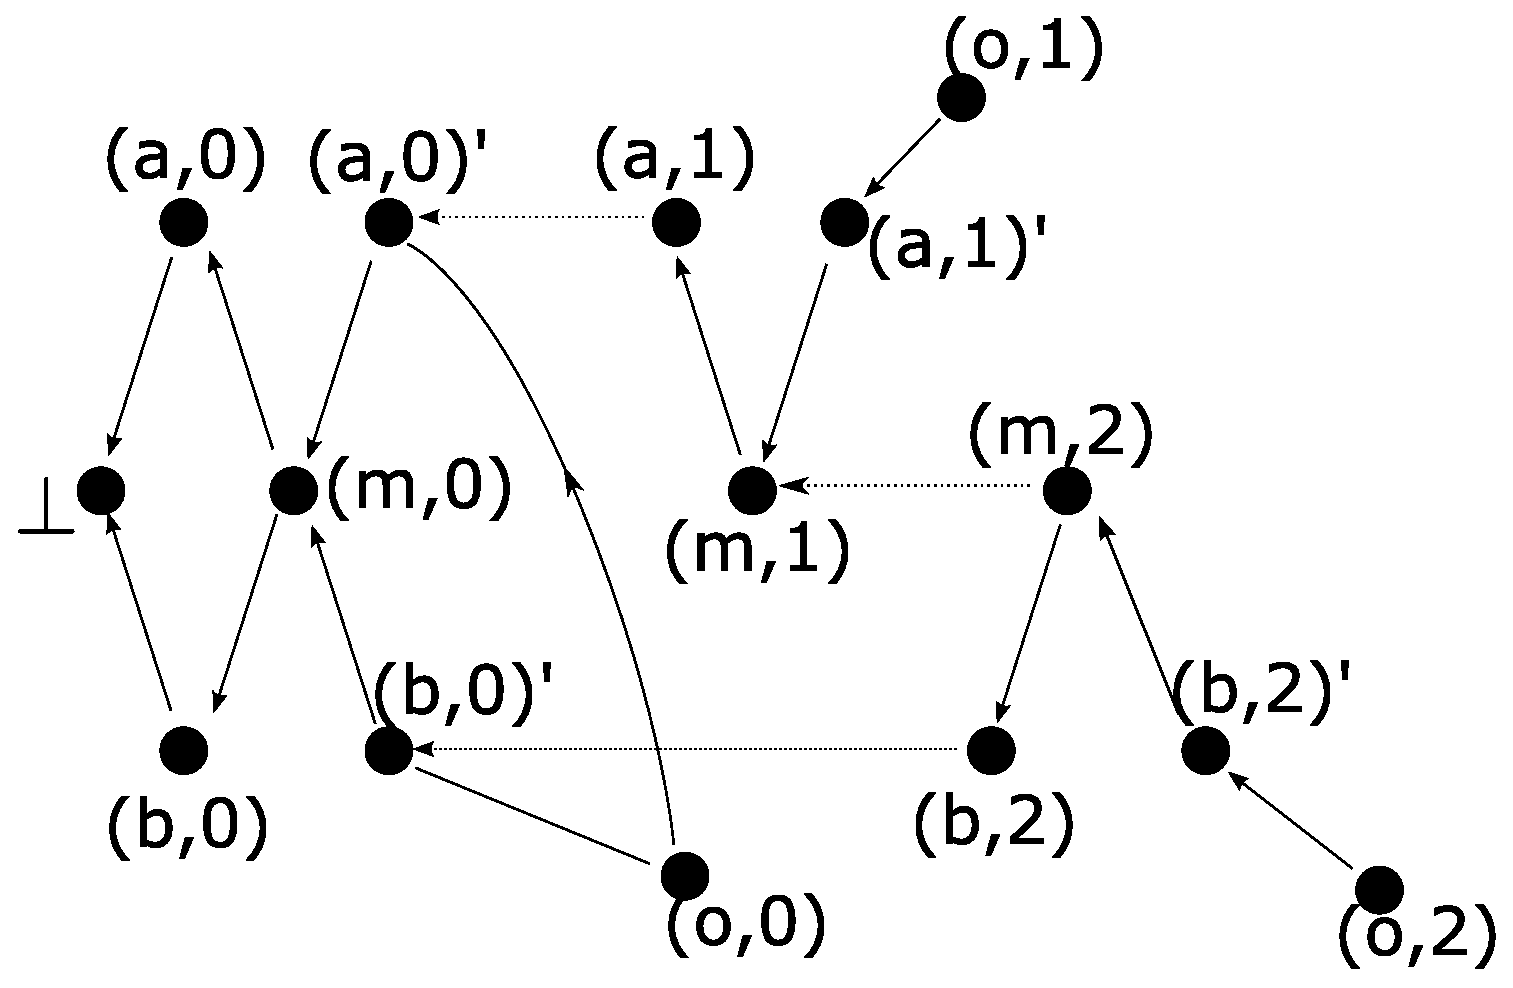
\includegraphics[scale=0.3]{schedulemodel.eps} 
\end{center}
\caption{A model $R(\cdot, \sigma)$
 induced by the partial schedule $\sigma = \left(\{a,b\}, \{a\}, \{b\}\right)$.
 A solid arrow pointing to $(x,n)$ shows an $f_x$ mapping.  Dotted arrows show $\preceq$ relations.
 We omit implied arrows and the valuation.}
 \label{schedulemodel}
\end{figure}

We can state the logical characterisation of waitfree communication.
\begin{theorem}[Completeness for waitfree communication]
\label{sc-comp}
 Assume $\varphi\supset \psi$ is a waitfree assertion.
 The relation $\vdash_{SC} \varphi\supset\psi$ holds if the relation $R(\varphi, \sigma),
 (o,n) \models \psi$ holds for any compatible partial schedule $\sigma$ where the state~$(o,n)$
 is the last state of the waitfree model $R(\varphi, \sigma)$.
\end{theorem}
To prove completeness, we only use special models called singleton
models induced by a permutation of processes.

\begin{definition}
 For a set of processes $P$, we define $\mathsf S(P)$ to be the set of the permutations of $P$.
\end{definition}

\begin{definition}
 For $\pi\in \mathsf S(P)$ and $0\le k\le |P|$, we define
 $SC(\pi,k)$ to be the set $\{K_\memory K_a I_a\supset K_\memory K_b I_b\mid b\le a\mbox{ in }\pi_0,\ldots \pi_k\}$.
\end{definition}

\begin{lemma}
 \label{perm}
 $\vdashsc \bigvee_{\pi\in \mathsf S(A)} SC(\pi, |P|)$ holds.
\end{lemma}
\begin{proof}
 It suffices to use rule (SC) many times.
\end{proof}

\begin{definition}
 For a permutation $\pi$ of $P$ and a waitfree protocol description $\varphi$, we
 define a partial schedule $\sigma(\varphi, \pi)$ as
\[
 \sigma(\varphi, \pi) = 
 \overbrace{\pi_0, \cdots, \pi_0}^{count_{\pi_0}(\varphi)},
 \overbrace{\pi_1, \cdots, \pi_1}^{count_{\pi_1}(\varphi)},
 \cdots \cdots
 \cdots,
 \overbrace{\pi_n,\cdots, \pi_n}^{count_{\pi_n}(\varphi)}.
\]
\end{definition}

\begin{definition}
 A singleton model is a model of the form $R(\varphi, \sigma(\varphi,
 \pi))$. We abbreviate this to $R(\varphi, \pi)$.

 For a singleton model and an index $k\in I$, $w_k$ denotes the minimum external
 observer state above all $\pi_j$~states for $j< k$.
\end{definition}

\begin{definition}
 For a waitfree protocol description $\varphi = \bigwedge_{a\in A} 
 \overbrace{K_a K_\memory K_a \cdots K_a}^{n_a}
 I_a$, we define the restriction \\
 $\varphi\restriction_{p,k} = 
 \bigwedge_{a\in A\restriction_{p,k}} \overbrace{K_a K_\memory K_a \cdots K_a}^{n_a} I_a$,
 where $A\restriction_{p,k} = \{a\mid p_j = a \mbox{ for some
 } j<
 k\}$.
\end{definition}

\begin{lemma}
 \label{stronger}
 $R(\varphi, \pi), (o,k)\models \psi\Longrightarrow SC(\pi, k)\vdash
 \varphi\restriction_{\pi,k}\supset\psi$.
\end{lemma}
\begin{proof}[Proof of Lemma~\ref{stronger}]
 By induction on $k$.
\begin{description}
 \item[(Case $k=0$)] 
 We show a stronger proposition:
$
 (o,0)\models \psi \quad\Longrightarrow\quad f_{p_0}(o,0)\models \psi,
 \vdash \varphi\restriction_{p,0}\supset \psi
 \mbox{ and }
 \vdash \varphi\restriction_{p,0}\supset K_a\psi.
$
by inner induction on $\psi$.
\begin{description}
 \item[(When $\psi$ is an atomic formula $P$)] 
 $P = I_{\pi_0}$ holds.
 Since $\varphi\restriction_{\pi,0} = K_{\pi_0}K_\memory K_{\pi_0}\cdots K_\memory K_{\pi_0}I_{\pi_0}$,
 $\vdash\varphi\restriction_{\pi,0}\supset K_{\pi_0}P$ holds.
 So, $SC(\pi,0)\vdash \varphi\restriction_{\pi,0}\supset K_{\pi_0}P$ holds.
 Consequently, $SC(\pi,0)\vdash \varphi\restriction_{\pi,0}\supset P$ also holds.
 \item[(When $\psi = \psi_0\wedge \psi_1$ or $\psi_0\vee\psi_1$)] 
 Induction goes smoothly.
 \item[(When $\psi = K_a\psi'$)]
 Assume $(o,0)\models K_a\psi'$. Claim: $a=\pi_0$ holds.
 Seeking contradiction, assume $a\neq \pi_0$.
 That means $f_a(o,0) = \bot$.
 However, waitfree task specification is satisfied at the state $\bot$.
 Contradiction.
 We have proved $a=\pi_0$. Using this, we can show that $f_a(o,0)\models\psi'$ holds.
 By idempotency of $f_a$, $f_a(f_a((o,0)))\models \psi'$ holds.
 This means $f_a((o,0))\models K_a\psi'$.
 Since $(o,0)\models \psi'$, by inner induction hypothesis,
 $\vdash \varphi\restriction_{\pi,0}\supset K_a\psi_a'$.
 By proof theoretic consideration,
 $\vdash \varphi\restriction_{\pi,0}\supset K_a K_a\psi'$ holds.
\end{description}
 \item[(Case $k = k' + 1$)]
 Like the base case, we show a stronger proposition
$
 (o,k)\models \psi\Leftrightarrow f_{\pi_k}((o,k))\models \psi \Rightarrow SC(\pi,k)\vdash
 \varphi\restriction_{\pi,k}\supset \psi\mbox{ and }SC(\pi,k)\vdash
 \varphi\restriction_{\pi,k}\supset K_{\pi_k}\psi, 
$
using induction on $\psi$.
\begin{description}
 \item[(When $\psi = P$, an atomic formula)] 
 Either $R(\varphi, \pi), w_{k'}\models P$ or $I_{\pi_k}=P$ holds.
 In the former case, by induction hypothesis.
 In the latter case, similarly as the base case.
 \item[(When $\psi = \psi_0\wedge \psi_1$ or $\psi_0\vee\psi_1$)] 
 Induction goes smoothly.
 \item[(When $\psi = K_x\psi'$)] 
If $\pi_k\neq x$, $f_{\pi_k}((o,k))\models K_x\psi'$ implies $(o,k')\models K_x\psi'$.
	    By outer induction hypothesis, $SC(\pi,k')\vdash
	    \varphi\restriction_{\pi,k'}\supset K_x\psi'$ and
	    $SC(\pi,k')\vdash \varphi\restriction_{\pi,k'}\vdash
	    \varphi\restriction_{\pi,k'}\supset K_x\psi'$ hold.
	    Here, we can safely replace $k'$ with $k$.
	    If $\pi_k=x$, $(o,k)\models K_x\psi'$ imply
	    $(o,k)\models \psi'$.
	    By inner induction hypothesis, we obtain
	    $SC(\pi,k)\vdash\varphi\restriction_{\pi,k}\supset K_x\psi'$.
	    This also implies $SC(\pi,k)\vdash\varphi\restriction_{\pi,k}\supset K_xK_x\psi'$.
\end{description}
\end{description}
\end{proof}
After showing this generalised lemma, proving Theorem~\ref{sc-comp} is
easy.
\begin{proof}[Proof of Theorem~\ref{sc-comp}]
 Since $R(\varphi, p), w_{|P|}\models \psi$, $SC(p,|P|)\vdash \varphi\supset
 \psi$.
By Lemma~\ref{perm}, $\vdashsc
 \varphi\supset \psi$.
\end{proof}
Any models induced by a partial schedule is finite.  For a waitfree assertion $\varphi$,
it is decidable whether $\vdashsc \varphi$ holds or not.


\subsection{Decidability of Solvability of Waitfree Task Specification}

\begin{definition}
 A waitfree task specification $\psi$ is solvable if there is such a
 waitfree protocol description $\varphi$ that the relation
 $R(\varphi,\sigma), (o,n)\models\psi$ holds for any compatible partial
 schedule $\sigma$ where the state $(o,n)$ is the last state of the
 model $R(\varphi,\sigma)$.
\end{definition}

\noindent \textbf{Fact.} The set of solvable waitfree task specifications are
recursively enumerable because the relation $\vdashsc$ is axiomatised.

\noindent \textbf{Fact.} The set of unsolvable waitfree task
specifications are recursively enumerable because partial schedule-induced
models are recursively enumerable.

\begin{theorem}
 \label{wf-dec}
 It is decidable whether a waitfree task
specification is solvable or not.
\end{theorem}
\begin{proof}
These two facts imply that it is decidable whether a waitfree task
specification is solvable or not.
\end{proof}

This does not contradict to the undecidability
 of waitfreely solvable tasks by Gafni and
 Koutsoupias~\cite{gafni1999three}
 because the undecidability proof
utilises tasks that cannot be expressed by waitfree task specifications.
They use tasks involving consensus:
the tasks involving making agreements among processes, where
whether an output value is allowed or not depends on other processes'
output values.  Waitfree task specifications cannot describe such tasks.

\section{Related Work}
\label{related}

Van Benthem~\cite{van2009information} investigates the connection between
intuitionistic logic and information dynamics.  He speculates:
\begin{quotation}
It might be
that intuitionistic logic points the way towards a grand synthesis of information analysis
in the standard model-theoretic style with the dynamic view of logic as embodied
in proof and games.
\end{quotation}
This paper replies his speculation by defining knowledge in terms of BHK-interpretation
and defining a proof system \iec\,embodying the interpretation.

Ondrej Majer's 
Epistemic Logic with Relevant Agents~\cite{majer-epistemic}
is similar to \iec\, in that both logics have epistemic modalities and that both logics are
not classical.
However, the logic given in~\cite{majer-epistemic}
 contains only one modality $K$ for knowledge.
This implicitly assumes that there is a single agent, not multiple agents so that it is
impossible for their logic to treat communication between multiple agents.

Many logics have both temporal and epistemic modalities~\cite{sato13study, wozna2005logic}.
Ewald~\cite{1986} proposes an intuitionistic logic with temporal modality.
We unify the intuitionistic semantics and temporal semantics so that the logic
\iec\,lacks temporal modality yet represents some temporal notions.
Adding a temporal modality like Ewald~\cite{1986} would increase the expressivity of the
logic, but it would complicate the syntax and semantics.
We would like to investigate the simple logic \iec\,first
 and then expand \iec\,with
additional constructs.

In Kobayashi and Yonezawa's logic~\cite{kobayashi1995asynchronous}, processes
appear in formulas but time does not appear in formulas
because time is implicit in the system of logic programming.
This logic is different from \iec\, in that this logic is based on linear logic and that their
usage is logic programming.

Belnap and Harper's ``seeing to it that'' (stit) logical operator
aims at describing interaction between agents.
The semantics for the operator involves both agency and temporal notion, which is more
complicated than the meaning of $K_a$ operator in \iec.
A fundamental difference of the stit operator and the epistemic operator in \iec\,
is whether the modalities mention the future or tha past.
The stit operator mentions the future while the epistemic operator mentions the past.

Dynamic epistemic logic is a logic that aims at reasoning about communication.
However the semantics of the logic involves
instantaneous change of models.
We argue such instantaneous change of the whole world it is
not a natural description of asynchronous communication.


\section{Conclusion}
\label{conclusion}

We defined an intuitionistic modal logic called intuitionistic epistemic logic (\iec\,for
short).
We defined both a natural deduction system and a Kripke model for it.
We proved both soundness and strong completeness.
The deduction system of \iec\,is similar to that of classical epistemic logic,
but lacks negative introspection and double negation elimination and has distribution of
disjunction over epistemic modalities instead.
The semantics of \iec\,is similar to that of intuitionistic propositional logic,
but has an additional function on the states for each agent, which we call a modal function.
We defined the syntactic counterpart of the modal function and used it for extending Aczel's
slash and proving disjunction property of \iec.  The syntactic counterpart of the modal
function was also useful for proving strong completeness and finite model property for
\iec.
By disjunction property, we know that the logic \iec\,is a constructive logic.
Also, decidability suggests the possibility of typed lambda calculus using \iec\,as the
typing system.

On the logic~\iec, we analysed the concept of sequential consistency and wait-free
communication.
The deepness of our anlaysis is represented in a deep proof tree (Figure~\ref{hoge}) for a
property of a relatively simple and small wait-free protol involving two processes.
Distributed programming over shared memory can be seen as a game involving the scheduler
and the program.
Logic can be seen as a game involving the models and the formulas.
We modelled schedules as a model of logic and programs as formulas.
Since sequential consistency is a restriction on schedules,
we modeled sequential consistency as a restriction on models.
The restriction on the models representing sequential consistency could actually
axiomatized using an axiom type that is similar to the axiom type for prelinerity defining
a famous intermediate logic.
Since waitfreedom is a restriction on programs,
we modelled waitfree programs as a set of formulas called waitfree protocol description.
We also modelled specification for waitfree programs as a set of formulas called waitfree
task specification.
We used a waitfree assertion, which is
an implication formula consisting of a waitfree protocol description and a
waitfree task specification,
 to represent 
an assertion that a waitfree protocol meets a specification.


\section{Discussion}
\label{discuss}

\subsection{Waitfree Computation}
\label{Shavit}
The G\"{o}del Prize in 2004 was given to Herlihy and Shavit~\cite{herlihy1999topological}
and
Saks and Zaharoglou~\cite{saks2000wait}.
This work was motivated by these works.
Herlihy and Shavit~\cite{herlihy1999topological} used
 subdivision of coloured simplicial complex to model
waitfree computation. Each vertex is coloured by an agent. Each simplex contains vertices
with distinct colours. A vertex may have an ancestor simplex called carrier.
The minimum subset of $(S\cup V) \times (S\cup V)$
 containing the ancestor relation and the relation $\in$ forms an order $\sqsubset$.
We can define a partial
 $f_a: S\rightarrow S$ where $S$ is the set of simplex in
a simplicial complex by letting $f_a(s) = \{x\}$ where $x$ is the maximum vertex below $s$
(w.r.t. $\sqsubset$)
 whose colour is
$a$. When we add a bottom simplex $\bot$ and make $f_a$ total, we can regard
a~simplicial complex as a~model of \iec\, as in an example (Figure~\ref{subdivision}).
\begin{figure}
 \begin{center}
  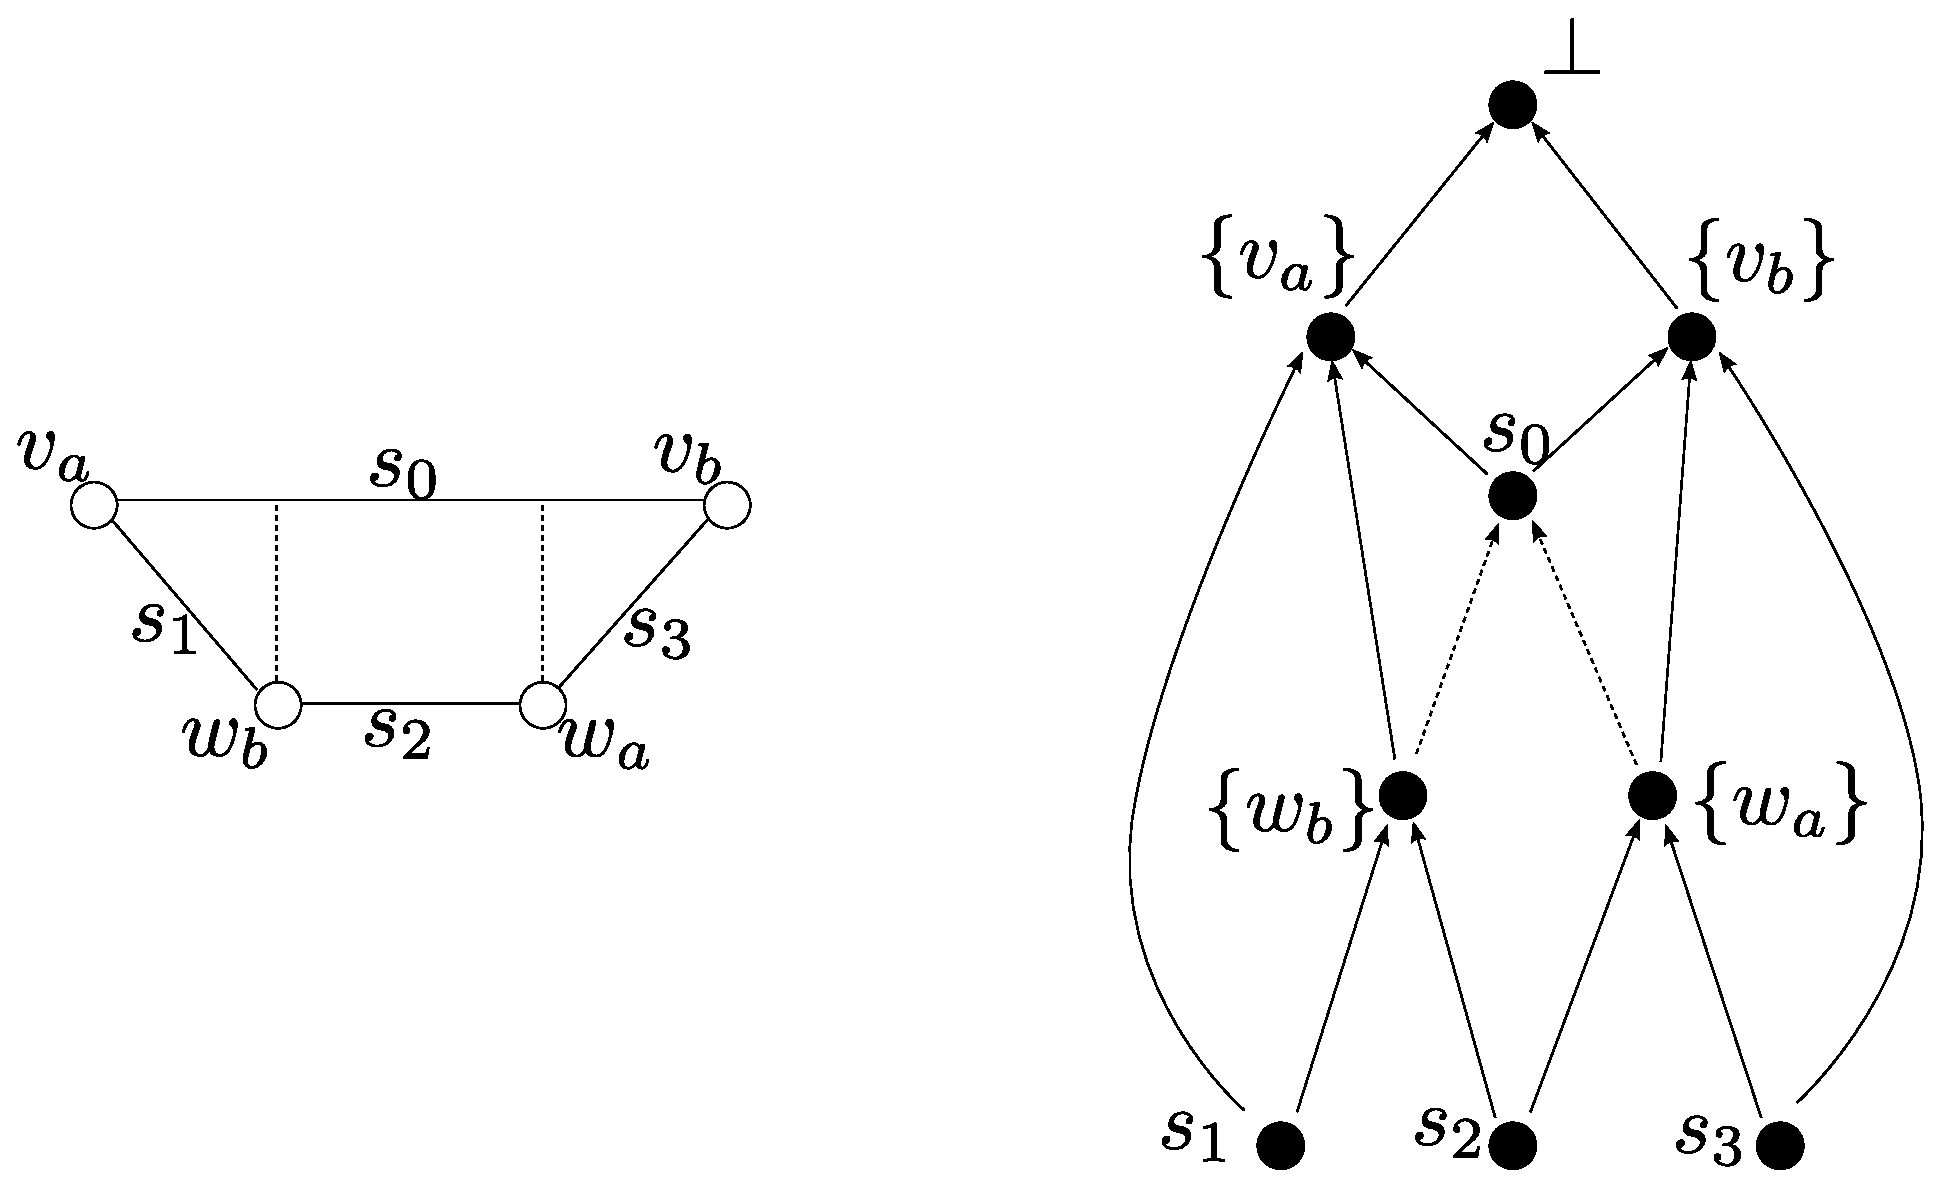
\includegraphics[scale=0.3]{subdivision_original.eps}
 \end{center}
 \caption{How subdivision of simplicial complexes is transformed into \iec\, model.
Left: A simplex $s_0 = \{v_a, v_b\}$ is subdivided into $s_1 = \{v_a, w_b\}, s_2
 = \{w_a, w_b\}$ and $s_3 = \{w_a, v_b\}$. Right: \iec\, frame obtained from the left
 subdivision.}
\label{subdivision}
\end{figure}

Saks and Zaharoglou~\cite{saks2000wait} use full-information protocol~\cite{182113}.
Even the shared variables remember the whole history.
In every component, knowledge increases monotonically through time.
This monotonicity suggests that their model can be analysed effectively in Kripke models
for intuitionistic logic.
Saks and Zaharoglou~\cite{saks2000wait} also suggest that 
``We believe that it will be worthwhile to explore the
connection with the formal theory of distributed
knowledge.'' This work is following their remark in treating waitfree communication in a
formal way, especially using a logic with epistemic modality.

\subsection{Sequential Consistency or Linearizability}

Attiya and Welch~\cite{attiya1994sequential} pointed out that 
sequential consistency~\cite{lamport1979make} and
linearizability~\cite{herlihy1990linearizability} are often confused.
We briefly make sure that the deduction system $\vdash_{SC}$ does
not characterise linearizability.
Herlihy~\cite{herlihy1990linearizability} stated that
linearizability is a local
property; in other words,
when each memory object satisfies linearizability, the combined system also has linearizability.
However, the axiom type $SC$ is not local.
To see that, assume there are two memory objects $\memory$ and $\memory'$.
The axiom type $SC$ for $\memory$ is $(K_\memory \varphi\supset K_\memory
\psi)\vee (K_\memory \psi\supset K_\memory\varphi)$.
The axiom type $SC$ for $\memory'$ is $(K_{\memory'} \varphi\supset K_{\memory'}
\psi)\vee (K_{\memory'} \psi\supset K_{\memory'}\varphi)$.
Even when both of these axiom types are available,
the~\textit{mixed} axiom type $(K_{\memory'} \varphi\supset K_{\memory}
\psi)\vee (K_{\memory} \psi\supset K_{\memory'}\varphi)$ is not derivable. This shows
the characterised property is not local.

\subsection{Other Consistency Models}

Steinke and Nutt~\cite{steinke2004unified} gave a lattice of consistency properties
including: sequential consistency, causal consistency, processor consistency, PRAM
consistency, cache consistency, slow consistency and local consistency.
It is our future work modelling other consistency properties.

\subsection{The Cost of Monotonic Reasoning: Latency versus Throughput}

The logic \iec\,is more suitable in a situation where latency is more important than throughput.
Since we consider time as the partial order of intuitionistic Kripke models,
all knowledge must be preserved during time progress.
Communication must be done in full-information manner (as in
full-information protocols in~\cite{182113}) because messages
define the partial order.
 Although there are some methods~\cite{182113, halpern1990knowledge, halpern1987using,
 halpern1985formal}
  for extracting implementable protocols from
 full-information protocols, 
Our logic is advantageous when latency is important so that
it is important to know how many message interactions are needed to accomplish a certain
task.  We plan to investigate network protocols with \iec.

We speculate that replacing intuitionistic modalities with
linear modalities might enable us to deal with throughput oriented properties.

\subsection{$\lambda$-calculus} 

It would be interesting to consider reduction of proofs
because it leads to typed programming language for asynchronous communication.

\subsection{Disjunction Distribution Over $K$~Modality}

Since the semantics for modalities is defined by functions on Kripke frames,
the disjunction distributes modalities in \iec.
Kojima and Igarashi~\cite{kojima2008constructive} avoids the distribution of modalities 
over disjunction by giving up functional modality.
On the other hand, \iec\,has distribution of modalities over disjunction.
We speculate that the difference comes from the interpretation of modalities according to
time:
in \cite{kojima2008constructive}, 
inner subformulas within the scope of the modality are interpreted in the future; while
in \iec, inner subformulas within the scope of the modalities are interpreted in the past.

By translation of Suzuki~\cite{suzuki1990kripke},
when $A$ is a singleton set, a model of \iec\,corresponds to 
a model of intuitionistic predicate logic with singleton domain
in the same manner a model of the logic 
$\mathrm L_3$ of Ono~\cite{hiroakira-some} corresponds to the models of
intuitionistic predicate logic with constant domain.
This fact suggests that the semantics of \iec\, is very simple when $A$ is a singleton set.
Simplicity was our aim at the beginning.

\subsection{Relationship with Intuitionistic Predicate Logic}

The translation of Suzuki~\cite{suzuki1990kripke} suggests
\iec\,with
a single agent corresponds to a singleton domain.
In intuitionistic predicate logic, the quantifiers $\forall$ and $\exists$ quantify over
elements of domain.
These facts suggest
quantification over the set of agents like $\forall x K_x\varphi$.
From the logic allowing such quantification,
we speculate that, by the method of program extraction,
we can obtain programs whose input and output contain names of agents.

Also, extending the translation of Suzuki|~\cite{suzuki1990kripke} to intuitionistic logic
with multiple modailities would be an interesting work.


\chapter{Finite Model Property for Sequential Consistency Logic}

\fix{just put NASSLLI paper here.}

\chapter{Waitfree Protocols in Logical Form}


\section{Introduction}

We proved finite model property of a class of intermediate modal logics
using analytic tableaux.
The target logics have Kripke frames where modalities are interpreted as
functions over the frame.  Moreover, each logic is parametrized by a
set of restrictions.  Each restriction is a disjunction of some
inequalities posing restrictions on the shape of the frame.

The target class of intermediate modal logics is a generalization of
intuitionistic epistemic logic proposed by Hirai~\cite{hirailpar}.
He used intuitionistic epistemic logic in order to model shared memory
consistencies, which are criteria that guarantees levels of
synchronization among different processes.
Both shared memory consistencies and some intermediate modal logics
can be characterized as a restriction on
partially-ordered structure:
Kripke frames for intermediate modal logics
and executions for shared memory
consistencies~\cite{steinke2004unified}.
He regarded Kripke frames as executions in order to translate
an intermediate modal logic into a shared memory
consistency.

However, he did not show finite model property for those
intermediate modal logics.  When software engineers talk about shared
memory consistencies, they assume an execution is finite.
When we think of Kripke models as executions, we are obliged to show
that the model is finite.
Especially when we want to construct a specific counterexample execution,
we have to build a \textit{finite} Kripke model.

For example,
under \textit{sequential consistency logic}, which is intuitionistic epistemic
logic along with the axioms of the form
$(K_m\varphi\supset K_m\psi) \vee (K_m\psi\supset K_m\varphi)$,
the formula $K_aK_mK_aI \supset K_bK_mK_bJ\supset K_bI$ is not a
theorem.
In terms of shared memory consistency, this means that even when a
process~$a$ has put information~$I$ on the shared memory and got a
successful acknowledgement from the shared memory and the other
process~$b$ does the same with information~$J$, it is not always the
case that process~$b$ has obtained information~$I$\kern -2pt.
In other words, there are executions without this property.
This can be confirmed via
finite model property for sequential consistency logic.
We show this property in a generalized form.

\section{The Target Logics}
 \label{logic}

The class of logics that we consider is a generalization of
intuitionistic propositional logic.
The class of logics also contains G\"{o}del--Dummett logic~\cite{dummett59}
and the intuitionistic epistemic logic proposed by 
Hirai~\cite{hirailpar}.
Let us assume that
there are a countably infinite set~$\pvar$ of \textit{propositional variables} and a 
finite set~$\agents$ of \textit{agents}. 

\begin{definition}
We define the set~$\fml$ of formulas by BNF:
\[
 \varphi,\psi ::= \bot\mid I\mid K_a\varphi\mid (\varphi\vee\psi)\mid
 (\varphi\wedge\psi)\mid (\varphi\supset\psi)
\]
 where $a$ is an agent in $\agents$
 and $I$ is a propositional variable in~$\pvar$.
\end{definition}

For a set of formulas $\Gamma\!$, notation $K_a\Gamma$ denotes the set
$\{K_a\varphi\mid\varphi\in\Gamma\}$\enspace.

\begin{definition}[Kripke frame]
A \textit{frame} $\tuple{W,\preceq,(f_a)_{a\in \agents}}$ is a tuple where
\begin{itemize}
 \item $\tuple{W,\preceq}$ is a partially ordered set, and
 \item each $f_a\colon W\rightarrow W$ is a monotonic function with
       respect to~$\preceq$.
\end{itemize} 
\end{definition}

\begin{definition}[Kripke model]
A \textit{model} $\tuple{W,\preceq, (f_a)_{a\in \agents},\rho}$ is a tuple where
\begin{itemize}
 \item $\tuple{W,\preceq,(f_a)_{a\in \agents}}$ is a frame, and
 \item $\rho\colon \pvar\rightarrow 2^W$ is a function that maps every
       propositional variable to a upward-closed subset of $W\!$.
\end{itemize} 
\end{definition}

We are going to prove finite model property for a class of
intermediate modal logics.  The logics are parametrized with
world restriction sets,  which we are going to define.
We assume that there is a countably infinite set of \textit{world
variables}~$\wvar$.
We use $\mathsf v, \mathsf w,\ldots$ to denote world variables.
We define \textit{world terms} using BNF:
\[
 \mathsf s::=\mathsf v\mid \mathsf s.a
\]
where $a$ is an agent.
Every world term can be written as $\mathsf v.s$ where $s$ is a fintie sequence
of agents (a postfix).
A \textit{world inequality} is an inequation of the form $\mathsf s\le
\mathsf t$ where $\mathsf s$ and $\mathsf t$ are world terms.
\begin{definition}
A world restriction is a sequence of world inequalities jointed
 by~$\wor$ formed like
 $\mathsf v_0.s_0\le\mathsf v_1.t_1\wor\cdots\wor
 \mathsf v_{n-1}.s_{n-1}\le\mathsf v_n.t_n\wor \mathsf v_n.s_n\le\mathsf
 v_0.t_0$ that satisfies either
 \begin{itemize}
  \item (single clause) $n=0$, or
  \item (single postfix) $s_i = t_i = s_j = t_{j}$ for $0\le i,j\le n$.
 \end{itemize}
\end{definition}
A \textit{world restriction set} is a finite set of world restrictions.

A \textit{world valuation} maps a world variable into a world of a frame.
We extend a world valuation on world variables
$\delta\colon\mathcal V_W\rightarrow W$ to that on world terms
inductively as $\delta(\mathsf s.a)=f_a(\delta(\mathsf s))$.
A frame $\tuple{W,\preceq, 1,(f_a)_{a\in\agents}}$ satisfies a world inequality
$\mathsf s\le\mathsf t$ iff $\delta(\mathsf s)\preceq \delta(\mathsf t)$
for all $\delta\colon\mathcal V_W\rightarrow W$.
A frame~$F$ satisfies a world restriction $\mathsf r$
iff $M$ satisfies $\delta(\mathsf r)$ for any world valuation~$\delta$.
For example, a frame satisfies $\mathsf v\le \mathsf w\wor\mathsf
w\le\mathsf v$ iff the frame is totally ordered.
An $\mathsf R$-frame is a frame that
satisfies all world restrictions in~$\mathsf R$.
An $\mathsf R$-model is a model with an $\mathsf R$-frame.


\begin{definition}
 We define the \textit{validity relation} $M,w\models\varphi$ over a model
 $M = \tuple{W,\preceq,(f_a)_{a\in \agents},\rho}$, a state~$w\in W$ and a
 formula~$\varphi$ inductively on $\varphi$.
 In this definition, let
 us abbreviate $M,w\models \varphi$ into $w\models \varphi$\enspace.
\newcommand{\m}{}
\begin{itemize}
\item $w\models \bot$ never holds.
\item $w\models I$ iff
$w \in
 \rho(I)$.
\item	    $w\models K_a \psi$ iff
	    $f_a(w)\models \psi$.
\item $w\models \psi_0\wedge\psi_1$ iff both
 $w\models \psi_0$ and $w\models \psi_1$ hold.
\item
 $ w\models \psi_0\vee\psi_1$ iff either
 $ w\models \psi_0$ or $w\models \psi_1$ holds.
\item
	   $w\models \psi_0\supset\psi_1$ iff 
	   $w'\succeq w$ and $w'\models \psi_0$ imply
	   $w'\models\psi_1$ for any $w'\in W$\enspace.
\end{itemize}
\end{definition}
A model~$M$ \textit{satisfies} $\varphi$ iff $M,w\models\varphi$ holds for any
state~$w$ of~$M$.
A formula~$\varphi$ is \textit{valid under} $\mathsf R$ iff
every $\mathsf R$-model~$M$ satisfies $M\models \varphi$.
For this, we write $\modelsR \varphi$\enspace.

\begin{lemma}[Kripke monotonicity]
 \label{monot}
 $M,w\models\varphi$ and $w\preceq v$ imply 
$M,v\models\varphi$.
\end{lemma}
\begin{proof}
 Induction on~$\varphi$.
 We use monotonicity of $f_a$ here.
\end{proof}

\paragraph{The proof system.}
Since both $\pvar$ and $\wvar$ are countably infinite,
there is an injection that maps a world variable to a propositional
variable.
We fix one such injection
$\mathsf w\mapsto I_{\mathsf w}$.
Inductively on the construction of world terms,
we assign a formula~$[\mathsf t]$ to every world term~$\mathsf t$:
\begin{itemize}
 \item for a world term $\mathsf w\in \wvar$, we define $[\mathsf w]$ to be
       $I_{\mathsf w}$,
 \item for a world term $\mathsf{s.a}$, we construct
 a formula $[\mathsf{s.a}]$ by
replacing every propositional variable~$P$ with $K_aP$ in $[\mathsf s]$.
\end{itemize}
Note that the sequence $\mathsf{.a.b.c}$ is translated into the same
order $K_a K_b K_c$ although a postfix is translated into a prefix.
We define $K_s\varphi$ as $[\mathsf w.s][\varphi/I_{\mathsf w}]$.
Also, we define $f_b\circ f_a$ as $f_{ab}$.  This ensures $M, w\models
K_s\varphi\Leftrightarrow M,f_s(w)\models\varphi$.

This translation of world terms into formulas
enables us to translate world inequalities and world restrictions
into formulas:
\begin{itemize}
 \item $[\mathsf s\le \mathsf t] := [\mathsf s]\supset [\mathsf t]$, and
 \item $[\mathsf{s_0}\le \mathsf{t_0}\wor \cdots\wor \mathsf{s_n}\le \mathsf{t_n}] := [\mathsf{s_0}\le \mathsf{t_0}]\vee
       \cdots \vee [\mathsf{s_n}\le \mathsf{t_n}]$ \enspace.
\end{itemize}

We define $\mathbf{Ax}(\mathsf R)$ to be the substitution closure of
$\{[\mathsf r]\mid \mathsf r\in \mathsf R\}$.
The substitution closure of a set~$S$ of formulas is defined as
$\{\varphi[\psi/P]\}$ where $\psi$ run freely on~$\fml$ and $P$ on~$\pvar$.

\begin{figure}[t]
\begin{center}
 \def\fCenter{\vdashR}
\AxiomC{}
\LeftLabel{(axiom)}
\UnaryInf$\varphi \fCenter \varphi$
 \DisplayProof
\hfill
\Axiom$\Gamma\fCenter\varphi$
\LeftLabel{(weakening)}
 \UnaryInf$\psi,\,\Gamma\fCenter\varphi$
\DisplayProof
 \hfill
\Axiom$ \varphi,\,\varphi,\,\Gamma\fCenter\psi$
\LeftLabel{(contraction)}
\UnaryInf$\varphi,\,\Gamma\fCenter\psi$
\DisplayProof
\ruleskip
\Axiom$\Gamma, \varphi,\psi,\, \Gamma'\fCenter\theta$
\LeftLabel{(exchange)}
\UnaryInf$\Gamma,\,\psi,\varphi,\,\Gamma'\fCenter\theta$
\DisplayProof
\hfill
\Axiom$\Gamma\fCenter\varphi$
\Axiom$\Gamma'\fCenter\psi$
\LeftLabel{($\wedge$-I)}
\BinaryInf$\Gamma,\Gamma'\fCenter \varphi\wedge\psi$
\DisplayProof
\hfill
\Axiom$\Gamma\fCenter \varphi$
\LeftLabel{($\vee$-I$_0$)}
\UnaryInf$\Gamma\fCenter \varphi\vee\psi$
\DisplayProof
\ruleskip
\Axiom$\Gamma\fCenter \varphi$
\LeftLabel{($\vee$-I$_1$)}
\UnaryInf$\Gamma\fCenter \psi\vee\varphi$
\DisplayProof
\hfill
\Axiom$\Gamma \fCenter\varphi\wedge\psi$
\LeftLabel{($\wedge$-E$_0$)}
\UnaryInf$\Gamma\fCenter \varphi$
\DisplayProof
\hfill
\Axiom$\Gamma\fCenter \varphi\wedge\psi$
\LeftLabel{($\wedge$-E$_1$)}
\UnaryInf$\Gamma\fCenter \psi$
\DisplayProof
\ruleskip
\Axiom$\Gamma\fCenter \psi_0\vee\psi_1$
\Axiom$\Gamma,\,\psi_0\fCenter \varphi$
\Axiom$\Gamma,\,\psi_1\fCenter \varphi$
\LeftLabel{($\vee$-E)}
\TrinaryInf$\Gamma\fCenter \varphi$
\DisplayProof
\vskip 5mm
\Axiom$\varphi,\,\Gamma\fCenter\psi$
\LeftLabel{($\supset$-I)}
\UnaryInf$\Gamma\fCenter \varphi\supset\psi$
\DisplayProof
\hfill
\Axiom$\Gamma\fCenter\psi_0\supset\psi_1$
\Axiom$\Gamma\fCenter \psi_0$
\LeftLabel{($\supset$-E)}
\BinaryInf$\Gamma\fCenter \psi_1$
\DisplayProof
\hfill
\Axiom$\Gamma\fCenter\bot$
 \LeftLabel{($\bot$-E)}
 \UnaryInf$\Gamma\fCenter\varphi$
 \DisplayProof
\ruleskip
\AxiomC{}
\LeftLabel{($\vee K$)}
 \UnaryInf$K_a(\varphi\vee\psi)\fCenter (K_a \varphi)\vee K_a\psi$
\DisplayProof
 \hfill
 \AxiomC{}
 \LeftLabel{($\varphi\in \mathbf{Ax}(\mathsf R)$)}
 \UnaryInf$\fCenter\varphi$
 \DisplayProof
 \ruleskip
 \Axiom$\Gamma\fCenter\varphi$
 \LeftLabel{(necessitation)}
 \UnaryInf$K_a\Gamma\fCenter K_a\varphi$
 \DisplayProof
\end{center}
\caption{Deduction rules of $\vdashR$.}
\label{fig}
\end{figure}

\begin{definition}
 We define the proof system $\vdashR$ by Fig.~\ref{fig}.
\end{definition}

\begin{theorem}
 \label{sound-comp-nat-kripke}
 $\Gamma\vdashR\varphi\Longleftrightarrow\Gamma\modelsR \varphi$\enspace.
\end{theorem}
We put the proof in Appendix~\ref{app} because the method is
standard.

\subsection{Examples}

\paragraph{Classical logic.}
When
$\mathsf R = \{\mathsf v\le\mathsf w\wor\mathsf w\le\mathsf x\wor\mathsf x\le\mathsf
v\}$,
the corresponding axioms can be obtained as follows:
\begin{align*}
[ \mathsf v\le \mathsf w\wor \mathsf w\le\mathsf x\wor \mathsf x\le\mathsf v ] &=
(I_{\mathsf v}\supset I_{\mathsf w})\vee (I_{\mathsf w}\supset
I_{\mathsf x})\vee (I_{\mathsf x}\supset I_{\mathsf v})
\\
\mathbf{Ax}(\mathsf R) = \mathbf{Ax}(\{\mathsf v\le\mathsf w\wor \mathsf
w\le \mathsf x \wor \mathsf x\le\mathsf v\}) &= \{(\varphi\supset\psi)\vee(\psi\supset\chi)\vee(\chi\supset\varphi)\}.
\end{align*}
$\mathbf{Ax}(\mathsf R)$ is equivalent to the excluded middle so $\mathsf R$ defines
classical logic.

\paragraph{G\"{o}del--Dummett logic.}
When $\mathsf R=\{\mathsf v\le\mathsf w\wor\mathsf w\le\mathsf v\}$,
the corresponding axioms can be obtained as follows:
\begin{align*}
[\mathsf v\le \mathsf w\wor \mathsf w\le\mathsf v] &=
(I_{\mathsf v}\supset I_{\mathsf w})\vee (I_{\mathsf w}\supset
I_{\mathsf v})\\
\mathbf{Ax}(\mathsf R) = \mathbf{Ax}(\{\mathsf v\le\mathsf w\wor \mathsf
w\le \mathsf v\}) &= \{(\varphi\supset\psi)\vee(\psi\supset\varphi)\mid
\varphi,\psi\colon\mbox{formula}\}.
\end{align*}
$\mathbf{Ax}(\mathsf R)$ coincides with the axioms of
G\"{o}del--Dummett logic~\cite{dummett59}.

\paragraph{Sequential consistency logic.}
When $\mathsf R=\{\mathsf v.\mathsf m\le\mathsf w.\mathsf m\wor \mathsf
w.\mathsf m\le \mathsf v.\mathsf m\}$,
the corresponding set of axioms
$\mathbf{Ax}(\mathsf R) = \{(K_{\mathsf m}\varphi\supset K_{\mathsf
m}\psi)\vee(K_{\mathsf m}\psi\supset K_{\mathsf m}\varphi)\mid \varphi,
\psi\colon\mbox{formula}\}$
 axiomatizes sequential consistency logic,
which is proposed by Hirai~\cite{hirailpar} for modeling a shared memory consistency called sequential consistency.


\section{Finite Model Property}
\label{fmp-proof}

This is our main result.
\begin{theorem}
 \label{fmp}
 $\vdashR\varphi$ holds iff $M\models \varphi$ holds
 for all finite {\sf R}-model $M$.
\end{theorem}

We use another deduction system\,\LB\,in order to obtain finite model
property.
The outline of the proof is these circular implications:
\begin{align*}
 \vdashRLB\varphi &\Longrightarrow \quad \models_{\mathsf R}\varphi\quad
 &(\mbox{by Lemma~\ref{sound}})\\
 &\Longrightarrow \quad \vdash_{\mathsf R}\varphi &(\mbox{by
 Thm.~\ref{sound-comp-nat-kripke}}) \\
 &\Longrightarrow\quad \modelsR\varphi &\mbox{(by Thm.~\ref{sound-comp-nat-kripke})}\\
 &\Longrightarrow\quad M\models\varphi \mbox{ for any finite $\mathsf
 R$-model }M\\
 &\Longrightarrow\quad \vdashRLB\varphi & (\mbox{by
 Lemma~\ref{R-fmp}})\enspace .
\end{align*}
This method extends Waaler
and Wallen's method for intuitionistic logic~\cite{waaler1999tableaux}.

\subsection{\LB}

The deduction system\,\LB\,uses \textit{prefixed formulas}.  A
prefixed formula is shaped like $\mathsf s::\varphi$ where $\mathsf s $
is a world term and $\varphi$ is a formula.
Informally, this prefixed formula means that the formula~$\varphi$ is
satisfied in a state referenced by~$\mathsf s$.
A \textit{sequent} is shaped like
  $\Theta\parallel \Gamma\longrightarrow \Delta$ where
$\Theta$ is a finite set of world inequalities and both
$\Gamma$ and $\Delta$ are finite sets of prefixed formulas.
In a sequent, world inequality
$\mathsf s\le \mathsf s$ must be in $\Theta$
 for any world term $\mathsf s$ occurring in $\Delta$ or $\Gamma$.

A set~$\Theta$ of world inequalities
\textit{conforms to} world restriction set~$\mathsf R$ when all of the
following hold:
\begin{itemize}
 \item $\mathsf s\le \mathsf t, \mathsf t\le \mathsf u\in
       \Theta\Longrightarrow
       \mathsf s\le \mathsf u\in\Theta$,
 \item If $\mathsf{s_0}\le \mathsf{t_0} \wor \mathsf{s_1}\le \mathsf
       {t_1}\wor
       \cdots\wor \mathsf{s_n}\le
       \mathsf{t_n}\in \bar{\mathsf R}$ and all of
       $\mathsf{s_0},\mathsf{s_1},\ldots,\mathsf{s_n},
       \mathsf{t_0},\mathsf{t_1},\ldots, \mathsf{t_n}$ appear in~$\Theta$, then,
       $\mathsf{s_i}\le \mathsf{t_i}\in\Theta$ for at least
       one~$\mathsf{i}$, where $\bar {\mathsf R}$ is the substitution
       closure of~$\mathsf R$,
 \item If $\mathsf s\le\mathsf t\in\Theta$ and both $\mathsf s.a$ and
       $\mathsf t.a$ appear in~$\Theta$, then $\mathsf s.a\le\mathsf
       t.a\in \Theta$.
\end{itemize}
We define $\mathsf R(\Theta)$ to be the set of the minimal
supersets of~$\Theta$ conforming to~$\mathsf R$.
For example, when $\mathsf R=\{\mathsf w\le \mathsf v\wor\mathsf v\le \mathsf
w\}$,
$\mathsf R(\{\mathsf w\le \mathsf w, \mathsf v\le \mathsf v\}) =
\{\{\mathsf w\le \mathsf v, \mathsf w\le \mathsf w, \mathsf v \le
\mathsf v\}, \{\mathsf v \le
\mathsf w, \mathsf w\le \mathsf w, \mathsf v\le \mathsf v\}\}$\enspace.
 When $\Theta$ is finite, so is $\mathsf R(\Theta)$ because $\mathsf
 R(\Theta)\subseteq \{\mathsf s\le\mathsf
 t\mid\mathsf s,\mathsf t\mbox{ appears in }\Theta\}$.

\begin{definition}
 The calculus\,\LB\,for a world restriction set~$\mathsf R$ is defined in Fig.~\ref{LB}.
 When $\mathsf w\le \mathsf w\parallel \rightarrow \mathsf
 w::\varphi$ is provable in \LB\,for~$\mathsf R$,
 we write $\vdashRLB\varphi$.
\end{definition}

\begin{figure}[t]
  \def\fCenter{\longrightarrow}
 \small
 \begin{center}
\ruleskip
  \Axiom$\Theta\parallel \Gamma\fCenter \mathsf s::\varphi,\Delta$
  \Axiom$\Theta\parallel \Gamma, \mathsf t::\psi \fCenter \Delta$
  \RightLabel{L$\supset$}
  \BinaryInf$\Theta, \mathsf s\le \mathsf t\parallel \Gamma, \mathsf t::\varphi\supset\psi
  \fCenter \Delta$
  \DisplayProof
  \ruleskip
  \Axiom$\Theta'\parallel \Gamma, \mathsf w::\varphi\fCenter
  \mathsf w::\psi,\Delta\quad\mbox{ for every }\Theta'\in \mathsf
  R(\Theta\cup\{\mathsf s\le \mathsf w\})$
  \RightLabel{R$\supset$}
  \UnaryInf$\Theta\parallel \Gamma \fCenter \mathsf s::\varphi\supset\psi, \Delta$
  \DisplayProof\\ ($\mathsf w$ does not appear in the conclusion)
  \ruleskip
  \Axiom$\Theta'\parallel \Gamma, \mathsf s.a::\varphi\fCenter\Delta$
  \RightLabel{L$a$}
  \UnaryInf$\Theta\parallel \Gamma, \mathsf s::K_a\varphi\fCenter\Delta$
  \DisplayProof
\hfill
  \Axiom$\Theta\parallel \Gamma\fCenter\Delta, \mathsf s.a::\varphi$
  \RightLabel{R$a$}
  \UnaryInf$\Theta\parallel\Gamma\fCenter\Delta, \mathsf s :: K_a\varphi$
  \DisplayProof
 \end{center}
 \caption{The inference rules of \LB. Modification of Fig.~3 of
 Waaler and Wallen~\cite{waaler1999tableaux}.
 Since $\mathsf R(\Theta\cup\{\mathsf s\le\mathsf w\})$ is finite,
 R$\supset$
 is finitely branching.}
\label{LB}
\end{figure}

\begin{figure}[ht]
 \def\fCenter{\longrightarrow}
 \Axiom$\Theta,\mathsf v\le\mathsf x\parallel\mathsf v::\varphi,\mathsf
 x::\psi\fCenter\mathsf v::\psi,\mathsf x::\varphi$
 \Axiom$\Theta,\mathsf x\le\mathsf v\parallel\mathsf v::\varphi,\mathsf
 x::\psi\fCenter\mathsf v::\psi,\mathsf x::\varphi$
 \RightLabel{R$\supset$}
 \BinaryInf$\mathsf w\le\mathsf w,\mathsf w\le\mathsf v,\mathsf
 v\le\mathsf v\parallel\mathsf v::\varphi\fCenter\mathsf v::\psi,\mathsf
 w::\psi\supset\varphi$
 \RightLabel{R$\supset$}
 \UnaryInf$\mathsf w\le\mathsf w\parallel\fCenter\mathsf
 w::\varphi\supset\psi,\mathsf w::\psi\supset\varphi$
 \RightLabel{R$\vee$}
 \UnaryInf$\mathsf w\le\mathsf w\parallel\fCenter\mathsf
 w::(\varphi\supset\psi)\vee(\psi\supset\varphi)$
 \DisplayProof
 
 \caption{A derivation for
 $\vdashRLB(\varphi\supset\psi)\vee(\psi\supset\varphi)$ where
 $\mathsf R=\{\mathsf v\le\mathsf w,\mathsf w\le\mathsf v\}$.
 In the figure, $\Theta$ stands for $\{\mathsf w\le\mathsf w,\mathsf
 w\le \mathsf v, \mathsf v\le\mathsf v, \mathsf w\le \mathsf x, \mathsf
 x \le \mathsf x\}$. }
 \label{gdlb}
\end{figure}

\section{Soundness of LB}

For a world valuation $\delta:\mathcal V_W\longrightarrow M$,
we let $\delta(\Theta)$ denote a condition on
model~$M$ stating $\delta(\mathsf s)\preceq \delta(\mathsf t)$ for any
$\mathsf s\le \mathsf t\in\Theta$.
Likewise, $\delta(\mathsf s::\varphi)$ is a condition stating
$M,\delta(\mathsf s)\models\varphi$.  For a sequence~$\Gamma =
(t_i::\varphi_i)_{i\in I}$ of
prefixed formulas, $\delta(\Gamma)$ denotes the conjunction
of $\delta(t_i::\varphi_i)$ taken over $i\in I$.
   We say a pair
$\tuple{M,\delta}$ \textit{satisfies}
$\Theta\parallel\Gamma\longrightarrow\Delta$ when $\delta(\Theta)$ and
$\delta(\Gamma)$ implies $\delta(\varphi)$ for some $\varphi$
in~$\Delta$.

\begin{proposition}
 \label{exp-sound}
 If an $\mathsf R$-model satisfies $\delta(\Theta)$,
 the model satisfies $\delta(\Theta')$ for 
 at least one element~$\Theta'$ of $\mathsf R(\Theta)$.
\end{proposition}
\begin{proof}
 Let $\Theta_M$ be the set of world inequalities
 $\{\mathsf s\le \mathsf t\mid M\mbox{
 satisfies }\delta(\mathsf s\le \mathsf t)\}$.
 The set $\Theta_M$ is clearly conforms to $\mathsf R$.
 By definition of $\mathsf R(\Theta)$, there exists at least one $\Theta'\in
 \mathsf R(\Theta)$ with $\Theta'\subseteq \Theta_M$.
 Since $M$ satisfies $\delta(\Theta_M)$, it satisfies $\delta(\Theta')$.
\end{proof}

\begin{lemma}
 \label{sound}
If a sequent $\Theta\parallel \Gamma\longrightarrow \Delta$ is
provable,
then, for any $\mathsf R$-model $M$ and world valuation $\delta$,
the pair~$\tuple{M,\delta}$ satisfies the sequent $\Theta\parallel
 \Gamma\rightarrow\Delta$.
\end{lemma}
\begin{proof}
Induction on derivation trees.
 The case of R$\supset$ is tricky.
 Assume an $\mathsf R$-model~$M$ satisfies all elements of
 $\delta(\Theta)$ and $\delta(\Gamma)$ but no elements of $\delta(\Delta)$.
 In order to prove $M,\delta(\mathsf s)\models\varphi\supset\psi$, we
 arbitrarily take $w\in M$ with $ w\succeq \delta(\mathsf s)$ and assume $M,
  w\models\varphi$.
 Showing $M,w\models\psi$ is enough.
 Let $\mathsf w$ be a world variable which does not occur in~$\Theta$.
 We extend $\delta$ with $\mathsf{w}\mapsto w$ and call the extension~$\epsilon$.
 Since $M$ is an~$\mathsf R$-model,
 it satisfies $\delta(\Theta')$ for some $\Theta'\in \mathsf R(\Theta\cup
 \{\mathsf s\le \mathsf w\})$ by Prop.~\ref{exp-sound}.
 By induction hypothesis, $M$ satisfies some elements of $\epsilon(\Delta)$ or
 $\epsilon(\mathsf w::\psi)$. Since $\Delta$ does not contain~$\mathsf w$,
 $\epsilon(\Delta)$ is equivalent to $\delta(\Delta)$, of which no elements are
 satisfied by~$M$.
 Thus, $M$ satisfies $\epsilon(\mathsf w::\psi)$.
 Since $\epsilon(\mathsf w) = w$, this means $M,  w\models\psi$.
\end{proof}

\section{Finite Model Property of LB}
\label{fmplb}

\begin{figure}[t]
 \small
\begin{center}
 \def\fCenter{\longrightarrow}
 \Axiom$\Theta\parallel\Gamma\fCenter\mathsf t::\varphi,\quad \Delta$
 \RightLabel{R$\wedge_0$}
 \UnaryInf$\Theta\parallel\Gamma\fCenter \mathsf
 t::\varphi\wedge \psi,\quad \Delta$
 \DisplayProof
 \hfill
 \Axiom$\Theta\parallel\Gamma\fCenter \mathsf t:: \psi,\quad \Delta$
 \RightLabel{R$\wedge_1$}
 \UnaryInf$\Theta\parallel\Gamma\fCenter \mathsf
 t::\varphi\wedge\psi,\quad\Delta$
 \DisplayProof
 \ruleskip
 \Axiom$\Theta\parallel\Gamma,\quad \mathsf t::\varphi\fCenter\Delta$
 \RightLabel{L$\vee_0$}
 \UnaryInf$\Theta\parallel\Gamma,\quad \mathsf
 t::\varphi\vee\psi\fCenter \Delta$
 \DisplayProof
 \hfill
 \Axiom$\Theta\parallel\Gamma,\quad \mathsf t::\psi\fCenter\Delta$
 \RightLabel{L$\vee_1$}
 \UnaryInf$\Theta\parallel\Gamma,\quad \mathsf
 t::\varphi\vee\psi\fCenter\Delta$
 \DisplayProof
 \ruleskip
 \Axiom$\Theta\parallel\Gamma\fCenter\mathsf
 t::\varphi, \quad\mathsf t::\psi,\quad \Delta$
 \RightLabel{R$\vee$}
 \UnaryInf$\Theta\parallel\Gamma\fCenter\mathsf
 t::\varphi\vee\psi,\quad \Delta$
 \DisplayProof
 \hfill
 \Axiom$\mathsf s\ge \mathsf t,
 \Theta \parallel \Gamma, \quad\mathsf t:: \varphi\supset\psi
 \fCenter\mathsf s:: \varphi, \quad \Delta$
 \RightLabel{LC$\supset_0$}
 \UnaryInf$\mathsf s\ge \mathsf t,\Theta \parallel \Gamma, \quad
 \mathsf t::\varphi\supset\psi\fCenter \Delta$
 \DisplayProof
 \ruleskip
 \Axiom$\Theta\parallel\Gamma,\quad \mathsf
 t::\varphi,\quad \mathsf t::\psi\fCenter\Delta$
 \RightLabel{L$\wedge$}
 \UnaryInf$\Theta\parallel\Gamma,\quad \mathsf t::
 \varphi\wedge \psi\fCenter \Delta$
 \DisplayProof
 \hfill
 \Axiom$\Theta\parallel\Gamma,\quad\mathsf t::\psi\fCenter \Delta$
 \RightLabel{L$\supset_1$}
 \UnaryInf$\Theta\parallel\Gamma,\quad\mathsf
 t::\varphi\supset\psi\fCenter\Delta$
 \DisplayProof
 \ruleskip
 \Axiom$\Theta'\parallel\Gamma,\quad \mathsf w::\varphi\fCenter
 \mathsf w::\psi,\quad \Delta$
 \RightLabel{R$\supset$}
 \UnaryInf$\Theta\parallel\Gamma\fCenter \mathsf t::\varphi\supset\psi,\quad
 \Delta$
 \DisplayProof\\
($\Theta'\in \mathsf R(\Theta\cup \{\mathsf t\le
 \mathsf w\})$ and $\mathsf w$ does not appear in the conclusion)
 \ruleskip
 \Axiom$\Theta'\parallel \Gamma,\quad \mathsf s.a::\varphi\fCenter\Delta$
 \RightLabel{L$a$}
 \UnaryInf$\Theta\parallel \Gamma,\quad \mathsf s::K_a\varphi\fCenter
 \Delta$
 \DisplayProof
 \hfill
 \Axiom$\Theta'\parallel \Gamma\fCenter\Delta,\quad \mathsf s.a::\varphi$
 \RightLabel{R$a$}
 \UnaryInf$\Theta\parallel \Gamma\fCenter\Delta,\quad \mathsf s::K_a \varphi$
 \DisplayProof
\\
(in L$a$ and R$a$, $\Theta'\in \mathsf R(\Theta\cup \{\mathsf s.a\le\mathsf s.a\})$)
 \ruleskip
 \Axiom$\Theta\parallel\Gamma
 \fCenter \Delta$
 \RightLabel{LT}
 \UnaryInf$\Theta\parallel\Gamma,\quad
 \mathsf t::\varphi
\fCenter\Delta$
 \DisplayProof
 \caption{The rules for refutation ladders. A modified version of Fig.~6 of Waaler and
 Wallen~\cite{waaler1999tableaux} with additional world inequality sidenotes and
 prefixes.  The top of a refutation ladder can be any sequent.
 No rule is branching.  Comma separated notation $\Gamma,\quad \mathsf
 s::\varphi$ denotes the disjoint union $\Gamma\uplus \{\mathsf
 s::\varphi\}$ in this figure.
}
 \label{refladder} 
\end{center}
\end{figure}

We are going to use yet another derivation called the refutation
ladder in order to construct a finite model from an unprovable sequent.
Refutation ladders have rules in Fig.~\ref{refladder}.
If the assumption of a rule is unprovable, so is the conclusion of the rule.
A refutation ladder is not branching.

 Not all ladders made of the rules in Fig.~\ref{refladder} are
 refutation ladders.
 There are some restrictions on the ladders.
 In order to describe the restrictions,
 we use a relation~$\prec$ between sequent occurrences in a ladder.
Relation $T\prec S$ holds iff
 $S$ is above $T$, and
 at least one interleaving \textrm{R$\supset$} rule between $S$ and $T$
 has its left formula not introduced by thinning~(LT).
\begin{definition}
 A \textit{refutation ladder} is a ladder made of the rules in
 Fig.~\ref{refladder} that satisfies
\begin{description}
 \item[ (R1)] Thinning \textrm{(LT)} occurs only immediately above \textrm{R$\supset$} for the
	    left side formula of the \textrm{R$\supset$} occurrence.
 \item[ (R2)] 
	    On the other hand, if an \textrm{R$\supset$} occurrence
	    for a formula
	    $\mathsf s::\varphi\supset\psi$ has $\mathsf t\le \mathsf s$
	    in the sidenote of the assumption and
	    $\mathsf t::\varphi$ in the left hand side of the assumption,
	    then, 
	    there is a thinning just above the R$\supset$ introducing
	    $\mathsf w::\varphi$ where $\mathsf w$ is the world variable
	    introduced by the \textrm{R$\supset$} occurrence.
 \item[ (R3)]
	    If there are two \textrm{LC$\supset_0$} occurrences one above the
	    other.
	    Let $S$ be former occurrence's conclusion and $T$ be latter occurrence's
	    conclusion.
	    Then, $T\prec S$ holds.
 \item[ (R4)]
	    The conclusion of \textrm{R$\supset$} must not be a
	    possible conclusion of any other rule.
	    In other words, when building up a refutation ladder from
	    bottom to up, avoid using R$\supset$ whenever some other
	    rules are applicable.
 \item[ (R5)]
	    For every sequent $\Theta\parallel \Gamma\rightarrow\Delta$
	    in the ladder, $\Theta$ conforms to~$\mathsf R$.
\end{description} 
\end{definition}
A \textit{refutation ladder of a sequent}~$S$ is a refutation ladder
 with
 $S$ at the bottom.
The conditions \textbf{(R2)} and \textbf{(R3)} ensure that every
 refutation ladder is finite~(Prop.~\ref{refladder-finite}).
 Some other conditions \textbf{(R1)} and \textbf{(R4)} ensure
 that thinning is not applied to non-atomic formulas.


\begin{proposition}
\label{refladder-finite}
 Every refutation ladder is finite.
\end{proposition}
\begin{proof}
 If a refutation ladder is infinite,
 it must contain infinitely many $\supset$LC$_0$ occurrences.
 By \textbf{(R3)}, there must also be infinitely many R$\supset$ rule
 occurrences.
 Moreover, by the definition of~$\prec$,
 those occurrences have left-side formula not
 introduced by thinning.
 The number of such formulas is not more than the number of subformulas
 in the endsequent because thinning occurs whenever it is possible as
 \textbf{(R2)} states.
\end{proof}

\begin{definition}
A \textit{complete refutation ladder} of~$S$ is a refutation ladder which is
\begin{itemize}
 \item maximal: not a proper sub-ladder of any
       refutation ladder of~$S$
 \item open:
       for any sequent~$\Theta\parallel \Gamma\longrightarrow \Delta$,
      the prefixed formula~$\mathsf t::\bot$ is not contained in~$\Gamma$.       
       Either
       $\mathsf t::\varphi\notin \Gamma$ or
       $\mathsf s::\varphi\notin\Delta$ or $\mathsf t\le \mathsf s\notin
       \Theta$.
\end{itemize} 
\end{definition}

We are going to show that
if a sequent $S$ is not provable in\,\LB, then there is a complete
refutation ladder of $S$, and then there is a finite counter model.

\subsection{Existence of a Complete Refutation Ladder}

\begin{lemma}\label{chooser}
 If a sequent~$S$ does not form a maximal refutation ladder by itself and
 every applicable rule to $S$ yields a provable
 sequent in \LB, then $S$ is provable in \LB.
\end{lemma}
\begin{proof}
 At least one rule is applicable to $S$ because the sequent does
 not form a maximal refutation ladder by itself. We split cases by the
 applicable rule.
 \begin{description}
  \item[ (Case L$\wedge$ R$\vee$ L$a$ R$a$)]
	    If the above is provable, then so is the below.
  \item[ (Case R$\wedge_0$)]
	     R$\wedge_1$ is also applicable.
  \item[ (Case R$\wedge_1$)]
	     In this case, we use the fact that R$\wedge_0$ is also
	     applicable.
	     Since $\Theta\parallel\Gamma\longrightarrow \mathsf t::\varphi, \Delta$ and
	     $\Theta\parallel\Gamma\longrightarrow \mathsf t::\psi,
	     \Delta$ are both provable in \LB,
	     $\Theta\parallel\Gamma\longrightarrow \mathsf
	     t::\varphi\wedge\psi$ is also provable in \LB.
  \item[ (Case L$\vee_0$ L$\vee_1$)]
	     Similar to the R$\wedge$ cases.
  \item[ (Case L$\supset_1$ Split)] Immediate.
  \item[ (Case LC$\supset_0$)]
	     L$\supset_1$ is also applicable.
  \item[ (Case R$\supset$)]
	     The rule is also applicable with any $\Theta'\in
	     \mathsf R(\Theta\cup\{\mathsf s\le \mathsf w\})$. Since every one of these is
	     provable in \LB,
	     the endsequent is also provable in \LB.
 \end{description}
\end{proof}

For a refutation ladder~$L$, we define a sequent $\cup L$ as
the sequent $\left(\bigcup_i \Theta_i\right)\parallel \left(\bigcup_i \Gamma_i\right)\longrightarrow
\left(\bigcup_i\Delta_i\right)$ where $i$ runs over
each sequent $\Theta_i\parallel \Gamma_i\longrightarrow\Delta_i$
occurring in~$L$.
We say $L$ is \textit{unprovable} when $\cup L$ is.

\begin{lemma}
 \label{comprefl}
 An unprovable sequent has a complete refutation ladder.
\end{lemma}
\begin{proof}
Assume the sequent
$S = \Theta\parallel \Gamma\longrightarrow\Delta$
is unprovable.
Let $L$ be the set of refutation ladders of~$S$ and
let $\bar L$ be the set of maximal such refutation ladders.
We collect unprovable refutation ladders in~$L$ and call them~$L_u$.
Again, $\bar L_u$ denotes the maximal elements of~$L_u$.
The ladder consisting of only~$S$ is an element of~$L_u$
so that $L_u$ is not empty.
 Moreover, every refutation ladder in~$L_u$ is finite.
These combined implies existence of maximal elements in $L_u$ so that $\bar L_u$ is not empty.
By the contraposition of Lemma~\ref{chooser}, the set $\bar L_u$ is included in $\bar L$.
Thus, there is an unprovable ladder~$l$ in~$\bar L$.
Since $l$ is unprovable, $l$ is open.
We can conclude that $l$ is a complete refutation ladder. 
\end{proof}


\subsection{Constructing a Model from a Complete Refutation Ladder}

\begin{definition}[Hintikka Sequent]
 A sequent $\Theta\parallel \Gamma\longrightarrow\Delta$ is $\mathsf R$-Hintikka
 iff
 \begin{enumerate}
  \item $\Theta$ conforms to $\mathsf R$.
  \item $\Gamma$ does not contain $\mathsf s::\bot$ for any world
	term~$\mathsf s$.
  \item If $\mathsf s::P\in \Gamma$ and $\mathsf t::P\in\Delta$ for
	some~$P\in\pvar$\!, then
	$\Theta$ does not contain~$\mathsf s\le \mathsf t$.
  \item $\mathsf s::\varphi\wedge\psi\in\Gamma\Longrightarrow
	\mathsf s::\varphi,\mathsf s::\psi\in\Gamma$
  \item $\mathsf s::\varphi\vee\psi\in\Gamma
	\Longrightarrow \mathsf s::\varphi\in\Gamma$ or
	$\mathsf s::\psi\in\Gamma$.
  \item If $\mathsf t::\varphi\supset\psi
	\in\Gamma$ and $\mathsf s\ge t\in \Theta$,
	then 
	either
	$\mathsf t::\varphi\in\Gamma$ or
	$\mathsf s::\psi\in\Delta$ hold.
  \item $\mathsf s::K_a\varphi\in\Gamma
	\Longrightarrow \mathsf s.a::\varphi\in\Gamma$
  \item $\mathsf s::\varphi\wedge\psi
	\in\Delta\Longrightarrow \mathsf
	s::\varphi\in\Delta$
	or $\mathsf s::\psi\in\Delta$.
  \item $\mathsf s::\varphi\vee\psi\in\Delta
	\Longrightarrow \mathsf s::\varphi, \mathsf s::\psi\in
	\Delta$.
  \item If $\mathsf s::\varphi\supset\psi\in\Delta\Longrightarrow$, then
	there exists a world term $\mathsf t$ with $\mathsf
	s\le \mathsf t\in\Theta$ such that
	$\mathsf t::\varphi\in\Gamma$, $\mathsf t::\psi\in\Delta$.
  \item $\mathsf s:: K_a\varphi\in\Delta\Longrightarrow
	\mathsf s.a::\varphi\in\Delta$.
 \end{enumerate}
\end{definition}

\begin{proposition}
 \label{Hsat}
 A $\mathsf R$-Hintikka sequent is satisfiable in a finite $\mathsf R$-model.
\end{proposition}
\begin{proof}
 \newcommand{\W}{WT(\Theta)}
 Let $\Theta\parallel \Gamma\longrightarrow\Delta$ be a Hintikka sequent.
 To construct a satisfying model, we use $\W$,
 which is the set of world
 terms occurring in~$\Theta$.
 We define a frame $\tuple{\W, \preceq, (f_a)_{a\in\agents}}$ with
 $\preceq$ being the relation $\{\tuple{\mathsf s,\mathsf t}\in
 \W\times \W\mid
 \mathsf s\le
 \mathsf t\in\Theta\}$ and
 $f_a(\mathsf s) = \mathsf s.a$ for $\mathsf s\in\W$\enspace.
 Since $\Theta$ conforms to $\mathsf R$, 
 the tuple is actually an $\mathsf R$-frame.
 We define $\rho$ to be $\rho(P) = 
 \{\mathsf s\in \W\mid
 \mbox{there exists a world term } \mathsf t \in \W \mbox{ such that }
 \mathsf t\le
 \mathsf s \in \Theta\mbox{
 and }\mathsf t::P\in \Gamma\}$.
 The tuple $\tuple{\W,\preceq,(f_a)_{a\in \agents},\rho}$ forms
 an $\mathsf R$-model because $\Theta$ conforms to $\mathsf R$.
 Moreover, by induction on $\varphi$, we can show both 
 $\mathsf s::\varphi\in\Gamma\Longrightarrow M,\mathsf s\models\varphi$
 and 
 $\mathsf s::\varphi\in\Delta\Longrightarrow M,\mathsf s\not\models\varphi$.
 Thus, the sequent $\Theta\parallel \Gamma\longrightarrow\Delta$ is satisfiable.
\end{proof}

\begin{proposition}
\label{completehintikka}
 For a complete refutation ladder~$L$,
$\cup L$ is a Hintikka sequent.
\end{proposition}
\begin{proof}
 By openness, maximality and rules \textbf{(R3)}, \textbf{(R4)}.
\end{proof}

\begin{lemma}
\label{R-fmp}
 If $\vdashR\varphi$  does not hold, there exists a finite $\mathsf
 R$-model~$M$ with $M\not\models\varphi$.
\end{lemma}
\begin{proof}
 Assume $\not\vdashR\varphi$.
 By soundness of \LB,
 the sequent $\mathsf w\le\mathsf w\parallel \longrightarrow\varphi$ is not
 provable in \LB.
 By Lemma~\ref{comprefl},
 there is a complete refutation ladder~$L$ for the sequent.
 By Prop.~\ref{completehintikka},
 $\cup L = L$  forms a Hintikka
 sequent.
 Moreover, 
 the union $\bigcup_i\Theta_i$ conforms to~$\mathsf
 R$.
 Thus, when we construct a model from $\cup L$ with the method described in
 the proof of Prop.~\ref{Hsat},
 we obtain a finite $\mathsf R$-model.
 Moreover, the state $\mathsf w$ of the model does not satisfy~$\varphi$.
\end{proof}
Now we can carry out the proof strategy for Thm.~\ref{fmp} described
at the beginning of Sect.~\ref{fmp-proof}.

\section{Application to Sequential Consistency Logic}

Sequential consistency logic can be defined with the following world
restrictions:
\begin{itemize}
 \item $\mathsf v.a\le\mathsf v.a.a$ for all $a\in\agents$,
 \item $\mathsf v.a\le\mathsf v$ for all $a\in\agents$,
 \item $\mathsf v.m\le\mathsf w.m$ where $m\in\agents$ is a special
       agent called shared memory.
\end{itemize}

Let us consider a formula $K_a K_m K_a P\supset K_a K_m K_b Q\supset
(K_a Q\wedge K_b P)$.
Informally, this formula means that whenever processes $a$ and $b$ have
made a round-trip communication with the shared memory, each process is
guaranteed to have received the other process's initial knowledge (with
an assumption a message carries all of sender's knowledge).
We can build a countermodel for this formula by the method described in
this paper, by building
a complete refutation ladder for the formula~(Fig.~\ref{compex})
\begin{figure}
 \tiny
 \def\fCenter{\longrightarrow}
 \begin{center}
  \Axiom$cl(\Theta_2, \mathsf x.b.m.b\le\mathsf x.b.m, \mathsf
  x.a\le\mathsf x)\parallel\mathsf v.a.m.a::P, \mathsf
  x.b.m.b::Q\fCenter \mathsf x.a::Q$
  \RightLabel{R$a$}
  \UnaryInf$cl(\Theta_2,\mathsf x.b.m.b\le\mathsf x.b.m)\parallel\mathsf
  v.a.m.a::P, \mathsf x.b.m.b::Q\fCenter\mathsf x::K_a Q$
  \RightLabel{R$\wedge_0$}
  \UnaryInf$cl(\Theta_2, \mathsf x.b.m.b\le\mathsf
  x.b.m)\parallel\mathsf v.a.m.a::P, \mathsf x.b.m.b::Q\fCenter\mathsf
  x::K_a Q\wedge K_a P$
  \RightLabel{L$b$}
  \UnaryInf$\Theta_2=cl(\Theta_1,\mathsf x.b\le\mathsf x,\mathsf
  x.b.m\le\mathsf x.b,\mathsf v.a.m\le\mathsf x.b.m)\parallel\mathsf
  v.a.m.a::P, \mathsf x.b.m::K_b Q\fCenter \mathsf x::K_a Q\wedge K_b P$
  \RightLabel{L$b$}
  \UnaryInf$cl(\Theta_1, \mathsf x.b\le\mathsf x)\parallel
  \mathsf v.a.m.a::P, \mathsf x.b::K_m K_b Q\fCenter x::K_a Q\wedge K_b
  P$
  \RightLabel{L$b$}
  \UnaryInf$\Theta_1=cl(\Theta_0,\mathsf v\le\mathsf x, \mathsf
  v.a.m.a\le \mathsf v.a.m)\parallel\mathsf v.a.m.a::P, \mathsf x::K_b
  K_m K_b Q\fCenter x::K_a Q\wedge K_b P$
  \RightLabel{R$\supset$}
  \UnaryInf$cl(\Theta_0,\mathsf v.a.m.a\le\mathsf v.a.m)\parallel
  \mathsf v.a.m.a::P\fCenter \mathsf v:: K_b K_m K_b Q\supset (K_a
  Q\wedge K_b P)$
  \RightLabel{L$a$}
  \UnaryInf$\Theta_0=cl(\mathsf w\le\mathsf v, \mathsf v.a\le\mathsf v,
  \mathsf v.a.m\le\mathsf v.a)\parallel\mathsf v.a.m::K_a P\fCenter
  \mathsf v::K_b K_m K_b Q\supset (K_a Q\wedge K_b P)$
  \RightLabel{L$a$}
  \UnaryInf$cl(\mathsf w\le\mathsf v, \mathsf v.a\le\mathsf
  v)\parallel\mathsf v.a::K_m K_a P\fCenter \mathsf v::K_b K_m K_b
  Q\supset (K_a Q\wedge K_b P)$
  \RightLabel{L$a$}
  \UnaryInf$cl(\mathsf w\le\mathsf v)\parallel \mathsf v:: K_a K_m K_a P
  \fCenter \mathsf v:: K_b K_m K_b Q\supset (K_a Q\wedge K_b P)$
  \RightLabel{R$\supset$}
  \UnaryInf$\mathsf w\le \mathsf w\parallel\fCenter \mathsf w:: K_a K_m K_a
  P\supset K_b K_m K_b Q\supset (K_a Q\wedge K_b P)$
  \DisplayProof
 \end{center}
 \caption{A complete refutation ladder for the considered formula.
 $cl(\Theta)$ denotes the reflexive transitive closure of~$\Theta$.}
 \label{compex}
\end{figure}


\section{Related Work}

\paragraph{Work on intuitionistic modal logics.}

Amati and Pirri~\cite{amati94} presented a uniform tableau method for a number of
intuitionistic modal logics whose language contains two modalities
$\square$ and $\lozenge$.
However, they did not consider the functional modality where the two
modalities coincide.  Nor did they consider the multimodal case.
Their uniform tableau method uses boxes around some sequents of the
tableaux.  This boxing method does not trivially encode our tableaux since our
tableau method utilizes sequents whose different formulas are prefixed
with different world terms.

Baldoni, Giordano and Martelli~\cite{baldoni98} presented a tableau
calculus for a class of multimodal logics called grammar logics.
Their method is similar to our method in that worlds are denoted by
variables and the relationship between the worlds are kept as a
sidenote.
However, their method does not parametrize logics with conditions involving
disjunction while our method parametrizes logics with conditions
involving $\wor$.

\paragraph{Work on intermediate logics.}

Sonobe~\cite{sonobe} gave a Gentzen-style formulation of some
intermediate logics, the simplest of which is G\"{o}del--Dummett logic.
He wrote his result ``was first obtained by way of tableau method.''
Thus both Sonobe's and our method contain a tableau formalization for
G\"{o}del--Dummett logic.  However, there are some differences even when
we compare Sonobe's formalization of G\"odel--Dummett logic and our
specialized method for G\"odel--Dummett logic.
In our formalization\,\LB, branches are for different shapes of Kripke
frames.  In Sonobe's formalization, branches are made for different
states in a Kripke model.

Avron~\cite{avron2000} presented a tableau system of G\"odel--Dummett logic
based on a hypersequent calculus.
As he points out, the system has an advantage of not using a rule with
arbitrary number of
premises.  Our tableau system does not have this advantage.
Larchey-Wendling~\cite{countermodelsearch} proposes an efficient parallel
countermodel searching method for G\"odel--Dummett logic.
It would be interesting to try to extend their methods to the
class of logics considered in this paper.

\section{Conclusion}

We have extended Waaler and Wallen's tableau method~\cite{waaler1999tableaux} for intuitionistic
logic in two ways: adding functional modalities, and adding restrictions on the Kripke frames.
This resulted in the finite model property of sequential consistency
logic~\cite{hirailpar} and a class of intermediate logics with
functional modalities.

\section{Proof of Thm.~\ref{sound-comp-nat-kripke}}
\label{app}
\subsection{Soundness}

\begin{lemma}[Soundness]
 $\Gamma\modelsR\varphi\Longleftarrow\Gamma\vdashR\varphi$
\end{lemma}
\begin{proof}
We show $\Gamma\modelsR\varphi$ inductively
on the definition of $\Gamma\vdashR\varphi$.
\begin{description}
 \item[(Case {Ax})]
	    Suppose $\varphi\in \mathsf{Ax}(R)$.
	    For an $\mathsf{R}$-model~$M$ and a state~$w$ of~$M$,
	    we are going to show $M,w\models\varphi$.
	    Seeking contradiction,
	    we assume $M,w\not\models\varphi$.
	    Since $\varphi\in\mathsf{Ax}(R)$, there exists a world
	    restriction $\mathsf r\in\mathsf R$ with
	    $\varphi=[\mathsf r]\theta$,
	    where $\theta$ is a substitution.
	    Let $\mathsf r$ be
	    $\mathsf v_0.s_0\le\mathsf v_1.t_1\wor\cdots\wor
	    \mathsf v_{n-1}.s_{n-1}\le\mathsf v_n.t_n\wor\mathsf
	    v_n.s_n\le\mathsf v_0.t_0$.
	    Then,
	    $\varphi = (K_{s_0}\varphi_0\supset
	    K_{t_1}\varphi_1)\vee\cdots\vee
	    (K_{s_{n-1}}\varphi_{n-1}\supset K_{t_n}\varphi_n)
	    \vee (K_{s_n}\varphi_n\supset K_{t_0}\varphi_0)$
	    for some $(\varphi_i)_{0\le i\le n}$.
	    We define $\varphi_{n+1}$ to be $\varphi_0$ and
	    $\varphi_{-1}$ to be $\varphi_n$.
	    By assumption, $M,w\not\models K_{s_i}\varphi_i\supset
	    K_{t_{i+1}}\varphi_{i+1}$ for any $0\le i\le n$.
	    This implies existence of a sequence
	    $(v_i)_{0\le i\le n}$ of states with $w\preceq v_i$ and
	    $M,v_i\models K_{s_i}\varphi_i$ but $M,v_i\not\models
	    K_{t_{i+1}}\varphi_{i+1}$.
	    By the semantics of modalities, we have
	    $M,f_{s_i}(v_i)\models \varphi_i$ but $M,
	    f_{t_{i+1}}(v_i)\not\models\varphi_{i+1}$
	    for any $0\le i\le n$.
	    When $\mathsf r$ is single clause,
	    $\mathsf r = \mathsf v.s\le\mathsf v.t$.
	    Let $\delta(\mathsf v)$ be $v_0$.
	    Since $M$ is an $\mathsf R$-model,
	    $f_s(v_0)\preceq f_t(v_0)$ holds.
	    Since $n=0$,
	    we have $M,v_0\models K_s\varphi_0$ but $M,v_0\not\models
	    K_t\varphi_0$.
	    This contradicts Kripke monotonicity.
	    Otherwise, when $\mathsf r$ is single postfix,
	    $\mathsf r = \mathsf v_0.s\le\mathsf
	    v_1.s\wor\cdots\wor\mathsf v_{n-1}.s\le\mathsf
	    v_n.s\wor\mathsf v_n.s\le\mathsf v_0.s$.
	    Let $\delta(\mathsf v_i)$ be $v_{n-i}$.
	    Since $M$ is an $\mathsf R$-model,
	    for some $0\le i\le n$,
	    we have $\delta(\mathsf v_i.s)\preceq \delta(\mathsf
	    v_{i+1}.s)$.
	    This is equivalent to $f_s(v_{n-1})\preceq f_s(v_{n-i-1})$.
	    The way we took $(v_i)_{0\le i\le n}$ ensures
	    $M,v_{n-1}\models K_s\varphi_{n-i}$.
	    In other words, $M,f_s(v_{n-1})\models \varphi_{n-i}$.
	    By Kripke monotonicity, $M,f_s(v_{n-i-1})\models
	    \varphi_{n-i}$.
	    This contradicts $M,f_s(v_{n-i-1})\not\models\varphi_{n-1}$.
 \item[(Other rules)]
	    Straightforward.
\end{description}
\end{proof}

\subsection{Completeness}
We prove completeness via
  adaptation of the standard saturated set construction (see Troelstra
  and van Dalen~\cite[Ch.~2]{troelstra1988constructivism}).
  Hirai~\cite{hirailpar} contains a similar proof for a special case of
  sequential consistency logic.

\begin{definition}
 A set~$\Gamma$ of formulas is
 $\mathsf R$-saturated iff all of these conditions hold:
 \begin{enumerate}
  \item $\Gamma$ does not contain $\bot$;
  \item $\Gamma$ is closed under $\mathsf R$-deduction, i.e.,
	$\Gamma\vdashR\varphi\Rightarrow\varphi\in\Gamma$;
  \item $\varphi\vee\psi\in\Gamma\Rightarrow\varphi\in\Gamma$ or $\psi\in\Gamma$.
 \end{enumerate}
\end{definition}

\begin{lemma}
 \label{saturation}
 For a set~$\Gamma$ of formulas with $\Gamma\not\vdashR\varphi$,
 there exists a
 saturated set $\Gamma^{\omega}$ of formulas with
 $\Gamma^{\omega}\not\vdashR\varphi$ and
 $\Gamma\subseteq \Gamma^{\omega}$.
\end{lemma}
\begin{proof}
 Exactly the same as Lemma~2.10 in Hirai~\cite{hirailpar}.
\end{proof}


\begin{definition}[Canonical model candidate]
 We define a tuple
 $\R M = \tuple{\R W, \R\preceq, (\R{f_a})_{a\in \agents}, \R\rho}$
 where
 \begin{itemize}
  \item $\R W$ is the set of $\mathsf R$-saturated sets of formulas;
  \item $\Gamma\R\preceq \Delta$ iff $\Gamma\subseteq\Delta$;
  \item $\R{f_a}(\Gamma) = \{\varphi\mid K_a\varphi\in\Gamma\}$;
  \item $\R\rho(P)=\{\Gamma\mid P\in \Gamma\}$.
 \end{itemize}
\end{definition}

\begin{lemma}
 The tuple $\R M$ is a model.
\end{lemma}
\begin{proof}
 Exactly the same as Lemma~2.11 in Hirai~\cite{hirailpar}.
\end{proof}

\begin{proposition}
 \label{X}
 For a saturated set~$\Gamma$ of formulas and the canonical model~$\R
 M$,
 $\varphi\in\Gamma\Leftrightarrow \R M,\Gamma\models\varphi$ holds.
\end{proposition}
\begin{proof}
 Exactly the same as Lemma~2.13 in Hirai~\cite{hirailpar}.
\end{proof}

\begin{definition}
 A frame~$F = \tuple{W,\preceq, (f_a)_{a\in\agents}}$
 is a pseudo $\mathsf R$-frame iff $F$ satisfies
 $\delta(\mathsf R)$ for all world valuation
 $\delta$ and $w\in W$ s.t.
 every world variable~$\mathsf v$ satisfies
 $w\preceq \delta(\mathsf v)$.
\end{definition}
 A pseudo $\mathsf R$-model is a model with a pseudo $\mathsf R$-frame.

\begin{lemma}
 \label{pseudo-real}
 For a pseudo $\mathsf R$-model~$M$ and a state $w$ of $M$ with
 $M,w\models\varphi$,
 there exists an $\mathsf R$-model $\bar M$ and a state $\bar w$
 with $\bar M,\bar w\models\varphi$.
\end{lemma}
\begin{proof}
 A deep postfix is a postfix~$s$ that contains any sequence of agents
 encountered during parsing~$\varphi$ in the top-down direction.
 Let $s$ be a deep postfix for~$\varphi$. Let $M$ be
 $\tuple{W,\preceq,(f_a)_{a\in\agents},\rho}$.
 We define $\bar M$ to be $\tuple{\bar W,\bar\preceq,
 (\bar f_a)_{a\in\agents},\bar \rho}$ where
 $\bar W=\{v\in W\mid v\succeq f_s(w)\}$,$\bar\preceq =
 \preceq\cap (\bar W\times\bar W)$,
 $\bar f_a(w)= \begin{cases}
		    f_a(w)&(\mbox{if }f_a(w)\in\bar W)\\
		    w&(\mbox{otherwise})\enspace,
		   \end{cases}$
 and $\bar \rho(P) =\rho(P)\cap\bar W$.
 We define $\bar w$ to be $w$.
 The new model~$\bar M$ simulates the original model~$M$ well enough
 to make $\bar M,\bar w\models\varphi$ hold.
 Since $\bar M$ is a restriction of $M$, $\bar M$ is a pseudo
 $\mathsf R$-model.
 Moreover, since $\bar M$ has the minimum state, $\bar M$ is an
 $\mathsf R$-model.
\end{proof}

\begin{lemma}
 $\R M$ is a pseudo $\mathsf R$-model.
\end{lemma}
\begin{proof}
 Seeking contradiction,
 assume the frame $\R F = \tuple{\R W, \R\preceq, (\R
 {f_a})_{a\in\agents}}$
 does not satisfy $\delta(\mathsf R)$ for
 a world valuation~$\delta$ with
 $\Delta\R\preceq\delta(\mathsf v)$ for all $\Delta\in\R W$.
 There exists a world restriction
 $\mathsf r\in\mathsf R$.
 Let $\mathsf r$ be $\mathsf v_0.s\le\mathsf v_1.s\wor\cdots \wor\mathsf
 v_{n-1}.s\le\mathsf v_n.s\wor\mathsf v_n.s\le\mathsf v_0.s$.
 Since $\R F$ does not satisfy $\delta(\mathsf r)$,
 $f_s(\delta(\mathsf v_i))\not{\R \preceq}f_s(\delta(\mathsf v_{i+1}))$
 for
 all $0\le i\le n$ (we define $\mathsf v_{n+1} = \mathsf v_0$).
 Since $\R\preceq = \subseteq$, there exists
 a formula $\psi_i\in f_s(\delta(\mathsf v_{i+1}))\setminus
 f_s(\delta(\mathsf v_i))$ for every $0\le i\le n$.
 In other words, $K_s\psi_i\in\delta(\mathsf v_{i+1})$
 but $K_s\psi_i\notin\delta(\mathsf v_i)$.
 By Prop.~\ref{X},
 $\R M,\delta(\mathsf v_{i+1})\models K_s\psi_i$ but
 $\R M,\delta(\mathsf v_{i})\not\models K_s\psi_i$.
 On the other hand, $\mathbf{Ax}(\mathsf R)$ contains
 $\bigvee_{0\le i\le n}\left(K_s\psi_i\supset K_s\psi_{i+1}\right)$.
 So, for some $0\le i\le n$,
 $K_s\psi_i\supset K_s\psi_{i+1}\in\Delta$.
 This means, by Prop.~\ref{X},
 $\R M,\Delta\models K_s\psi_i\supset K_s\psi_{i+1}$.
 Since $\Delta\R\preceq\delta(\mathsf v_i)$,
 by Kripke monotonicity (Lemma~\ref{monot}),
 $\R M,\delta(\mathsf v_{i+1})\models K_s\psi_i\supset K_s\psi{i+1}$.
 This contradicts $\R M,\delta(\mathsf v_{i+1})\models K_s\psi_i$ and
 $\R M,\delta(\mathsf v_i)\not\models K_s\psi_i$.
\end{proof}
 
\begin{lemma}[Completeness]
 $\modelsR\varphi\Longrightarrow\vdashR\varphi$
\end{lemma}
\begin{proof}
 We show the contraposition.
 Assume $\not\vdashR \varphi$. By
 Lemma~\ref{saturation}, there exists
 a saturated set~$\Gamma^\omega$ with $\Gamma^\omega\not\vdashR\varphi$.
 By Lemma~\ref{X}, $\R M, \Gamma^\omega\not\models\varphi$.
 By Lemma~\ref{pseudo-real}, there exists an
 $\mathsf R$-model $\bar M$ and a state~$\bar w$ of $\bar M$
 with $\bar M,\bar w\not\models \varphi$.
 This witnesses $\not\modelsR\varphi$.
\end{proof}

\chapter{A Hyper $\lambda$-Calculus for G\"odel--Dummett Logic}

We propose a typed lambda calculus based on Avron's hypersequent
calculus for G\"odel--Dummett logic.  This calculus turns out to model
waitfree computation.
Besides strong normalization and non-abortfullness, 
we give soundness and completeness of
the calculus against the typed version of waitfree protocols.
The calculus is not only proof theoretically interesting,
but also valuable as a basis for distributed programming languages.

\section{Introduction}

The Curry--Howard isomorphism~\cite{curryhoward} is surprising because the same
method works for two different purposes: a logical purpose of
removing redundancy from proofs and a computational purpose of finding a
class of terminating programs.
We extend
this surprise to G\"odel--Dummett logic and
waitfreedom.
G\"odel--Dummett logic~\cite{dummett59}
is one of the intermediate logics
between classical and intuitionistic logics.
Waitfreedom~\cite{Herlihy88,Saks:1993vq} is a class of distributed
computation without synchronization among processes.

We connect G\"odel--Dummett logic and waitfreedom using
Avron's hypersequent calculus~\cite{avron91}.
We respond to his suggestion:
\begin{quote}
it seems to us extremely important to determine the exact
       computational content of them~[intermediate logics] ---
       and {to develop corresponding `$\lambda$-calculi'}
       ---Avron~\cite{avron91}. 
\end{quote}
Differently from intuitionistic logic, G\"odel--Dummett logic validates
all formulae of the form
 $(\varphi\supset\psi)\vee(\psi\supset\varphi)$.
Our aim is building a typed lambda calculus
with some terms witnessing those formulae.
Such a term
$\tj{M}{(\varphi\supset\psi)\vee(\psi\supset\varphi)}$ must choose 
$M\reduction \linl\cdots$ or $M\reduction \linr\cdots$.
We devise a nondeterministic $\lambda$-calculus in Sect.~\ref{lgd}.

Waitfreedom is a class of distributed computation where
processes cannot wait for other processes.  When two processes try to
exchange information, the faster process can pass information to the
slower one, but not always vice versa because the slower process might
start after the faster one finishes.
So, the computation is nondeterministic.
The contribution of this paper is capturing
this nondeterminism using the nondeterministic $\lambda$-calculus for
G\"odel--Dummett logic: in Sect.~\ref{comparison}, we show that the
$\lambda$-terms in the calculus can solve a typed input-output
problems if and only if it is waitfreely solvable.

\section{\lgd}
\label{lgd}

We first present a proof system for G\"odel--Dummet logic.
Then we turn the proof system into typing rules for $\lambda$-terms
of~\lgd, give a set of reductions and prove strong-normalization and
non-abortfullness.

\subsection{Logic}

\newcommand{\m}[1]{{#1}^+}

Let us assume a countably infinite set of \textit{propositional variables}.
We define \textit{local formulae} $\varphi, \psi$ by the following BNF,
where $I$ is a
propositional variable%
\footnote{We include $\bot$ because G\"odel--Dummett logic has it
although $\bot$ is not necessary for us to encode waitfree computation.}%
:
\[
 \varphi,\psi ::= \bot \mid I \mid (\varphi\supset\psi) \mid (\varphi\wedge\psi) \mid
 (\varphi\vee\psi)\enspace.
\]
Further, we define \textit{global formulae} $\m\varphi, \m\psi$ with the following
BNF:
\[
 \m\varphi,\m\psi :: = [i]\varphi \mid
 (\m\varphi\wedge\m\psi)\mid (\m\varphi\vee\m\psi)
\]
where $i$ is a natural number (representing a process).  The unary operators $[0],
[1],\ldots$ are called \textit{modalities}.
We omit parentheses following the usual convention.
Informally, the local formulae describe datatypes used by each process.
The global formulae describe inputs or outputs of all
processes together.

A \textit{context} (denoted by $\Gamma$ and $\Delta$ possibly
subscripted) is a potentially empty
finite sequence of global formulae.
A \textit{sequent}~$\Gamma\vdash\m\varphi$ is a pair of a context and a
global formula.
A \textit{hypersequent} is a finite sequence of sequents.

The underlying logic has the derivation rules in Fig.~\ref{fig:logic}.  If
we omit all the modalities, these rules characterize
G\"odel--Dummett logic.
However, the modalities have at least some sense: while
$([0]\varphi\supset[0]\psi)\vee([1]\psi\supset[1]\varphi)$ is provable,
$([0]\varphi\supset[1]\psi)\vee([0]\psi\supset[1]\varphi)$ is not.
A semantics will be given in Sect.~\ref{comparison}.

\begin{figure}
 \small
  \begin{center}
  \textbf{External Rules}
   \vskip 2mm
%%communication
   \BinaryRule
   {$\hyper\hmid\Gamma,\Delta\vdash[i]\varphi$}
   {$\hyper\hmid\Gamma,\Delta\vdash[j]\psi$}
   {com'}
   {$\hyper\hmid\Gamma\vdash[i]\psi\hmid\Delta\vdash[j]\varphi$}
  \hfill
%% external structural   
 \UnaryRule
 {$\hyper^+$}
 {EW}
 {$\hyper^+\hmid\Gamma\vdash \m\varphi$}
 \vskip 2mm
 \UnaryRule
 {$\hyper\hmid\Gamma\vdash \m\varphi\hmid\Gamma\vdash \m\varphi$}
 {EC}
 {$\hyper\hmid\Gamma\vdash \m\varphi$}
 \hfill
 \UnaryRule
 {$\hyper\hmid\Gamma\vdash \m\varphi\hmid\Delta\vdash \m\psi\hmid \hyper'$}
 {EE}
 {$\hyper\hmid\Delta\vdash \m\psi   \hmid\Gamma\vdash \m\varphi\hmid
   \hyper'$}
 \vskip 2mm
\textbf{Inner Global Rules}
\vskip 2mm
%% structural
   \UnaryRule{$\hyper\hmid\Gamma,\m\varphi,\m\psi,\Delta\vdash\m\theta$}
   {IE}
   {$\hyper\hmid\Gamma,\m\psi,\m\varphi,\Delta\vdash \m\theta$}
   \hfill
   \UnaryRule{$\hyper\hmid\Gamma\vdash\m\varphi$}
   {IW}
   {$\hyper\hmid\m\psi,\Gamma\vdash\m\varphi$}
   \hfill
   \UnaryRule{$\hyper\hmid\m\psi,\m\psi,\Gamma\vdash\m\varphi$}
   {IC}
   {$\hyper\hmid\m\psi,\Gamma\vdash\m\varphi$}
   \vskip 2mm
%% local conj intro
  \BinaryRule
   {$\hyper\hmid\Gamma\vdash \m\varphi$}
   {$\hyper\hmid\Gamma\vdash \m\psi$}
   {$\wedge\intro$}
   {$\hyper\hmid\Gamma\vdash \m\varphi\wedge\m\psi$}
   \vskip 2mm
%% local conj elim
  \UnaryRule
   {$\hyper\hmid\Gamma\vdash \m\varphi\wedge\m\psi$}
   {$\wedge\elim_0$}
   {$\hyper\hmid\Gamma\vdash \m\varphi$}
   \hfill
  \UnaryRule
   {$\hyper\hmid\Gamma\vdash\m\varphi\wedge\m\psi$}
   {$\wedge\elim_1$}
   {$\hyper\hmid\Gamma\vdash\m\psi$}
\vskip 2mm
%% local disj intro
  \UnaryRule
   {$\hyper\hmid\Gamma\vdash\m\varphi$}
   {$\vee\intro_0$}
   {$\hyper\hmid\Gamma\vdash\m\varphi\vee\m\psi$}
   \hfill
  \UnaryRule
   {$\hyper\hmid\Gamma\vdash\m\psi$}
   {$\vee\intro_1$}
   {$\hyper\hmid\Gamma\vdash\m\varphi\vee\m\psi$}
\vskip 2mm
%% local disj elim
   \TrinaryRule
   {$\hyper\hmid\Gamma\vdash           \m\varphi\vee\m\psi$}
   {$\hyper\hmid\m\varphi, \Gamma\vdash\m\theta$}
   {$\hyper\hmid\m\psi,    \Gamma\vdash\m\theta$}
   {$\vee\elim$}
   {$\hyper\hmid         \Gamma\vdash\m\theta$}
\vskip 2mm
\textbf{Inner Local Rules}
\vskip 2mm
%% axiom
  \UnaryRule{}{$[i]$Ax}
   {$[i]\varphi,\Gamma\vdash [i]\varphi$}
   \hfill
%% bot elim   
 \UnaryRule{$\hyper\hmid\Gamma\vdash[i]\bot$}
   {$[i]\bot\elim$}
   {$\hyper\hmid\Gamma\vdash[i]\varphi$}
   \vskip 2mm
%% local imp intro
  \UnaryRule{$\hyper\hmid[i]\varphi,\Gamma\vdash [i]\psi$}
  {$[i]\supset\intro$}
  {$\hyper\hmid\Gamma\vdash [i](\varphi\supset \psi)$}
  \hfill
%% local imp elim   
  \BinaryRule
  {$\hyper\hmid\Gamma\vdash [i](\varphi\supset\psi)$}
  {$\hyper\hmid\Gamma\vdash [i]\varphi$}
  {$[i]\supset\elim$}
  {$\hyper\hmid\Gamma\vdash [i]\psi$}
   \vskip 2mm
%% local conj intro
  \BinaryRule{$\hyper\hmid\Gamma\vdash [i]\varphi$}
   {$\hyper\hmid\Gamma\vdash [i]\psi$}
   {$[i]\wedge\intro$}
   {$\hyper\hmid\Gamma\vdash [i](\varphi\wedge\psi)$}
   \vskip 2mm
%% local conj elim
  \UnaryRule{$\hyper\hmid\Gamma\vdash [i](\varphi\wedge\psi)$}
   {$[i]\wedge\elim_0$}
   {$\hyper\hmid\Gamma\vdash[i]\varphi$}
   \hfill
  \UnaryRule{$\hyper\hmid\Gamma\vdash[i](\varphi\wedge\psi)$}
   {$[i]\wedge\elim_1$}
   {$\hyper\hmid\Gamma\vdash[i]\psi$}
\vskip 2mm
%% local disj intro
  \UnaryRule
   {$\hyper\hmid\Gamma\vdash[i]\varphi$}
   {$[i]\vee\intro_0$}
   {$\hyper\hmid\Gamma\vdash[i](\varphi\vee\psi)$}
   \hfill
  \UnaryRule{$\hyper\hmid\Gamma\vdash[i]\psi$}
   {$[i]\vee\intro_1$}
   {$\hyper\hmid\Gamma\vdash[i](\varphi\vee\psi)$}
\vskip 2mm
%% local disj elim
   \TrinaryRule
   {$\hyper\hmid\Gamma\vdash[i](\varphi\vee\psi)$}
   {$\hyper\hmid[i]\varphi, \Gamma\vdash[i]\theta$}
   {$\hyper\hmid[i]\psi,    \Gamma\vdash[i]\theta$}
   {$[i]\vee\elim$}
   {$\hyper\hmid         \Gamma\vdash[i]\theta$}
\vskip 2mm
\end{center}
\caption{The underlying logic.
 Metavariables~$i$ and $j$ stand for a process.
 $\hyper$ stands for a
 hypersequent.
 $\hyper^+$ stands for a nonempty hypersequent.
 $\Gamma$ and $\Delta$ stand for possibly empty contexts.
 The most important com' rule is based on a rule by
 Avron~\cite{avron96}.
 }
\label{fig:logic}
\end{figure}

\subsection{Term Assignment}
\label{term}

We assume distinct, countably infinite sets of \textit{variables},
\textit{locations}
and
\textit{processes}.
Locations are denoted by~$l$; process~$i,j, \ldots$ and variables~$x,
y, \ldots$.
Later, locations will be used to specify a pair of stores
holding terms.  
Like in the $\lambda$-calculus, some terms reduces to other
terms, but in this calculus, terms may interact with the store (like
a program written in Haskell or OCaml does with an i-var).
This behavior will be shown later in the definition of reductions.

We define \textit{terms}~$\term$ by the BNF
where $\Gamma$ is a sequence of variables:
\begin{align*}
\term ::=&\,
 x\mid \ltor i l \Gamma \term \mid \rtol i l \Gamma \term \mid
 \gpair {\term,\term}\mid
 \gpil \term \mid \gpir \term \mid
 \ginl\term \mid
 \ginr\term \mid \\ & \gmat \term x\term y \term \mid 
 \cotuple{\term,\term} \mid \abort \mid
  \lpil \term \mid \lpir \term \mid
 \lpair {\term,\term}\mid \\&
  \linl \term \mid  \linr \term \mid
 \lambda x.\term\mid (\term \term)
\mid \lmat \term x\term y \term \enspace.
\end{align*}
All variable occurrences (including those in $\Gamma$)
except the first clause are
binding.
The constructs with a~$\g$ represent the global rules and the
constructs without a~$\g$ represent the local rules.

We extend a \textit{sequent}
to $\Gamma\tr \tj M{\m \varphi}$, where $\Gamma$ is
a sequence like $\tj{x}{\m\psi}, \tj{y}{\m\theta}$ and $M$ is a term.
In a sequent $\Gamma\tr\tj{M}{\m\varphi}$, we require the variables in
$\Gamma$ to be distinct from each other.
A \textit{contexted type}
 $\Gamma\tr\m\varphi$ is a sequent without a term but with variables in
 $\Gamma$.
A \textit{hypersequent} is a finite sequence of sequents (called
\textit{components})
where the same
variable has the same type even if it appears in different components.
The typing rules for the terms are given in Fig.~\ref{termassign}.

\begin{figure}[p]
 \small
  \begin{center}
\textbf{External Rules}
\vskip 2mm
%% communication
\BinaryRule
   {$\hypert_0\hmid\Gamma,\Delta\tr\tj{M}{[i]\varphi}$}
   {$\hypert_1\hmid\Gamma,\Delta\tr\tj{N}{[j]\psi}$}
   {}
   {$\cotuple{\hypert_0,\hypert_1}\hmid\Gamma\tr\tj{\ltor i{l}\Delta{M}}{[i]\psi}\hmid
   \Delta\tr\tj{\rtol j{l}\Gamma {N}}{[j]\varphi}$}
\hfill
%% external structural   
 \UnaryRule
 {$\hypert^+$}
 {}
 {$\hypert^+\hmid\Gamma\tr \tj \abort {\m\varphi}$}
\vskip 2mm
 \UnaryRule
 {$\hypert\hmid\Gamma\tr\tj M {\m\varphi}\hmid\Gamma\tr \tj N {\m\varphi}$}
 {}
 {$\hypert\hmid\Gamma\tr \tj {\cotuple{M,N}}{\m\varphi}$}
\hfill
 \UnaryRule
 {$\hypert\hmid\Gamma\tr M\colon\m\varphi\hmid\Delta\tr N\colon \m\psi\hmid \hypert'$}
 {}
 {$\hypert\hmid\Delta\tr N\colon\m\psi   \hmid\Gamma\tr M\colon \m\varphi\hmid \hypert'$}
 \vskip 2mm
\textbf{Inner Global Rules}
   \vskip 2mm
   \UnaryRule
   {$\hypert\hmid \Gamma\tr\tj M {\m\varphi}$}
   {}
   {$\hypert\hmid \tj x {\m\psi}, \Gamma\tr \tj{M}{\m\varphi}$}
   \hfill
   \UnaryRule
   {$\hypert\hmid \tj{x}{\m\varphi}, \tj{y}{\m\varphi}, \Gamma\tr \tj
   M{\m\psi}$}
   {}
   {$\hypert \hmid \tj{x}{\m\varphi}, \Gamma\tr \tj{M[x/y]}{\m\psi}$}
\vskip 2mm
\UnaryRule
   {$\hypert\hmid\Gamma,\tj x{\m\varphi},\tj y{\m\psi},\Delta\tr
   \tj M{\m\theta}$}{}
   {$\hypert\hmid\Gamma,\tj y{\m\psi},\tj x{\m\varphi},\Delta\tr \tj M{\m\theta}$} %IE
\hfill
%% conj intro
\BinaryRule
   {$\hypert_0\hmid\Gamma\tr \tj M{\m\varphi}$}
   {$\hypert_1\hmid\Gamma\tr \tj N{\m\psi}$}
   {}
   {$\cotuple{\hypert_0,\hypert_1}\hmid\Gamma\tr
     \tj{\gpair{M,N}}{\m\varphi\wedge\m\psi}$}
   \vskip 2mm
%% conj elim
  \UnaryRule
   {$\hypert\hmid\Gamma\tr M\colon\m\varphi\wedge\m\psi$}
   {}
   {$\hypert\hmid\Gamma\tr \gpil{M}\colon\m\varphi$}
   \hfill
  \UnaryRule
   {$\hypert\hmid\Gamma\tr M\colon\m\varphi\wedge\m\psi$}
   {}
   {$\hypert\hmid\Gamma\tr\gpir M\colon\m\psi$}
\vskip 2mm
%% disj intro
  \UnaryRule
   {$\hypert\hmid\Gamma\tr M\colon\m\varphi$}
   {}
   {$\hypert\hmid\Gamma\tr\ginl{M}\colon\m\varphi\vee\m\psi$}
   \hfill
  \UnaryRule
   {$\hypert\hmid\Gamma\tr M\colon\m\psi$}
   {}
   {$\hypert\hmid\Gamma\tr \ginr{M}\colon\m\varphi\vee\m\psi$}
\vskip 2mm
%% disj elim
\TrinaryRule
   {$\hypert_0\hmid\Gamma\tr \tj M {\m\varphi\vee\m\psi}$}
   {$\hypert_1\hmid\tj x{\m\varphi},\Gamma\tr \tj {N_0}{\m\theta}$}
   {$\hypert_2\hmid\tj y{\m\psi},   \Gamma\tr \tj {N_1}{\m\theta}$}
   {}
   {$\cotuple{\cotuple{\hypert_0,\hypert_1},\hypert_2}\hmid\Gamma \tr \tj{\gmat M x {N_0} y {N_1}}{\m\theta}$}
\vskip 2mm
\textbf{Inner Local Rules}
\vskip 2mm
%% axiom   
  \UnaryRule{}{}{$\tj x{[i]\varphi}, \Gamma\tr \tj x{[i]\varphi}$}
                       \hfill
%% bot elim   
 \UnaryRule
   {$\hypert\hmid\Gamma\tr \tj M{[i]\bot}$} {}
   {$\hypert\hmid\Gamma\tr \tj{\abort}{[i]\varphi}$}
   \vskip 2mm
%% local imp intro
  \UnaryRule
   {$\hypert\hmid\tj x{[i]\varphi},\Gamma\tr \tj M{[i]\psi}$}
   {}
   {$\hypert\hmid\Gamma\tr \tj{\lambda x.M}{[i](\varphi\supset\psi)}$}
                       \hfill
%% local imp elim
  \BinaryRule{$\hypert_0\hmid\Gamma \tr \tj M{[i](\varphi\supset \psi)}$}
  {$\hypert_1\hmid\Gamma\tr \tj N{[i]\varphi}$}
  {}
  {$\cotuple{\hypert_0,\hypert_1}\hmid\Gamma\tr \tj{MN}{[i]\psi}$}
                       \vskip 2mm
%% local conj intro
\BinaryRule{$\hypert_0\hmid\Gamma\tr \tj M{[i]\varphi}$}
   {$\hypert_1\hmid\Gamma\tr \tj N{[i]\psi}$}
   {}
   {$\cotuple{\hypert_0,\hypert_1}\hmid\Gamma\tr
     \tj{\lpair {M,N}}{[i](\varphi\wedge\psi)}$}
   \vskip 2mm
%% local conj elim
  \UnaryRule
   {$\hypert\hmid\Gamma\tr M\colon[i](\varphi\wedge\psi)$}
   {}
   {$\hypert\hmid\Gamma\tr \lpil{M}\colon[i]\varphi$}
   \hfill
  \UnaryRule
   {$\hypert\hmid\Gamma\tr M\colon[i](\varphi\wedge\psi)$}
   {}
   {$\hypert\hmid\Gamma\tr\lpir M\colon[i]\psi$}
\vskip 2mm
%% local disj intro
  \UnaryRule
   {$\hypert\hmid\Gamma\tr M\colon[i]\varphi$}
   {}
   {$\hypert\hmid\Gamma\tr\linl {M}\colon[i](\varphi\vee\psi)$}
   \hfill
  \UnaryRule
   {$\hypert\hmid\Gamma\tr M\colon[i]\psi$}
   {}
   {$\hypert\hmid\Gamma\tr \linr{M}\colon[i](\varphi\vee\psi)$}
\vskip 2mm
%% local disj elim
\TrinaryRule
   {$\hypert_0\hmid\Gamma\tr \tj M {[i](\varphi\vee\psi)}$}
   {$\hypert_1\hmid\tj x{[i]\varphi},\Gamma\tr \tj {N_0}{[i]\theta}$}
   {$\hypert_2\hmid\tj y{[i]\psi},   \Gamma\tr \tj {N_1}{[i]\theta}$}
   {}
   {$\cotuple{\cotuple{\hypert_0,\hypert_1},\hypert_2}\hmid\Gamma \tr \tj{\lmat M x {N_0} y {N_1}}{[i]\theta}$}
\vskip 2mm
\end{center}
 \caption{Term assignment.
 $\hypert$ stands for
 a possibly empty hypersequent (with possible subscripts).
 $\hypert^+$ stands for a non-empty hypersequent.
 Within each rule, $\hypert_0$, $\hypert_1$ and $\hypert_2$ have the
 same length and the same type so that $\cotuple{\hypert_0,\hypert_1}$
 can be defined as
 the elementwise application of $\cotuple{\term,\term}$.
 }
 \label{termassign}
\end{figure}

\subsection{Reduction}

A term~$M$ is \textit{of} type~$\m\varphi$ iff there is a derivation of
$\Gamma\tr
\tj{M}{\m\varphi}$.
A \textit{local} term is a term without $\overleftarrow l$,
$\overrightarrow l$ or any $\g$ constructs.
A \textit{hyperterm}~$\hypert$ is a nonempty sequence of terms.
A \textit{store} maps a location to a
local term or $\epsilon$.
For a store~$\sigma$, the updated store $\sigma[l\mapsto x]$ maps $l$ to
$x$ and $l'$ to $\sigma(l')$ if $l'$ is different from~$l$.
A \textit{configuration} is a triple $\conf{}{}\hypert$ of two
stores $\lstore, \rstore$ and a hyperterm~$\hypert$.

To complete the definition of \lgd,
 we define the \textit{reductions} $\reduce_\clubsuit$ of
 configurations for $\clubsuit\in\{\mathrm B, \mathrm W, \mathrm R, \mathrm A,
 \mathrm P\}$.
 We consider terms up to $\alpha$-equivalence and implicitly
 require all instances
 of $\rightsquigarrow_\clubsuit$ to avoid free variable captures.
 Below, $\square$ and $\blacksquare$ match $\g$ or nothing.

\begin{definition}[Basic Reduction]
 The basic reduction $\breduce$ is the smallest congruence containing
 the followings:
 \begin{itemize}
  \item  $\conf{}{}{(\lambda x.M)O}\breduce
 \conf{}{}{M[O/x]}$
  \item $\conf{}{}{\spil{\spair{M,N}}} \breduce
	 \conf{}{}{           M   }$
  \item $\conf{}{}{\spir{\spair{M,N}}} \breduce
	 \conf{}{}{             N }$
  \item $\conf{}{}{\smat{\sinl M}x N y O} \breduce
	 \conf{}{}{              N[M/x]}$
  \item $\conf{}{}{\smat{\sinr M}x N y O} \breduce
	 \conf{}{}{                  O[M/y]}$
 \end{itemize}
\end{definition}

There are two sorts of reductions that interact with the store.
In summary, $\rtol i l \Gamma N$ tries to write to the right store and read from
the left store of the configuration.
If a term tries to read from an empty location of a store,
the term changes into $\abort$.  If a term writes to a full location of
a store, it does not abort but the store is not updated.
The formal definition follows.
\begin{definition}[Write Reduction]
 The write reduction $\wreduce$ is the smallest congruence
 containing the followings where $M$ is a local term:
 \begin{itemize}
  \item $\conf{}{[l\mapsto\epsilon]}{\rtol i l \Gamma M}
	\wreduce
	\conf{}{[l\mapsto M]}{\rtol i l \Gamma M}
	$\enspace,
  \item $\conf{[l\mapsto\epsilon]}{}{\ltor j l \Delta M}
	\wreduce
	\conf{[l\mapsto M]}{}{\ltor j l \Delta M}
	$\enspace.
 \end{itemize}
\end{definition}

\begin{definition}[Read Reduction]
 \label{read}
 The read reduction $\rreduce$ is the smallest congruence
 containing the
 followings:
\begin{itemize}
 \item  $\conf{[l\mapsto {N}]}{[l\mapsto M']}{\rtol i l\Gamma M}\rreduce
	\conf{[l\mapsto {N}]}{[l\mapsto M']}{N}$
 \item  $\conf{[l\mapsto \epsilon]}
	{[l\mapsto M']}{\rtol i l\Gamma M}\rreduce
	\conf{[l\mapsto \epsilon]}{[l\mapsto M']}{\abort}$
 \item  $\conf{[l\mapsto M']}{[l\mapsto {N}]}{\ltor i l \Delta M}\rreduce
	\conf{[l\mapsto M']}{[l\mapsto {N}]}{N}$
 \item  $\conf{[l\mapsto M']}{[l\mapsto \epsilon]}{\ltor i l \Delta M}\rreduce
	 \conf{[l\mapsto M']}{[l\mapsto \epsilon]}{\abort}$\enspace .
\end{itemize}
\end{definition}

\begin{definition}[Abort Propagation Reduction]
 The abort propagation reduction $\areduce$ is the smallest
 congruence containing the
 followings:
\begin{itemize}
 \item  $\conf{}{}{\cotuple{\abort, M}}\areduce
 \conf{}{}{M}$, and
   $\conf{}{}{\cotuple{M,\abort}}\areduce
 \conf{}{}{M}$
 \item  $\conf{}{}{C[\abort]}\areduce
 \conf{}{}{\abort}$
\end{itemize}
 where $C[\bullet]$ is 
$\bullet N$, 
${M \bullet}$,
$\ltor i l \Delta \bullet$,
$\rtol i l \Gamma \bullet$,
$\sinl \bullet$,
$\sinr \bullet$,
$\spair {\bullet, N}$,
$\spair {M, \bullet}$,
$\pi^\square_i \bullet$.
$\smat M x N y \bullet$,
$\smat  \bullet x N y O$, or  \\
$\smat  M x \bullet y O$ 
\end{definition}
In order to obtain subformula property
 via proof normalization
we add yet another kind of reduction rules.
\begin{definition}[Permutative Reduction]
 The permutative reduction~$\preduce$ is the smallest congruence
 containing the followings:
\begin{itemize}
 \small
 \item $\conf{}{}{ \left(\smat  M x N y O\right) P }\preduce$ \\
       $\conf{}{}{ \smat M x {N P} y {O P} }$
 \item $\conf{}{}{ \pi^\square_d \left(\bsmat M x N y
       O\right)}\preduce$\\
       $\conf{}{}{ \bsmat M x
       {\pi^\square_d N} y {\pi^\square_d O} }$
 \item {
       $\conf{}{}{ \smat
                          {\left(\bsmat  M x N y O\right)}
                          u P v Q
                      }\preduce$ \\
       $(\lstore, \rstore, 
        \mathsf{match}^{\blacksquare}\,{M}\,\mathsf{of}\, \bsinl{x}. {
                          {\left(\smat N u P v Q\right)}
       } /$ \\ \phantom{mmmmmmmmmmm}$
       \bsinr{y}. {\left(\smat  O u P v Q\right)}
                      )
       $}
 \item $\conf{}{}{ \cotuple{M, N} P }\preduce
        \conf{}{}{ \cotuple{MP, NP} }$
 \item $\conf{}{}{ \pi^\square_d\cotuple{M,N} }\preduce
        \conf{}{}{ \cotuple{\pi^\square_d M, \pi^\square_d N} }$
 \item $\conf{}{}{ \smat {\cotuple{M,N}} x P y Q }\preduce$\\
       $\conf{}{}{ \cotuple{
                          \smat  M x P y Q,
                          \smat N x P y Q
                        } }$
\end{itemize}
\end{definition}

We define $\reduce$ to be the union of $\breduce$, $\wreduce$, $\rreduce$,
$\areduce$ and $\preduce$.
The reflexive transitive closure of $\reduce$ is
written as~$\reduction$.
A \textit{redex} is a subterm that can be rewritten by a reduction.
A configuration~$\mathcal{C}$ is \textit{normal} when there is no configuration
$\mathcal{D}$ with $\mathcal{C}\reduce \mathcal{D}$.
A term~$M$ is \textit{normal} when the configuration $\conf{}{}{M}$ is
normal (the choice of $\lstore$ and $\rstore$ is irrelevant).

\subsection{Properties}

An important property of
\lgd is \textit{strong normalization}:
every typed hyperterm has a maximal number of reductions it can
take.
Another is \textit{non-abortfullness}: although some reductions yield
$\abort$ terms, a typed hyperterm never reduces to a hyperterm that only
contains $\abort$'s.  We show this first for its simpler proof.

\begin{theorem}[Non-abortfullness]
 \label{nab}
 All normal forms of a typed configuration contain at least one term
 that is not $\abort$.
\end{theorem}
\begin{proof}
 When a reduction sequence is fixed, for any location~$l$, depending on
 whether the right or the left store is filled first, 
 either:
 (i) no ${\ltor i l \Delta M} \reduce {\abort}$ occurs for any~$i$, or
 (ii) no ${\rtol i l\Gamma M} \reduce {\abort}$ occurs for any~$i$.

If the former is the case, we can rewrite
a communication rule occurrence
\begin{center}
 \BinaryRule
 {$\hypert_0\hmid  \Gamma,\Delta\tr \tj M{[i]\psi}$}
 {$\hypert_1\hmid \Gamma,\Delta\tr \tj N{[j]\tau}$}
 {}
 {$\cotuple{\hypert_0,\hypert_1}\hmid \Gamma\tr \tj
   {\ltor i l \Delta M}{[i]\tau}\hmid
   \Delta\tr \tj{\rtol i l\Gamma N}{[j]\psi}$}
\end{center}
into successive external weakening occurrences
\begin{center}
 \AxiomC
 {$\hypert_0\hmid  \Gamma^j, \Delta^j\tr \tj M{[j]\psi}$}
\doubleLine
 \UnaryInfC
 {$\hypert_0\hmid \tr \tj \abort
 {[i]\tau}\hmid
   \Gamma^j,\Delta^j\tr \tj{M}{[j]\psi}$}
 \DisplayProof
\end{center}
 where $\Gamma^j$ and $\Delta^j$ can be obtained from the originals
 by changing every
 modality~$[k]$ to $[j]$.
In the lattar case, we can do the symmetric.

After these rewritings for all appearing locations,
we obtain a derivation not containing
$\overrightarrow{l}$ or $\overleftarrow{l}$.
Moreover, the end hypersequent of the resulting derivation has a component
not containing $\abort$.
The reductions of the original hyperterm can be simulated by the
resulting hyperterm.  And, even after reductions, the resulting
hyperterm has a component not containing $\abort$.
\end{proof}

\begin{theorem}[Strong Normalization]
 \lgd\, is strongly normalizing.
\end{theorem}
\begin{proof}
For proving this, we consider the \textit{local fragment} that does not contain
$\ltor i l \Delta M$, $\rtol j l\Gamma N$ or any construct with $\g$.
We first reduce the strong
normalization of the \lgd\, to that of the local fragment, and 
ultimately to that of de Groote's
natural deduction with permutation-conversion~\cite{Philippe2002js}%
\footnote{
To the 
same effect, we might be able to use other strong normalization
 results for lambda calculi with commutative conversions, like Balat,
 Di~Cosmo
 and Fiore~\cite{bdf}.
}%
.

We assume an infinite sequence of reductions
$
\conf{_0}{_0}{\hypert_0}
\reduce
\conf{_1}{_1}{\hypert_1}
\reduce
\conf{_2}{_2}{\hypert_2}
\reduce\cdots 
$.  From this, we are going to construct an infinite sequence of
reductions in the local fragment.

For that, we first
build an infinite reduction sequence with constant stores. 
Using the original infinite sequence, we define a pair of stores called the
\textit{store prophecy} $(\lstore_\infty, \rstore_\infty)$ where
$ \lstore_\infty(l)= \epsilon$ if $\lstore_k(l)=\epsilon$ for all
 $k\in\omega$ and
$ \lstore_\infty(l)=M $ if $\lstore_k(l)=M$ for some $k\in\omega$
; and $\rstore_\infty(l)$ is symmetrically defined.
Since store contents are never overwritten,
$\lstore_\infty$ and $\rstore_\infty$ are well-defined.
Moreover,
$\lstore_i(l)$ and $\lstore_\infty(l)$ coincide unless
$\lstore_i(l)=\epsilon$.

We build another reduction sequence
$
\conf{_\infty}{_\infty}{\hypert_0}
\reduce^\ast
\conf{_\infty}{_\infty}{\hypert'_1}
\reduce^\ast
\conf{_\infty}{_\infty}{\hypert'_2}
\reduce^\ast\cdots
$
with the following invariant:
$\mathcal M'_i$ can be obtained by replacing some $\abort$ occurrences
in $\mathcal M_i$ with some terms.
More specifically, we translate each reduction as follows, keeping the
invariant inductively on the number of steps
(the base case is satisfied by $\mathcal M'_0 = \mathcal M_0$ immediately):
\begin{itemize}
 \item a read reduction $\conf{_k}{_k}{\hypc{}{\rtol i l\Delta M}}
       \rreduce
       \conf{_{k+1}}{_{k+1}}{\hypc{}{O}}$ is translated into
       $\conf{_\infty}{_\infty}{\hypc'{\rtol i l\Delta M}} \rreduce
       \conf{_{k+1}}{_{k+1}}{\hypc'{O'}}$.
       If $\lstore_i(l)$ is a term,
       $\lstore_\infty(l)$ and $O'$ are also identical to the term.
       Otherwise, $O'$ must be $\abort$.
       Thus, the invariant
       holds for $k+1$.
 \item a write reduction disappears;
 \item an $\abort$ propagation
       $\hypc{}{C[\abort]} \areduce \hypc{}{\abort}$ can be translated
       either to a similar reduction or no reduction if the $\abort$ in
       the redex is replaced by another term in the $\mathcal{M'}_k$.
       Note that even in that case, the result $\mathcal{M'}_{k+1}$ can
       be obtained by replacing some $\abort$ occurrences in
       $\mathcal{M}_{k+1}$ with other terms;
 \item any other reduction $\conf{_k}{_k}{\hypc{}{M}} \bpreduce
       \conf{_{k+1}}{_{k+1}}{\hypc{}{N}}$
       is translated into one similar reduction
       $\conf{_\infty}{_\infty}{\hypc{'}{M'}}\bpreduce
        \conf{_\infty}{_\infty}{\hypc{'}{N'}}$.
\end{itemize}
Here, we have to show that the translated sequence is infinite.
For that, we can use the facts that
 there are only finite
number of usedlocations each of which allows only one write, and that
an $\abort$ propagation always
strictly shortens the term under operation. 
 
 After that, we can replace
 every ${\rtol i l\Gamma M}$ with
 $\rstore_\infty(l)$.
 Since $\rtol i l\Gamma M$ either reduces to $\rstore_\infty(l)$ or $\abort$,
 replacing it with $\rstore_\infty(l)$ will only ``shorten'' the reduction
 sequence for at most one read step.
 We can do the same for $\ltor j l \Gamma N$.
 Replacing every such occurrences
 makes an infinite reduction sequence where every occurring term is
 in the local fragment.
 Moreover, 
 the result of the translation is also well-typed.
 A typing derivation of the resulting hyperterm can be obtained by
 replacing com' rules with EW rules and changing the process number in
 types of some variables (c.f. the proof of Thm.~\ref{nab}).

We are aiming at reducing the problem to the strong normalization result
by de Groote~\cite{Philippe2002js}.
Since we have eliminated $\ltor i l \Delta M$ or $\rtol i l\Gamma N$ occurrences,
the remaining difference is small: some $\abort$ propagation reductions
 and some permutative reductions involving $\cotuple{\term,\term'}$.
We just have to make sure that there are no infinite reduction sequences
that consist of these two kinds of reductions only.
We can deal with the permutative reductions following de
 Groote~\cite{Philippe2002js}'s strategy for introducing~$\bot$.
For $\abort$ propagation, we can apply the previous argument.
\end{proof}

\section{Typed Waitfreedom}
\label{waitfreedom}

Waitfreedom~\cite{Herlihy88,Saks:1993vq} is a class of protocols
that can solve
some of the input-output problems~\cite{Moran:1987ep,Biran:1988hh}.
We define the typed version of waitfreedom.

\subsection{Typed Input-Output Problem}

Saks and Zaharoglou~\cite{Saks:1993vq} formulated waitfreedom as a class
of input-output
problems.
Given inputs for all processes and outputs of all
processes, an input-output problem decides whether the processes have
succeeded or not.
We change the standard definition and have typed terms as inputs and
outputs.

For that, we let $\lterm(\varphi)$ denote the set of closed, local terms of
type~$\varphi$,
and $\lval(\varphi)$ denote the set of normal terms in $\lterm(\varphi)$.
For a finite set of processes~$\processes$, 
a \textit{typed input-output problem} consists of each process's input type
$(\iota_i)_{i\in \processes}$, each process's output type $(o_i)_{i\in
\processes}$, and a
task $R\subseteq \prod_{i\in \processes}\left(\lterm(\iota_i)\right)\times
 \prod_{i\in \processes}\left(\lval(o_i)\right)$.

\subsection{Typed Protocol}

We assume a finite set~$\processes$
of processes and a countably infinite
set of program variables $\ProV =\{\p x, \p y, \p z, \ldots\}$.
We assume an injection from variables to program variables $x\mapsto
\p{x}_x$, whose image leaves infinitely many unused program variables.

A \textit{program} is defined by BNF:
\[
 p ::= \epsilon\mid
 \p x\leftarrow E; p \mid
 l \leftarrow E; p
\]
where an \textit{expression} is
\begin{align*}
 E
 ::=\,\,
 &x\mid \p x \mid l \mid (EE)\mid \lambda
 x.E\mid \tuple{E,E}\mid \linl{E}\mid \linr{E}\mid \\
 &\lpil{E}\mid\lpir{E}\mid  \lmat E x {E} y {E}\mid \epsilon\enspace.
\end{align*}

\newcommand{\Wg}{W_{\mathrm g}}
\newcommand{\Wd}{W_{\mathrm d}}
A program is \textit{well-formed} when
a program variable (resp. location) first appears in a $\p x\leftarrow E$
(resp. $l\leftarrow E$)
sentence, and
after that, only appears in expressions.
For a contexted type $t = (\Gamma\tr\m\varphi)$,
we write $\tj{M}{t}$ for
$\Gamma\tr\tj{M}{\m\varphi}$.
For input types $(\iota_i)_{i\in\processes}$
and output types $(o_i)_{i\in\processes}$, 
a \textit{typed protocol} has:
\begin{itemize}
 \item two program variables
      $\p i_i$ and $\p o_i$ for each process~$i$;
 \item a finite set of locations~$L$;
 \item two functions $g\colon L\rightarrow \processes$
       and $d\colon L\rightarrow
       \processes$ (specifying the left side writer and the right side writer of
       each location);
       $g(l)$ might read what $d(l)$ writes and vice versa;
 \item $\Wg, \Wd$: each maps a location in $L$ to a contexted type;
       $g(l)$ writes a term of $\Wg(l)$ and $d(l)$ writes a term of $\Wd(l)$;
 \item a function $t_i$ for each $i\in \processes$;
       that maps a program variable to a contexted type
       $(\tj{x_k}{\varphi_k})_k \tr[i]\varphi$ with a special condition
       $t_i(\p i_i)= \iota_i$;
 \item a typed program~$p_i$ for each $i\in \processes$,
       where
a \textit{typed program} is a well-formed program where all
sentences are typed according to $(t,g,d,i,\Wg, \Wd)$.
A sentence $\p x \leftarrow E$ is typed  iff $E\colon t(\p x)$ is derivable with
assumptions of the form $\tr\tj{\p y}{t(\p y)}$,\quad
$\tr\tj{l}{W_{\mathrm d}}(l)$ and
$\tr\tj{l}{W_{\mathrm g}}(l)$.
\end{itemize}

\subsection{Typed Waitfree Computation}

We define when a protocol solves a typed
input-output problem.
These definitions are transferred from \cite{Saks:1993vq}.

Let $\processes$ be $\{0,\ldots, n-1\}$ and fix
a typed protocol.
A \textit{program variable content} $m$ for $i\in\processes$ is a
partial
function
that maps a program variable to a term of $t_i(\p x)$.
A term~$M$ \textit{is of} a contexted type $\Gamma\tr\varphi$ when
$\Gamma\tr
\tj M\varphi$ is derivable.
A \textit{process snapshot} of $i\in\processes$ is a tuple
$\tuple{p,m}$ where $p$ is either a program or $\abort$ and $m$ is a
program variable content for $i$.
We let $S_i$ denote the set of process snapshots for~$i$.
A \textit{system snapshot}
is a pair $\tuple{\vec s, \vec v}$, where $\vec s = \tuple{s_0,
{s_1,{\ldots,s_{n-1}}}} \in
\prod_{i\in \processes}\left(S_i\right)
$
and
$\vec v =
\left(\tuple{\vg{v}{l}, \vd{v}{l}}\right)_{l\in L} \in \prod_{l\in
L}\left((\val(\Wg(l))\cup\{\epsilon\})\times (\val(\Wd(l))\cup\{\epsilon\})\right)
$.

For a nonempty subset~$J$ of $\processes$, we define an operator $\update J$ that
takes a system snapshot and produces a system snapshot.
This operator depicts a computation step where the processes in~$J$
are fired.

We define $
(\vec s, \vec v) \update J = (\vec u, \vec m)
$ by defining
$u_i$ and $m_i$
where $s_i = \tuple{p,x}$:
\begin{align*}
 u_i & =
 \begin{cases}
 \tuple{p',x}  & (\text{if } p = l
 \leftarrow E; p' \text{ and }\sem{E}_{x,\vec v} \neq \epsilon)
 \\
 \tuple{\epsilon,x}  & (\text{if } p = l
 \leftarrow E; p' \text{ and }\sem{E}_{x,\vec v} = \epsilon)
 \\
 \tuple{p', x[\p x \mapsto \sem{E}_{x, \vec v}]}&
                       (\text{if } p = \p x \leftarrow E; p', \quad
 x(\p x) = \epsilon  \text{ and } \sem{E}_{x, \vec v} \neq \epsilon) \\
 \tuple{\epsilon, x}&
                      (\text{if } p = \p x \leftarrow E; p',  \quad
 x(\p x) = \epsilon  \text{ and } \sem{E}_{x, \vec v} = \epsilon) \\
 \tuple{\epsilon, x} & (\text{if } p = \p x \leftarrow E; p' \text{
 and }
 x(\p x) \neq \epsilon) \\
 s_i & (\text{if } p = \epsilon)
 \end{cases}\\
 \vg m l & =
 \begin{cases}
 \sem{E}_{x, \vec v} & (\text{if } p = l \leftarrow E; p',\quad g(l)= i \text{
 and } \vg v l = \epsilon) \\
 \vg v l &(\text{otherwise})
 \end{cases}\\
 \vd m l &=
 \begin{cases}
\sem{E}_{x, \vec v} &
  (\text{if } p = l \leftarrow E; p',\quad d(l)= i \text{
 and } \vd v l = \epsilon) \\
 \vd v l &(\text{otherwise})
 \end{cases}
\end{align*}
with the following notations.
We let $i(l)$ to be $\vg v l$ if $d(l)=i$ and
$\vd v l$ if $g(l) = i$.
The term
$\sem{E}_{x, \vec v}$ is defined as the unique normal form
%{show, show, show}
of $E[x(\vec{\p y}) / \vec{\p y}][\vec{i(l)}/\vec l]$, where
every program variable~$\p y$ is replaced by $x(\p y)$ and the
uniqueness is guaranteed by the absence of $\overleftarrow l$ or
$\overrightarrow l$.
If any of the substitutes is $\epsilon$,
$\sem{E}_{x, \vec v}$ is $\epsilon$.

A \textit{schedule} is an infinite sequence of nonempty subsets of~$\processes$,
which looks like $\sigma = \sigma_0\sigma_1\sigma_2\cdots$.
We say $i$ is \textit{nonfaulty} in $\sigma$
if it appears infinitely often.
When every process is nonfaulty, the schedule is \textit{fair}.

A \textit{run} is a triple $\tuple{\Pi, \vec x, \sigma}$,
where $\Pi$ is a typed protocol,
$\vec x \in \prod_{i\in \processes} \lterm(\iota_i)$ is the input,
and $\sigma$ is a schedule.
The \textit{execution} associated to the run
is defined as the infinite sequence of system snapshots
$C_0C_1C_2\cdots$, where $C_0 = \tuple{\vec{s^0}, \vec{v^0}}$ is
defined by $\vec{s^0_i} = \tuple{p_i, [\p i_i\mapsto x_i]}$ and
$\vg v l  = \vd v l = \epsilon$,
and $C_{k+1} = C_{k}\update
\sigma_{i+1}$.

Process~$i$'s \textit{output}~$\hat{o_k}$ at step~$k$ is
$M$ if the $i$-th process snapshot of $C_k$ is
$(p, x)$ and the $x[\p{o}_i] = M$, which can be $\epsilon$.
The decision value of $i$ on the run $\tuple{\Pi,\vec x,\sigma}$,
denoted~$d_i \in \lval(o_i)\cup\{\epsilon\}$
 is the first non-$\epsilon$ element in the sequence
 $\left(\hat{o_k}\right)_{k\in\omega}$,
 or
$\epsilon$ if such element does not exist.
The $n$-tuple~$\vec d$ is defined by $d_i$'s.

A vector $\vec b\in \prod_{i\in \processes}(\lval(o_i))$
is \textit{compatible with} $\vec d \in \prod_{i\in
\processes}\left(\lval(o_i)\cup\{\epsilon\}\right)$ iff
$d_i = b_i$ or $d_i = \epsilon$ holds for any process~$i$.
An input~$\vec x\in \prod_{i\in \processes}\lterm(\iota_i)$
is \linebreak[2] $R$-\textit{permissible} iff there is at least one
vector $\vec d\in \prod_{i\in \processes}(\lval(o_i))$ with $(\vec x, \vec b)\in R$.
A typed protocol~$\Pi$ \textit{solves} the typed input-output problem
  $\tuple{(\iota_i)_{i\in \processes}, (o_i)_{i\in \processes}, R}$ on
schedule~$\sigma$ iff for all $R$-permissible inputs~$\vec x$ and a
schedule~$\sigma$,
 the decision value of every nonfaulty process~$i$ is a term
       $M$ not $\epsilon$, and
 there is a vector $\vec b\in \prod_{i\in \processes}(\lval (o_i))$
with $\tuple{\vec x, \vec b} \in R$ which is compatible with the
 decision vector~$\vec d$.
A typed protocol is \textit{waitfree} iff it solves
the problem on every schedule $\sigma$.
In that case, the typed input-output problem is 
\textit{waitfreely solvable}.

\section{Characterization of Waitfreedom and \lgd}
\label{comparison}

We compare the ability of the waitfree protocols and \lgd\,.
\begin{definition}
 A typed input-output problem
 $\tuple{(\iota_i)_{i\in \processes}, (o_i)_{i\in \processes}, R}$ is
 solvable by a term
 $M$ of contexted type
 $\left(\tj{x_i}{[i]\iota_i}\right)_{i\in\processes}
 \tr\left(\wwedge_{i\in
 \processes}[i]o_i\right)$ 
 iff
 for any closed $(N_i)_{i\in \processes}$ of $\iota_i$,
 all normal forms of $M[\vec{N_i}/\vec{x_i}]$
 are in the form
 $\tuple{{V_0}, \tuple{{V_1},
 \cdots\tuple{{V_{n-2}},\tuple{{V_{n-1}},\bullet}}\cdots}}$
 where $\tuple{(N_i)_{i\in \processes}, (V_i)_{i\in \processes}}\in R$.
 % looks like we assume subformula property
\end{definition}

\begin{theorem}[Soundness]
If a typed input-output problem is solvable by a term,
there exists a typed protocol that solves the problem.
\end{theorem}

We are going to translate a typed hyperterm into a protocol inductively
on the type derivation.
To make induction work, we use the following auxiliary notions.
An \textit{investigator} $\tuple{i, \p x}$ is a pair of a process and a program
variable.
For a local formula~$\varphi$, a system snapshot $\tuple{\vec s,\vec v}$
satisfies
$\tuple{i,\p x}(\varphi)$ iff
$s_i(\p x)$ is an expression of $\varphi$.
For a set of investigators~$I$,
a system snapshot satisfies
$I([i]\varphi)$ iff it satisfies
$\tuple{i, \p x}(\varphi)$ for some $\p x$ with
$\tuple{i,\p x}\in I$.
This can be extended to all global formulae, as
$I(\m\varphi\wedge\m\psi)$ iff $I(\m\varphi)$ and $I(\m\psi)$;
$I(\m\varphi\vee\m\psi)$ iff $I(\m\varphi)$ or $I(\m\psi)$.
A \textit{system snapshot satisfies a global formula}~$\m\varphi$
iff there exists a
finite set of
investigators~$I$ such that the system snapshot satisfies $I(\m\varphi)$.
A \textit{system snapshot satisfies a context} iff it
satisfies every global formula in the context.
A \textit{protocol} $p$ \textit{realizes a hypersequent}~$
\left(\Gamma_0\vdash
\m\varphi_0 \hmid \cdots\hmid\Gamma_{k}\vdash \m\varphi_{k}\right)$
iff
for any initial system snapshot satisfying
every~$\Gamma_{k'}$,
there exists a family of investigator sets
$(I_{k'})_{k'\in\{0,\ldots,k\}}$ and,
when $p$ is executed with any fair schedule,
the resulting system snapshots eventually always satisfies at least one of
$\varphi_{k'}^+$.

For a typed 
hyperterm~$\hypert$,
we will give $\sem{\hypert}$, which is a tuple of programs indexed
by~$\processes$.
Also, we define $\semi{\hypert}$ at the same time as
$\sem{\hypert}$, where
$\semi{\hypert}$ is a sequence of finite sets of investigators whose
length is the same as that of $\hypert$.
We refer to the last element of $\semi{\hypert\hmid M}$ as
$\semi{\hypert\hmid \hat{M}}$, the second to last element of
$\semi{\hypert\hmid M\hmid N}$ as 
$\semi{\hypert\hmid \hat M\hmid N}$ and so on.
We denote the right projection of $\semi{\hypert\hmid \hat{M}}$ as
$\semi{\hypert\hmid \hat{M}}'$.
If two sequents of investigator sets $\semi{\hypert}$ and $\semi{\hypert'}$
have the same length, we define $\semi{\hypert}\cup \semi{\hypert'}$ to
be the elementwise union.

We let $\epsilon$ denote $(p_i)_{i\in\processes}$ where $p_i=\epsilon$
for all $i\in\processes$.
Also, $(p_i)_{i\in\processes}; (q_i)_{i\in\processes}$ denotes
$(p_i; q_i)_{i\in\processes}$ where the
same program variable does not have multiple substitutions
(we rename variables in the original typing derivation to satisfy this).
And $(p)_j$ denotes $(q_i)_{i\in\processes}$ where $q_j = p$ and $q_i =
\epsilon$ for all $i\neq j$.
Below, we always choose fresh program variables.
The definition is inductive over the type derivation.
{\footnotesize
\begin{align*}
 \sem{\cotuple{\hypert_0,\hypert_1}\hmid \ltor j l \Delta M\hmid \rtol i l\Gamma N}
 =& \sem{\hypert_0\hmid M};
 \sem{\hypert_1\hmid N};\\
 &(l\leftarrow \semi{\hypert_0\hmid\hat M}'; \p
 y\leftarrow l;)_j; \\
 &(l\leftarrow \semi{\hypert_1\hmid\hat N}'; \p
 x\leftarrow l;)_i\enspace,\\
 \semi{\cotuple{\hypert_0,\hypert_1}\hmid\ltor j l \Delta M\hmid \rtol i l\Gamma N} =&
 \semi{\hat \hypert_0\hmid M} \cup \semi{\hat \hypert_1\hmid N} \hmid\\& \tuple{\{j,\p
 y\}}\hmid \{\tuple{i,\p x}\}\enspace,\\
 \sem{\hypert\hmid \abort}=\sem{\hypert}\enspace,\quad
 \semi{\hypert\hmid\abort}=&\semi{\hypert}\hmid \emptyset\enspace,\quad
 \sem{x}= \epsilon \enspace,\\
 \semi{x}=& \{\tuple{i,\p x_x}\} \text{ where $[i]\varphi$ is the type
 of $x$}\enspace,\\
 \sem{\hypert\hmid \gpair{M,N}}=&
 \sem{\hypert\hmid M}; \sem{\hypert\hmid N}\enspace,\\
 \semi{\hypert\hmid \gpair{M,N}} =&
 \semi{\hypert\hmid M}\cup \semi{\hypert\hmid N}\enspace,\\
 \sem{\hypert\hmid \pi_a^\g(M)}=&\sem{\hypert\hmid M}\enspace,\\
 \semi{\hypert\hmid\pi_a^\g(M)}=&\semi{\hypert\hmid M}\enspace,\\
  \sem{\cotuple{\cotuple{\hypert_0,\hypert_1},\hypert_2}\hmid
   \gmat  M x {N_0} y {N_1}}
 =&\sem{\hypert_0\hmid M}; \\
  \p{x}_x \leftarrow \lmat {\semi{\hypert_0\hmid \hat M}'} {x} {x} {y} {\epsilon}; &\sem{\hypert_1 \hmid N_0}; \\
  \p{x}_y \leftarrow \lmat {\semi{\hypert_0\hmid \hat M}'} {x} {\epsilon} {y} {y}; &\sem{\hypert_2 \hmid N_1}\enspace,\\
  \semi{\cotuple{\cotuple{\hypert_0,\hypert_1},\hypert_2}\hmid \gmat  M x {N_0} y {N_1}}
 =&\semi{\hypert_1 \hmid N_0}\cup \semi{\hypert_2 \hmid N_1}\enspace,\\
 \sem{\hypert\hmid \lambda x.M}=& \sem{\hypert\hmid M}; \p z\leftarrow
 \lambda x. \semi{\hypert\hmid\hat M}' \enspace,\\
 \sem{\cotuple{\hypert_0,\hypert_1}\hmid MN}=& \sem{\hypert_0\hmid M}; \sem{\hypert_1\hmid N}; \\&
 \p z\leftarrow \semi{\hypert_0\hmid \hat M}'\semi{\hypert_1\hmid \hat N}'\enspace,\\
 \semi{\cotuple{\hypert_0,\hypert_1}\hmid MN} =& (\semi{\hat \hypert_0 \hmid M}\cup
 \semi{\hat\hypert_1\hmid N})\hmid \{\tuple{i,\p z}\}\enspace, \\
 \sem{\hypert\hmid \lpil M} =& \sem{\hypert\hmid M}; \p z \leftarrow
 \semi{\hypert\hmid\hat M}'\enspace, \\
 \semi{\hypert\hmid \lpil M}=& \semi{\hat \hypert\hmid M}\hmid
 \{\tuple{i, \p z}\}\enspace.
\end{align*} }
We omitted translations of some constructs $\pi_{\mathrm r}$, $\mathsf{inl}$,
$\mathsf{inr}$, but they are defined in the same way
as $\pi_{\mathrm
l}$ case.
When $(\tj{x_i}{[i]\iota_i})_{i\in\processes}
\tr\tj{M}(\wwedge_{i\in \processes}[i]o_i)$ is
derivable,
we can define a protocol using the above translation.
We set $\mathtt i_i$ to be ${\p x}_{x_i}$, ${\p o}_i$ to be arbitrarily
chosen fresh program variables, $L$ to be the set of locations
occurring in the derivation, we set the family of programs to be
$\sem{M}; ({\p o}_i\leftarrow \pi_i(\semi{\hat M}'))_{i\in\processes}$,
where $\pi_i$ is obtained by composing $i$~times $\pi_{\mathrm r}$ to
$\pi_{\mathrm l}$.
We set $g,d,t_i$ accordingly so that the program is typed.
We can simulate a reduction sequence of
the hyperterm using a fair execution of the protocol.


And, since the protocol solves a problem for any fair schedule, it 
solves the problem waitfreely.
If we deny the claim, there must be an execution where a nonfaulty
process
either (a)~gives a
wrong answer or
 (b)~never gives an answer.
 Either case, there is a step~$k$ when
 such a failure is inevitable.
We can modify the schedule after step $k$ to a fair one,
keeeping the failing behavior of
the process.

\begin{theorem}[Completeness]
If there exists a typed protocol that solves a typed input-output
 problem, 
the problem is solvable by a term.
\end{theorem}

Saks and Zaharoglou~\cite{Saks:1993vq} showed that a finite repetition of the participating set
problem universally solves any waitfreely solvable problem.
Also, $n$-party participating problem can be solved by a tournament of
the two-party participating set problem.
It suffices to show a \lgd\, term solving the two-party problem.


In the \textit{participating set problem}~\cite{borowsky},
each process~$i$ receives an id $c_i$ and
returns a set of id's $S_i$.
The outputs must satisfy (i)~$i\in S_i$; (ii)~either $S_i\subseteq S_j$
or $S_j\subseteq S_i$; and (iii)~$S_i\subseteq S_j$  if $i\in S_j$ for any
$i,j\in\processes$.
For two processes,
$\tuple{S_0, S_1}$ can be $\tuple{\{c_0\}, \{c_0, c_1\}}$, $\tuple{\{c_0, c_1\}, \{c_1\}}$
or
$\tuple{\{c_0, c_1\}, \{c_0, c_1\}}$.

We are going to encode the participating set problem in \lgd.
For this, we introduce a base type called $\Id$ for process id's.
Let there be an injection that maps a natural number~$i$ to a constant
$C_i\colon\Id$.
The additional typing rules involving $\Id$ are as follows, where $2 = (\bot\supset\bot)\vee(\bot\supset\bot)$:
\begin{center}
 \UnaryRule{}{}
 {$\tr \tj{c_n}{[i]\Id}$}
 \hfill
 \BinaryRule
 {$\Gamma\tr \tj{M_0}[i]\Id$}
 {$\Gamma\tr \tj{M_1}[i]\Id$}
 {}
 {$\Gamma \tr \tj{\compare{M_0}{M_1}}{[i]2}$}\enspace.
\end{center}
The additional reduction is
\[
 c_m == c_n \reduce 
\begin{cases}
 \linl{\lambda x.x}& (\text{if } m = n)\\
 \linr{\lambda x.x}& (\text{otherwise})\enspace.
\end{cases}
\]
Also, 
${\ifte M {N_0} {N_1}}$
is an abbreviation for
${\lmat M x {N_0} y {N_1}}$.

We represent a finite set of id's as a
typed lambda term, whose type is $[i](\Id\supset 2)$.  Intuitively, a
set takes an id and decides whether it is \textit{in} or \textit{out}.
The emptyset is represented by a term $\lambda x. \linr {\bullet}$.  
When a finite set~$S$ is represented by a term~$M$,
the set $S \cup \{c\}$ is represented by a term
$\lambda x.\left(\ifte{x==c}{\linl {\bullet}}{Mx}\right)$.
With the above construction, we define abbreviations
like $\{c_0, c_1, c_2\}$.

Now, we are ready to construct a hyperterm solving the two-party
participating set problem.
We can  obtain a derivation of:
\begin{center}
 \small
$
 \tj{x}{[0]\Id},
 \tj{y}{[1]\Id}
 \tr
 \tj{\cotuple{\gpair{\{\ltor 0 l \epsilon x, x\}, \{y\}},
 \gpair{\{x\}, \{\rtol 1 l\epsilon y, y\}}
 }}
 {[0](\Id\supset 2)\wedge ([1](\Id\supset 2))}\enspace.$
\end{center}

One possible reduction sequence is as follows:
\begin{align*}
 & \conf{[]}{[]}
 {\cotuple{\gpair{\{\ltor 0 l \epsilon {c_0}, {c_0}\}, \{{c_1}\}},
 \gpair {\{{c_0}\}, \{\rtol 1 l\epsilon {c_1}, {c_1}\}}}} \\
 \reduction &
 \conf{[l\mapsto {c_0}]}{[]}
 {
 \cotuple{
 \gpair{\{\abort, {c_0}\}, \{{c_1}\}},
 \gpair{\{{c_0}\}, \{\rtol 1 l\epsilon {c_1}, {c_1}\}}
 }
 }
 \\
 \reduction &
 \concreteconf{[l\mapsto {c_0}]}{[l\mapsto {c_1}]}{\gpair{\{{c_0}\}, \{c_0, c_1\}}}\enspace.
\end{align*}
Moreover, the same initial configuration can reduce to
\begin{equation*}
 \concreteconf{[l\mapsto c_0]}{[l\mapsto c_1]}{\gpair{\{c_1,c_0\},
 \{c_1\}}}\text{ or }
 \concreteconf{[l\mapsto c_0]}{[l\mapsto c_1]}{\gpair{\{c_1,c_0\},
 \{c_0, c_1\}}}\enspace. 
\end{equation*}
There are no other normal forms.
These three normal forms correspond to the three answers for the
two-party participating set problem.

\section{Related Work}
\label{related}
Avron~\cite{avron91} formulates a
hypersequent calculus for G\"odel--Dummett logic and proves
cut-elimination theorem using a method
similar to Gentzen~\cite{gentzen}.
Also, he explains the intuition behind the communication rule as
``the inputs through the ports in $\Gamma_2'$ are transmitted to the
component with output of type $A_1.$  The inputs through $\Gamma_1'$ are
treated similarly.''  He did not mention the possibility of
any transmission failures, which we exploited
in order to characterize waitfreedom.
Ciabattoni, Galatos and Terui~\cite{alg} gives a class of logics
that have
hypersequent calculi with
cut-elimination.
Their cut-elimination proof is general but it does not
obviously reveal the computational content.

Baaz, Ciabattoni and Ferm\"uller~\cite{natural} propose a 
hypersequent-style natural deduction for G\"odel--Dummett logic, but
did not define reduction.
Ferm\"uller~\cite{parallel} gives a game semantics for G\"odel--Dummett
logic, which is based on Lorenzen game~\cite{curryhoward} and essentially
proof searching bottom-to-up.

Among numerous typed programming languages with parallelism,
to our knowledge, none exhibits
the connection of G\"odel--Dummett logic and waitfreedom.
Abramsky~\cite{abramsky1993computational}'s calculus $\mathsf{PE}_2$
for classical linear logic is
deterministic
\cite[Theorem~7.9]{abramsky1993computational} so that it is
impossible to model
waitfreedom using $\mathsf{PE}_2$.
The $\pi$-calculus~\cite{milner1999communicating}, 
Join calculus~\cite{join},
and even asynchronous
$\pi$-calculus \cite{hondatokoro}
have too strong synchronization abilities to model waitfreedom because
a process can wait for an input.

Hirai~\cite{hirailpar} compares the temporal order of waitfree
computation and the Kripke models of a modal logic similar to
G\"odel--Dummett logic.  The current
work witnesses the constructive content of
his model theoretic comparison.

\section{Future Work}
\label{future}

As a programming language, \lgd\, allows efficient execution because it
requires no synchronization among processes.
We implemented a calculus similar to \lgd\, in a programming language
Haskell%
\footnote{Given Haskell Platform, a command \texttt{cabal
waitfree} installs the implementation.}.
A possible extension is adding synchronization primitives.
It would be interesting to compare different synchronization primitives
and different intermediate logics, generalizing waitfreedom and
G\"odel--Dummett logic.

We are also planning to develop a waitfree protocol verification mechanism in Coq
because it is valuable to
remove unnecessary synchronization while keeping the program correct
in high performance computing.

An anonymous refree pointed out that the introduction of
modalities is interesting on its own.
We have not investigated the semantics of these modalities.

In \lgd, the source of nondeterminism can be explicitly expressed as the
store prophecy.
If we can find a semantic counterpart $\mathsf{Sch}$ of the store
prophecy, possibly, we
can obtain a denotation $\mathcal{D}^\mathsf{Sch}$ of terms
using a denotation $\mathcal{D}$ for normal forms.
If that succeeds for classical logic, it will be interesting%
\footnote{Kazushige Terui suggested the potential impact for classical logic.}%
.

\section{Conclusion}
\label{conc}
We proposed \lgd, a lambda calculus
based on hypersequent calculus of 
G\"odel--Dummett logic.
We proved normalization and non-abortfullness.
The calculus characterizes
the typed version of waitfree computation.
Our result 
hints broader correspondence between
proof theory and distributed computation.

\chapter{Finite Model Property for Some Intermediate Logics with Multiple Functional Modalities}

 In a paper presented at LPAR-16, Hirai proposed an intermediate modal
 logic for characterizing sequential consistency, one of the shared
 memory consistencies.  He stated that the restriction on Kripke models
 imposed by the logic corresponds to the restriction on program
 executions on shared memory.  On the computing side, when a shared memory
 consistency is broken, it is broken by a finite program execution.
 Thus on the logic side, finite model property is desirable.
 We generalize the problem and show finite
 model property for a class of intermediate modal logics with possibly
 multiple functional modalities.  The logics are parametrized with
 a set of restrictions on the Kripke frames.  Each restrictions is
 a disjunction of some inequalities containing free variables for
 states in the frame.   We
 develop a terminating analytic tableau for
 each of the logics and establish finite model property.
% intermediate modal logic, analytic tableau, finite model property

\section{Introduction}

We proved finite model property of a class of intermediate modal logics
using analytic tableaux.
The target logics have Kripke frames where modalities are interpreted as
functions over the frame.  Moreover, each logic is parametrized by a
set of restrictions.  Each restriction is a disjunction of some
inequalities posing restrictions on the shape of the frame.

The target class of intermediate modal logics is a generalization of
intuitionistic epistemic logic proposed by Hirai~\cite{hirailpar}.
He used intuitionistic epistemic logic in order to model shared memory
consistencies, which are criteria that guarantees levels of
synchronization among different processes.
Both shared memory consistencies and some intermediate modal logics
can be characterized as a restriction on
partially-ordered structure:
Kripke frames for intermediate modal logics
and executions for shared memory
consistencies~\cite{steinke2004unified}.
He regarded Kripke frames as executions in order to translate
an intermediate modal logic into a shared memory
consistency.

However, he did not show finite model property for those
intermediate modal logics.  When software engineers talk about shared
memory consistencies, they assume an execution is finite.
When we think of Kripke models as executions, we are obliged to show
that the model is finite.
Especially when we want to construct a specific counterexample execution,
we have to build a \textit{finite} Kripke model.

For example,
under \textit{sequential consistency logic}, which is intuitionistic epistemic
logic along with the axioms of the form
$(K_m\varphi\supset K_m\psi) \vee (K_m\psi\supset K_m\varphi)$,
the formula $K_aK_mK_aI \supset K_bK_mK_bJ\supset K_bI$ is not a
theorem.
In terms of shared memory consistency, this means that even when a
process~$a$ has put information~$I$ on the shared memory and got a
successful acknowledgement from the shared memory and the other
process~$b$ does the same with information~$J$, it is not always the
case that process~$b$ has obtained information~$I$\kern -2pt.
In other words, there are executions without this property.
This can be confirmed via
finite model property for sequential consistency logic.
We show this property in a generalized form.

\section{The Target Logics}
 \label{logic}

The class of logics that we consider is a generalization of
intuitionistic propositional logic.
The class of logics also contains G\"{o}del--Dummett logic~\cite{dummett59}
and the intuitionistic epistemic logic proposed by 
Hirai~\cite{hirailpar}.
Let us assume that
there are a countably infinite set~$\pvar$ of \textit{propositional variables} and a 
finite set~$\agents$ of \textit{agents}. 

\begin{definition}
We define the set~$\fml$ of formulas by BNF:
\[
 \varphi,\psi ::= \bot\mid I\mid K_a\varphi\mid (\varphi\vee\psi)\mid
 (\varphi\wedge\psi)\mid (\varphi\supset\psi)
\]
 where $a$ is an agent in $\agents$
 and $I$ is a propositional variable in~$\pvar$.
\end{definition}

For a set of formulas $\Gamma$\!, notation $K_a\Gamma$ denotes the set
$\{K_a\varphi\mid\varphi\in\Gamma\}$\enspace.

\begin{definition}[Kripke frame]
A \textit{frame} $\tuple{W,\preceq,(f_a)_{a\in \agents}}$ is a tuple where
\begin{itemize}
 \item $\tuple{W,\preceq}$ is a partially ordered set, and
 \item each $f_a\colon W\rightarrow W$ is a monotonic function with
       respect to~$\preceq$.
\end{itemize} 
\end{definition}

\begin{definition}[Kripke model]
A \textit{model} $\tuple{W,\preceq, (f_a)_{a\in \agents},\rho}$ is a tuple where
\begin{itemize}
 \item $\tuple{W,\preceq,(f_a)_{a\in \agents}}$ is a frame, and
 \item $\rho\colon \pvar\rightarrow 2^W$ is a function that maps every
       propositional variable to a upward-closed subset of $W$\!.
\end{itemize} 
\end{definition}

We are going to prove finite model property for a class of
intermediate modal logics.  The logics are parametrized with
world restriction sets,  which we are going to define.
We assume that there is a countably infinite set of \textit{world
variables}~$\wvar$.
We use $\mathsf v, \mathsf w,\ldots$ to denote world variables.
We define \textit{world terms} using BNF:
\[
 \mathsf s::=\mathsf v\mid \mathsf s.a
\]
where $a$ is an agent.
Every world term can be written as $\mathsf v.s$ where $s$ is a fintie sequence
of agents (a postfix).
A \textit{world inequality} is an inequation of the form $\mathsf s\le
\mathsf t$ where $\mathsf s$ and $\mathsf t$ are world terms.
\begin{definition}
A world restriction is a sequence of world inequalities jointed
 by~$\wor$ formed like
 $\mathsf v_0.s_0\le\mathsf v_1.t_1\wor\cdots\wor
 \mathsf v_{n-1}.s_{n-1}\le\mathsf v_n.t_n\wor \mathsf v_n.s_n\le\mathsf
 v_0.t_0$ that satisfies either
 \begin{itemize}
  \item (single clause) $n=0$, or
  \item (single postfix) $s_i = t_i = s_j = t_{j}$ for $0\le i,j\le n$.
 \end{itemize}
\end{definition}
A \textit{world restriction set} is a finite set of world restrictions.

A \textit{world valuation} maps a world variable into a world of a frame.
We extend a world valuation on world variables
$\delta\colon\mathcal V_W\rightarrow W$ to that on world terms
inductively as $\delta(\mathsf s.a)=f_a(\delta(\mathsf s))$.
A frame $\tuple{W,\preceq, 1,(f_a)_{a\in\agents}}$ satisfies a world inequality
$\mathsf s\le\mathsf t$ iff $\delta(\mathsf s)\preceq \delta(\mathsf t)$
for all $\delta\colon\mathcal V_W\rightarrow W$.
A frame~$F$ satisfies a world restriction $\mathsf r$
iff $M$ satisfies $\delta(\mathsf r)$ for any world valuation~$\delta$.
For example, a frame satisfies $\mathsf v\le \mathsf w\wor\mathsf
w\le\mathsf v$ iff the frame is totally ordered.
An $\mathsf R$-frame is a frame that
satisfies all world restrictions in~$\mathsf R$.
An $\mathsf R$-model is a model with an $\mathsf R$-frame.

\begin{definition}
 We define the \textit{validity relation} $M,w\models\varphi$ over a model
 $M = \tuple{W,\preceq,(f_a)_{a\in \agents},\rho}$, a state~$w\in W$ and a
 formula~$\varphi$ inductively on $\varphi$.
 In this definition, let
 us abbreviate $M,w\models \varphi$ into $w\models \varphi$\enspace.
\begin{itemize}
\item $w\models \bot$ never holds.
\item $w\models I$ iff
$w \in
 \rho(I)$.
\item	    $w\models K_a \psi$ iff
	    $f_a(w)\models \psi$.
\item $w\models \psi_0\wedge\psi_1$ iff both
 $w\models \psi_0$ and $w\models \psi_1$ hold.
\item
 $ w\models \psi_0\vee\psi_1$ iff either
 $ w\models \psi_0$ or $w\models \psi_1$ holds.
\item
	   $w\models \psi_0\supset\psi_1$ iff 
	   $w'\succeq w$ and $w'\models \psi_0$ imply
	   $w'\models\psi_1$ for any $w'\in W$\enspace.
\end{itemize}
\end{definition}
A model~$M$ \textit{satisfies} $\varphi$ iff $M,w\models\varphi$ holds for any
state~$w$ of~$M$.
A formula~$\varphi$ is \textit{valid under} $\mathsf R$ iff
every $\mathsf R$-model~$M$ satisfies $M\models \varphi$.
For this, we write $\modelsR \varphi$\enspace.

\begin{lemma}[Kripke monotonicity]
 \label{monot}
 $M,w\models\varphi$ and $w\preceq v$ imply 
$M,v\models\varphi$.
\end{lemma}
\begin{proof}
 Induction on~$\varphi$.
 We use monotonicity of $f_a$ here.
\end{proof}

\paragraph{The proof system.}
Since both $\pvar$ and $\wvar$ are countably infinite,
there is an injection that maps a world variable to a propositional
variable.
We fix one such injection
$\mathsf w\mapsto I_{\mathsf w}$.
Inductively on the construction of world terms,
we assign a formula~$[\mathsf t]$ to every world term~$\mathsf t$:
\begin{itemize}
 \item for a world term $\mathsf w\in \wvar$, we define $[\mathsf w]$ to be
       $I_{\mathsf w}$,
 \item for a world term $\mathsf{s.a}$, we construct
 a formula $[\mathsf{s.a}]$ by
replacing every propositional variable~$P$ with $K_aP$ in $[\mathsf s]$.
\end{itemize}
Note that the sequence $\mathsf{.a.b.c}$ is translated into the same
order $K_a K_b K_c$ although a postfix is translated into a prefix.
We define $K_s\varphi$ as $[\mathsf w.s][\varphi/I_{\mathsf w}]$.
Also, we define $f_b\circ f_a$ as $f_{ab}$.  This ensures $M, w\models
K_s\varphi\Leftrightarrow M,f_s(w)\models\varphi$.

This translation of world terms into formulas
enables us to translate world inequalities and world restrictions
into formulas:
\begin{itemize}
 \item $[\mathsf s\le \mathsf t] := [\mathsf s]\supset [\mathsf t]$, and
 \item $[\mathsf{s_0}\le \mathsf{t_0}\wor \cdots\wor \mathsf{s_n}\le \mathsf{t_n}] := [\mathsf{s_0}\le \mathsf{t_0}]\vee
       \cdots \vee [\mathsf{s_n}\le \mathsf{t_n}]$ \enspace.
\end{itemize}

We define $\mathbf{Ax}(\mathsf R)$ to be the substitution closure of
$\{[\mathsf r]\mid \mathsf r\in \mathsf R\}$.
The substitution closure of a set~$S$ of formulas is defined as
$\{\varphi[\psi/P]\}$ where $\psi$ run freely on~$\fml$ and $P$ on~$\pvar$.

\begin{figure}[t]
\begin{center}
 \def\fCenter{\vdashR}
\AxiomC{}
\LeftLabel{(axiom)}
\UnaryInf$\varphi \fCenter \varphi$
 \DisplayProof
\hfill
\Axiom$\Gamma\fCenter\varphi$
\LeftLabel{(weakening)}
 \UnaryInf$\psi,\,\Gamma\fCenter\varphi$
\DisplayProof
 \hfill
\Axiom$ \varphi,\,\varphi,\,\Gamma\fCenter\psi$
\LeftLabel{(contraction)}
\UnaryInf$\varphi,\,\Gamma\fCenter\psi$
\DisplayProof
\ruleskip
\Axiom$\Gamma, \varphi,\psi,\, \Gamma'\fCenter\theta$
\LeftLabel{(exchange)}
\UnaryInf$\Gamma,\,\psi,\varphi,\,\Gamma'\fCenter\theta$
\DisplayProof
\hfill
\Axiom$\Gamma\fCenter\varphi$
\Axiom$\Gamma'\fCenter\psi$
\LeftLabel{($\wedge$-I)}
\BinaryInf$\Gamma,\Gamma'\fCenter \varphi\wedge\psi$
\DisplayProof
\hfill
\Axiom$\Gamma\fCenter \varphi$
\LeftLabel{($\vee$-I$_0$)}
\UnaryInf$\Gamma\fCenter \varphi\vee\psi$
\DisplayProof
\ruleskip
\Axiom$\Gamma\fCenter \varphi$
\LeftLabel{($\vee$-I$_1$)}
\UnaryInf$\Gamma\fCenter \psi\vee\varphi$
\DisplayProof
\hfill
\Axiom$\Gamma \fCenter\varphi\wedge\psi$
\LeftLabel{($\wedge$-E$_0$)}
\UnaryInf$\Gamma\fCenter \varphi$
\DisplayProof
\hfill
\Axiom$\Gamma\fCenter \varphi\wedge\psi$
\LeftLabel{($\wedge$-E$_1$)}
\UnaryInf$\Gamma\fCenter \psi$
\DisplayProof
\ruleskip
\Axiom$\Gamma\fCenter \psi_0\vee\psi_1$
\Axiom$\Gamma,\,\psi_0\fCenter \varphi$
\Axiom$\Gamma,\,\psi_1\fCenter \varphi$
\LeftLabel{($\vee$-E)}
\TrinaryInf$\Gamma\fCenter \varphi$
\DisplayProof
\vskip 5mm
\Axiom$\varphi,\,\Gamma\fCenter\psi$
\LeftLabel{($\supset$-I)}
\UnaryInf$\Gamma\fCenter \varphi\supset\psi$
\DisplayProof
\hfill
\Axiom$\Gamma\fCenter\psi_0\supset\psi_1$
\Axiom$\Gamma\fCenter \psi_0$
\LeftLabel{($\supset$-E)}
\BinaryInf$\Gamma\fCenter \psi_1$
\DisplayProof
\hfill
\Axiom$\Gamma\fCenter\bot$
 \LeftLabel{($\bot$-E)}
 \UnaryInf$\Gamma\fCenter\varphi$
 \DisplayProof
\ruleskip
\AxiomC{}
\LeftLabel{($\vee K$)}
 \UnaryInf$K_a(\varphi\vee\psi)\fCenter (K_a \varphi)\vee K_a\psi$
\DisplayProof
 \hfill
 \AxiomC{}
 \LeftLabel{($\varphi\in \mathbf{Ax}(\mathsf R)$)}
 \UnaryInf$\fCenter\varphi$
 \DisplayProof
 \ruleskip
 \Axiom$\Gamma\fCenter\varphi$
 \LeftLabel{(necessitation)}
 \UnaryInf$K_a\Gamma\fCenter K_a\varphi$
 \DisplayProof
\end{center}
\caption{Deduction rules of $\vdashR$.}
\label{fig}
\end{figure}

\begin{definition}
 We define the proof system $\vdashR$ by Fig.~\ref{fig}.
\end{definition}

\begin{theorem}
 \label{sound-comp-nat-kripke}
 $\Gamma\vdashR\varphi\Longleftrightarrow\Gamma\modelsR \varphi$\enspace.
\end{theorem}
We put the proof in Appendix~\ref{app} because the method is
standard.

\subsection{Examples}

\paragraph{Classical logic.}
When
$\mathsf R = \{\mathsf v\le\mathsf w\wor\mathsf w\le\mathsf x\wor\mathsf x\le\mathsf
v\}$,
the corresponding axioms can be obtained as follows:
\begin{align*}
[ \mathsf v\le \mathsf w\wor \mathsf w\le\mathsf x\wor \mathsf x\le\mathsf v ] &=
(I_{\mathsf v}\supset I_{\mathsf w})\vee (I_{\mathsf w}\supset
I_{\mathsf x})\vee (I_{\mathsf x}\supset I_{\mathsf v})
\\
\mathbf{Ax}(\mathsf R) = \mathbf{Ax}(\{\mathsf v\le\mathsf w\wor \mathsf
w\le \mathsf x \wor \mathsf x\le\mathsf v\}) &= \{(\varphi\supset\psi)\vee(\psi\supset\chi)\vee(\chi\supset\varphi)\}.
\end{align*}
$\mathbf{Ax}(\mathsf R)$ is equivalent to the excluded middle so $\mathsf R$ defines
classical logic.

\paragraph{G\"{o}del--Dummett logic.}
When $\mathsf R=\{\mathsf v\le\mathsf w\wor\mathsf w\le\mathsf v\}$,
the corresponding axioms can be obtained as follows:
\begin{align*}
[\mathsf v\le \mathsf w\wor \mathsf w\le\mathsf v] &=
(I_{\mathsf v}\supset I_{\mathsf w})\vee (I_{\mathsf w}\supset
I_{\mathsf v})\\
\mathbf{Ax}(\mathsf R) = \mathbf{Ax}(\{\mathsf v\le\mathsf w\wor \mathsf
w\le \mathsf v\}) &= \{(\varphi\supset\psi)\vee(\psi\supset\varphi)\mid
\varphi,\psi\colon\mbox{formula}\}.
\end{align*}
$\mathbf{Ax}(\mathsf R)$ coincides with the axioms of
G\"{o}del--Dummett logic~\cite{dummett59}.

\paragraph{Sequential consistency logic.}
When $\mathsf R=\{\mathsf v.\mathsf m\le\mathsf w.\mathsf m\wor \mathsf
w.\mathsf m\le \mathsf v.\mathsf m\}$,
the corresponding set of axioms
$\mathbf{Ax}(\mathsf R) = \{(K_{\mathsf m}\varphi\supset K_{\mathsf
m}\psi)\vee(K_{\mathsf m}\psi\supset K_{\mathsf m}\varphi)\mid \varphi,
\psi\colon\mbox{formula}\}$
 axiomatizes sequential consistency logic,
which is proposed by Hirai~\cite{hirailpar} for modeling a shared memory consistency called sequential consistency.


\section{Finite Model Property}
\label{fmp-proof}

This is our main result.
\begin{theorem}
 \label{fmp}
 $\vdashR\varphi$ holds iff $M\models \varphi$ holds
 for all finite {\sf R}-model $M$.
\end{theorem}

We use another deduction system\,\LB\,in order to obtain finite model
property.
The outline of the proof is these circular implications:
\begin{align*}
 \vdashRLB\varphi &\Longrightarrow \quad \models_{\mathsf R}\varphi\quad
 &(\mbox{by Lemma~\ref{sound}})\\
 &\Longrightarrow \quad \vdash_{\mathsf R}\varphi &(\mbox{by
 Thm.~\ref{sound-comp-nat-kripke}}) \\
 &\Longrightarrow\quad \modelsR\varphi &\mbox{(by Thm.~\ref{sound-comp-nat-kripke})}\\
 &\Longrightarrow\quad M\models\varphi \mbox{ for any finite $\mathsf
 R$-model }M\\
 &\Longrightarrow\quad \vdashRLB\varphi & (\mbox{by
 Lemma~\ref{R-fmp}})\enspace .
\end{align*}
This method extends Waaler
and Wallen's method for intuitionistic logic~\cite{waaler1999tableaux}.

\subsection{\LB}

The deduction system\,\LB\,uses \textit{prefixed formulas}.  A
prefixed formula is shaped like $\mathsf s::\varphi$ where $\mathsf s $
is a world term and $\varphi$ is a formula.
Informally, this prefixed formula means that the formula~$\varphi$ is
satisfied in a state referenced by~$\mathsf s$.
A \textit{sequent} is shaped like
  $\Theta\parallel \Gamma\longrightarrow \Delta$ where
$\Theta$ is a finite set of world inequalities and both
$\Gamma$ and $\Delta$ are finite sets of prefixed formulas.
In a sequent, world inequality
$\mathsf s\le \mathsf s$ must be in $\Theta$
 for any world term $\mathsf s$ occurring in $\Delta$ or $\Gamma$.

A set~$\Theta$ of world inequalities
\textit{conforms to} world restriction set~$\mathsf R$ when all of the
following hold:
\begin{itemize}
 \item $\mathsf s\le \mathsf t, \mathsf t\le \mathsf u\in
       \Theta\Longrightarrow
       \mathsf s\le \mathsf u\in\Theta$,
 \item If $\mathsf{s_0}\le \mathsf{t_0} \wor \mathsf{s_1}\le \mathsf
       {t_1}\wor
       \cdots\wor \mathsf{s_n}\le
       \mathsf{t_n}\in \bar{\mathsf R}$ and all of
       $\mathsf{s_0},\mathsf{s_1},\ldots,\mathsf{s_n},
       \mathsf{t_0},\mathsf{t_1},\ldots, \mathsf{t_n}$ appear in~$\Theta$, then,
       $\mathsf{s_i}\le \mathsf{t_i}\in\Theta$ for at least
       one~$\mathsf{i}$, where $\bar {\mathsf R}$ is the substitution
       closure of~$\mathsf R$,
 \item If $\mathsf s\le\mathsf t\in\Theta$ and both $\mathsf s.a$ and
       $\mathsf t.a$ appear in~$\Theta$, then $\mathsf s.a\le\mathsf
       t.a\in \Theta$.
\end{itemize}
We define $\mathsf R(\Theta)$ to be the set of the minimal
supersets of~$\Theta$ conforming to~$\mathsf R$.
For example, when $\mathsf R=\{\mathsf w\le \mathsf v\wor\mathsf v\le \mathsf
w\}$,
$\mathsf R(\{\mathsf w\le \mathsf w, \mathsf v\le \mathsf v\}) =
\{\{\mathsf w\le \mathsf v, \mathsf w\le \mathsf w, \mathsf v \le
\mathsf v\}, \{\mathsf v \le
\mathsf w, \mathsf w\le \mathsf w, \mathsf v\le \mathsf v\}\}$\enspace.
 When $\Theta$ is finite, so is $\mathsf R(\Theta)$ because $\mathsf
 R(\Theta)\subseteq \{\mathsf s\le\mathsf
 t\mid\mathsf s,\mathsf t\mbox{ appears in }\Theta\}$.

\begin{definition}
 The calculus\,\LB\,for a world restriction set~$\mathsf R$ is defined in Fig.~\ref{LB}.
 When $\mathsf w\le \mathsf w\parallel \rightarrow \mathsf
 w::\varphi$ is provable in \LB\,for~$\mathsf R$,
 we write $\vdashRLB\varphi$.
\end{definition}

\begin{figure}[t]
  \def\fCenter{\longrightarrow}
 \small
 \begin{center}
\ruleskip
  \Axiom$\Theta\parallel \Gamma\fCenter \mathsf s::\varphi,\Delta$
  \Axiom$\Theta\parallel \Gamma, \mathsf t::\psi \fCenter \Delta$
  \RightLabel{L$\supset$}
  \BinaryInf$\Theta, \mathsf s\le \mathsf t\parallel \Gamma, \mathsf t::\varphi\supset\psi
  \fCenter \Delta$
  \DisplayProof
  \ruleskip
  \Axiom$\Theta'\parallel \Gamma, \mathsf w::\varphi\fCenter
  \mathsf w::\psi,\Delta\quad\mbox{ for every }\Theta'\in \mathsf
  R(\Theta\cup\{\mathsf s\le \mathsf w\})$
  \RightLabel{R$\supset$}
  \UnaryInf$\Theta\parallel \Gamma \fCenter \mathsf s::\varphi\supset\psi, \Delta$
  \DisplayProof\\ ($\mathsf w$ does not appear in the conclusion)
  \ruleskip
  \Axiom$\Theta'\parallel \Gamma, \mathsf s.a::\varphi\fCenter\Delta$
  \RightLabel{L$a$}
  \UnaryInf$\Theta\parallel \Gamma, \mathsf s::K_a\varphi\fCenter\Delta$
  \DisplayProof
\hfill
  \Axiom$\Theta\parallel \Gamma\fCenter\Delta, \mathsf s.a::\varphi$
  \RightLabel{R$a$}
  \UnaryInf$\Theta\parallel\Gamma\fCenter\Delta, \mathsf s :: K_a\varphi$
  \DisplayProof
 \end{center}
 \caption{The inference rules of \LB. Modification of Fig.~3 of
 Waaler and Wallen~\cite{waaler1999tableaux}.
 Since $\mathsf R(\Theta\cup\{\mathsf s\le\mathsf w\})$ is finite,
 R$\supset$
 is finitely branching.}
\label{LB}
\end{figure}

\begin{figure}[ht]
 \def\fCenter{\longrightarrow}
 \Axiom$\Theta,\mathsf v\le\mathsf x\parallel\mathsf v::\varphi,\mathsf
 x::\psi\fCenter\mathsf v::\psi,\mathsf x::\varphi$
 \Axiom$\Theta,\mathsf x\le\mathsf v\parallel\mathsf v::\varphi,\mathsf
 x::\psi\fCenter\mathsf v::\psi,\mathsf x::\varphi$
 \RightLabel{R$\supset$}
 \BinaryInf$\mathsf w\le\mathsf w,\mathsf w\le\mathsf v,\mathsf
 v\le\mathsf v\parallel\mathsf v::\varphi\fCenter\mathsf v::\psi,\mathsf
 w::\psi\supset\varphi$
 \RightLabel{R$\supset$}
 \UnaryInf$\mathsf w\le\mathsf w\parallel\fCenter\mathsf
 w::\varphi\supset\psi,\mathsf w::\psi\supset\varphi$
 \RightLabel{R$\vee$}
 \UnaryInf$\mathsf w\le\mathsf w\parallel\fCenter\mathsf
 w::(\varphi\supset\psi)\vee(\psi\supset\varphi)$
 \DisplayProof
 
 \caption{A derivation for
 $\vdashRLB(\varphi\supset\psi)\vee(\psi\supset\varphi)$ where
 $\mathsf R=\{\mathsf v\le\mathsf w,\mathsf w\le\mathsf v\}$.
 In the figure, $\Theta$ stands for $\{\mathsf w\le\mathsf w,\mathsf
 w\le \mathsf v, \mathsf v\le\mathsf v, \mathsf w\le \mathsf x, \mathsf
 x \le \mathsf x\}$. }
 \label{gdlb}
\end{figure}

\section{Soundness of LB}

For a world valuation $\delta:\mathcal V_W\longrightarrow M$,
we let $\delta(\Theta)$ denote a condition on
model~$M$ stating $\delta(\mathsf s)\preceq \delta(\mathsf t)$ for any
$\mathsf s\le \mathsf t\in\Theta$.
Likewise, $\delta(\mathsf s::\varphi)$ is a condition stating
$M,\delta(\mathsf s)\models\varphi$.  For a sequence~$\Gamma =
(t_i::\varphi_i)_{i\in I}$ of
prefixed formulas, $\delta(\Gamma)$ denotes the conjunction
of $\delta(t_i::\varphi_i)$ taken over $i\in I$.
   We say a pair
$\tuple{M,\delta}$ \textit{satisfies}
$\Theta\parallel\Gamma\longrightarrow\Delta$ when $\delta(\Theta)$ and
$\delta(\Gamma)$ implies $\delta(\varphi)$ for some $\varphi$
in~$\Delta$.

\begin{proposition}
 \label{exp-sound}
 If an $\mathsf R$-model satisfies $\delta(\Theta)$,
 the model satisfies $\delta(\Theta')$ for 
 at least one element~$\Theta'$ of $\mathsf R(\Theta)$.
\end{proposition}
\begin{proof}
 Let $\Theta_M$ be the set of world inequalities
 $\{\mathsf s\le \mathsf t\mid M\mbox{
 satisfies }\delta(\mathsf s\le \mathsf t)\}$.
 The set $\Theta_M$ is clearly conforms to $\mathsf R$.
 By definition of $\mathsf R(\Theta)$, there exists at least one $\Theta'\in
 \mathsf R(\Theta)$ with $\Theta'\subseteq \Theta_M$.
 Since $M$ satisfies $\delta(\Theta_M)$, it satisfies $\delta(\Theta')$.
\end{proof}

\begin{lemma}
 \label{sound}
If a sequent $\Theta\parallel \Gamma\longrightarrow \Delta$ is
provable,
then, for any $\mathsf R$-model $M$ and world valuation $\delta$,
the pair~$\tuple{M,\delta}$ satisfies the sequent $\Theta\parallel
 \Gamma\rightarrow\Delta$.
\end{lemma}
\begin{proof}
Induction on derivation trees.
 The case of R$\supset$ is tricky.
 Assume an $\mathsf R$-model~$M$ satisfies all elements of
 $\delta(\Theta)$ and $\delta(\Gamma)$ but no elements of $\delta(\Delta)$.
 In order to prove $M,\delta(\mathsf s)\models\varphi\supset\psi$, we
 arbitrarily take $w\in M$ with $ w\succeq \delta(\mathsf s)$ and assume $M,
  w\models\varphi$.
 Showing $M,w\models\psi$ is enough.
 Let $\mathsf w$ be a world variable which does not occur in~$\Theta$.
 We extend $\delta$ with $\mathsf{w}\mapsto w$ and call the extension~$\epsilon$.
 Since $M$ is an~$\mathsf R$-model,
 it satisfies $\delta(\Theta')$ for some $\Theta'\in \mathsf R(\Theta\cup
 \{\mathsf s\le \mathsf w\})$ by Prop.~\ref{exp-sound}.
 By induction hypothesis, $M$ satisfies some elements of $\epsilon(\Delta)$ or
 $\epsilon(\mathsf w::\psi)$. Since $\Delta$ does not contain~$\mathsf w$,
 $\epsilon(\Delta)$ is equivalent to $\delta(\Delta)$, of which no elements are
 satisfied by~$M$.
 Thus, $M$ satisfies $\epsilon(\mathsf w::\psi)$.
 Since $\epsilon(\mathsf w) = w$, this means $M,  w\models\psi$.
\end{proof}

\section{Finite Model Property of LB}
\label{fmplb}

\begin{figure}[t]
 \small
\begin{center}
 \def\fCenter{\longrightarrow}
 \Axiom$\Theta\parallel\Gamma\fCenter\mathsf t::\varphi,\quad \Delta$
 \RightLabel{R$\wedge_0$}
 \UnaryInf$\Theta\parallel\Gamma\fCenter \mathsf
 t::\varphi\wedge \psi,\quad \Delta$
 \DisplayProof
 \hfill
 \Axiom$\Theta\parallel\Gamma\fCenter \mathsf t:: \psi,\quad \Delta$
 \RightLabel{R$\wedge_1$}
 \UnaryInf$\Theta\parallel\Gamma\fCenter \mathsf
 t::\varphi\wedge\psi,\quad\Delta$
 \DisplayProof
 \ruleskip
 \Axiom$\Theta\parallel\Gamma,\quad \mathsf t::\varphi\fCenter\Delta$
 \RightLabel{L$\vee_0$}
 \UnaryInf$\Theta\parallel\Gamma,\quad \mathsf
 t::\varphi\vee\psi\fCenter \Delta$
 \DisplayProof
 \hfill
 \Axiom$\Theta\parallel\Gamma,\quad \mathsf t::\psi\fCenter\Delta$
 \RightLabel{L$\vee_1$}
 \UnaryInf$\Theta\parallel\Gamma,\quad \mathsf
 t::\varphi\vee\psi\fCenter\Delta$
 \DisplayProof
 \ruleskip
 \Axiom$\Theta\parallel\Gamma\fCenter\mathsf
 t::\varphi, \quad\mathsf t::\psi,\quad \Delta$
 \RightLabel{R$\vee$}
 \UnaryInf$\Theta\parallel\Gamma\fCenter\mathsf
 t::\varphi\vee\psi,\quad \Delta$
 \DisplayProof
 \hfill
 \Axiom$\mathsf s\ge \mathsf t,
 \Theta \parallel \Gamma, \quad\mathsf t:: \varphi\supset\psi
 \fCenter\mathsf s:: \varphi, \quad \Delta$
 \RightLabel{LC$\supset_0$}
 \UnaryInf$\mathsf s\ge \mathsf t,\Theta \parallel \Gamma, \quad
 \mathsf t::\varphi\supset\psi\fCenter \Delta$
 \DisplayProof
 \ruleskip
 \Axiom$\Theta\parallel\Gamma,\quad \mathsf
 t::\varphi,\quad \mathsf t::\psi\fCenter\Delta$
 \RightLabel{L$\wedge$}
 \UnaryInf$\Theta\parallel\Gamma,\quad \mathsf t::
 \varphi\wedge \psi\fCenter \Delta$
 \DisplayProof
 \hfill
 \Axiom$\Theta\parallel\Gamma,\quad\mathsf t::\psi\fCenter \Delta$
 \RightLabel{L$\supset_1$}
 \UnaryInf$\Theta\parallel\Gamma,\quad\mathsf
 t::\varphi\supset\psi\fCenter\Delta$
 \DisplayProof
 \ruleskip
 \Axiom$\Theta'\parallel\Gamma,\quad \mathsf w::\varphi\fCenter
 \mathsf w::\psi,\quad \Delta$
 \RightLabel{R$\supset$}
 \UnaryInf$\Theta\parallel\Gamma\fCenter \mathsf t::\varphi\supset\psi,\quad
 \Delta$
 \DisplayProof\\
($\Theta'\in \mathsf R(\Theta\cup \{\mathsf t\le
 \mathsf w\})$ and $\mathsf w$ does not appear in the conclusion)
 \ruleskip
 \Axiom$\Theta'\parallel \Gamma,\quad \mathsf s.a::\varphi\fCenter\Delta$
 \RightLabel{L$a$}
 \UnaryInf$\Theta\parallel \Gamma,\quad \mathsf s::K_a\varphi\fCenter
 \Delta$
 \DisplayProof
 \hfill
 \Axiom$\Theta'\parallel \Gamma\fCenter\Delta,\quad \mathsf s.a::\varphi$
 \RightLabel{R$a$}
 \UnaryInf$\Theta\parallel \Gamma\fCenter\Delta,\quad \mathsf s::K_a \varphi$
 \DisplayProof
\\
(in L$a$ and R$a$, $\Theta'\in \mathsf R(\Theta\cup \{\mathsf s.a\le\mathsf s.a\})$)
 \ruleskip
 \Axiom$\Theta\parallel\Gamma
 \fCenter \Delta$
 \RightLabel{LT}
 \UnaryInf$\Theta\parallel\Gamma,\quad
 \mathsf t::\varphi
\fCenter\Delta$
 \DisplayProof
 \caption{The rules for refutation ladders. A modified version of Fig.~6 of Waaler and
 Wallen~\cite{waaler1999tableaux} with additional world inequality sidenotes and
 prefixes.  The top of a refutation ladder can be any sequent.
 No rule is branching.  Comma separated notation $\Gamma,\quad \mathsf
 s::\varphi$ denotes the disjoint union $\Gamma\uplus \{\mathsf
 s::\varphi\}$ in this figure.
}
 \label{refladder} 
\end{center}
\end{figure}

We are going to use yet another derivation called the refutation
ladder in order to construct a finite model from an unprovable sequent.
Refutation ladders have rules in Fig.~\ref{refladder}.
If the assumption of a rule is unprovable, so is the conclusion of the rule.
A refutation ladder is not branching.

 Not all ladders made of the rules in Fig.~\ref{refladder} are
 refutation ladders.
 There are some restrictions on the ladders.
 In order to describe the restrictions,
 we use a relation~$\prec$ between sequent occurrences in a ladder.
Relation $T\prec S$ holds iff
 $S$ is above $T$, and
 at least one interleaving \textrm{R$\supset$} rule between $S$ and $T$
 has its left formula not introduced by thinning~(LT).
\begin{definition}
 A \textit{refutation ladder} is a ladder made of the rules in
 Fig.~\ref{refladder} that satisfies
\begin{description}
 \item[ (R1)] Thinning \textrm{(LT)} occurs only immediately above \textrm{R$\supset$} for the
	    left side formula of the \textrm{R$\supset$} occurrence.
 \item[ (R2)] 
	    On the other hand, if an \textrm{R$\supset$} occurrence
	    for a formula
	    $\mathsf s::\varphi\supset\psi$ has $\mathsf t\le \mathsf s$
	    in the sidenote of the assumption and
	    $\mathsf t::\varphi$ in the left hand side of the assumption,
	    then, 
	    there is a thinning just above the R$\supset$ introducing
	    $\mathsf w::\varphi$ where $\mathsf w$ is the world variable
	    introduced by the \textrm{R$\supset$} occurrence.
 \item[ (R3)]
	    If there are two \textrm{LC$\supset_0$} occurrences one above the
	    other.
	    Let $S$ be former occurrence's conclusion and $T$ be latter occurrence's
	    conclusion.
	    Then, $T\prec S$ holds.
 \item[ (R4)]
	    The conclusion of \textrm{R$\supset$} must not be a
	    possible conclusion of any other rule.
	    In other words, when building up a refutation ladder from
	    bottom to up, avoid using R$\supset$ whenever some other
	    rules are applicable.
 \item[ (R5)]
	    For every sequent $\Theta\parallel \Gamma\rightarrow\Delta$
	    in the ladder, $\Theta$ conforms to~$\mathsf R$.
\end{description} 
\end{definition}
A \textit{refutation ladder of a sequent}~$S$ is a refutation ladder
 with
 $S$ at the bottom.
The conditions \textbf{(R2)} and \textbf{(R3)} ensure that every
 refutation ladder is finite~(Prop.~\ref{refladder-finite}).
 Some other conditions \textbf{(R1)} and \textbf{(R4)} ensure
 that thinning is not applied to non-atomic formulas.


\begin{proposition}
\label{refladder-finite}
 Every refutation ladder is finite.
\end{proposition}
\begin{proof}
 If a refutation ladder is infinite,
 it must contain infinitely many $\supset$LC$_0$ occurrences.
 By \textbf{(R3)}, there must also be infinitely many R$\supset$ rule
 occurrences.
 Moreover, by the definition of~$\prec$,
 those occurrences have left-side formula not
 introduced by thinning.
 The number of such formulas is not more than the number of subformulas
 in the endsequent because thinning occurs whenever it is possible as
 \textbf{(R2)} states.
\end{proof}

\begin{definition}
A \textit{complete refutation ladder} of~$S$ is a refutation ladder which is
\begin{itemize}
 \item maximal: not a proper sub-ladder of any
       refutation ladder of~$S$
 \item open:
       for any sequent~$\Theta\parallel \Gamma\longrightarrow \Delta$,
      the prefixed formula~$\mathsf t::\bot$ is not contained in~$\Gamma$.       
       Either
       $\mathsf t::\varphi\notin \Gamma$ or
       $\mathsf s::\varphi\notin\Delta$ or $\mathsf t\le \mathsf s\notin
       \Theta$.
\end{itemize} 
\end{definition}

We are going to show that
if a sequent $S$ is not provable in\,\LB, then there is a complete
refutation ladder of $S$, and then there is a finite counter model.

\subsection{Existence of a Complete Refutation Ladder}

\begin{lemma}\label{chooser}
 If a sequent~$S$ does not form a maximal refutation ladder by itself and
 every applicable rule to $S$ yields a provable
 sequent in \LB, then $S$ is provable in \LB.
\end{lemma}
\begin{proof}
 At least one rule is applicable to $S$ because the sequent does
 not form a maximal refutation ladder by itself. We split cases by the
 applicable rule.
 \begin{description}
  \item[ (Case L$\wedge$ R$\vee$ L$a$ R$a$)]
	    If the above is provable, then so is the below.
  \item[ (Case R$\wedge_0$)]
	     R$\wedge_1$ is also applicable.
  \item[ (Case R$\wedge_1$)]
	     In this case, we use the fact that R$\wedge_0$ is also
	     applicable.
	     Since $\Theta\parallel\Gamma\longrightarrow \mathsf t::\varphi, \Delta$ and
	     $\Theta\parallel\Gamma\longrightarrow \mathsf t::\psi,
	     \Delta$ are both provable in \LB,
	     $\Theta\parallel\Gamma\longrightarrow \mathsf
	     t::\varphi\wedge\psi$ is also provable in \LB.
  \item[ (Case L$\vee_0$ L$\vee_1$)]
	     Similar to the R$\wedge$ cases.
  \item[ (Case L$\supset_1$ Split)] Immediate.
  \item[ (Case LC$\supset_0$)]
	     L$\supset_1$ is also applicable.
  \item[ (Case R$\supset$)]
	     The rule is also applicable with any $\Theta'\in
	     \mathsf R(\Theta\cup\{\mathsf s\le \mathsf w\})$. Since every one of these is
	     provable in \LB,
	     the endsequent is also provable in \LB.
 \end{description}
\end{proof}

For a refutation ladder~$L$, we define a sequent $\cup L$ as
the sequent $\left(\bigcup_i \Theta_i\right)\parallel \left(\bigcup_i \Gamma_i\right)\longrightarrow
\left(\bigcup_i\Delta_i\right)$ where $i$ runs over
each sequent $\Theta_i\parallel \Gamma_i\longrightarrow\Delta_i$
occurring in~$L$.
We say $L$ is \textit{unprovable} when $\cup L$ is.

\begin{lemma}
 \label{comprefl}
 An unprovable sequent has a complete refutation ladder.
\end{lemma}
\begin{proof}
Assume the sequent
$S = \Theta\parallel \Gamma\longrightarrow\Delta$
is unprovable.
Let $L$ be the set of refutation ladders of~$S$ and
let $\bar L$ be the set of maximal such refutation ladders.
We collect unprovable refutation ladders in~$L$ and call them~$L_u$.
Again, $\bar L_u$ denotes the maximal elements of~$L_u$.
The ladder consisting of only~$S$ is an element of~$L_u$
so that $L_u$ is not empty.
 Moreover, every refutation ladder in~$L_u$ is finite.
These combined implies existence of maximal elements in $L_u$ so that $\bar L_u$ is not empty.
By the contraposition of Lemma~\ref{chooser}, the set $\bar L_u$ is included in $\bar L$.
Thus, there is an unprovable ladder~$l$ in~$\bar L$.
Since $l$ is unprovable, $l$ is open.
We can conclude that $l$ is a complete refutation ladder. 
\end{proof}


\subsection{Constructing a Model from a Complete Refutation Ladder}

\begin{definition}[Hintikka Sequent]
 A sequent $\Theta\parallel \Gamma\longrightarrow\Delta$ is $\mathsf R$-Hintikka
 iff
 \begin{enumerate}
  \item $\Theta$ conforms to $\mathsf R$.
  \item $\Gamma$ does not contain $\mathsf s::\bot$ for any world
	term~$\mathsf s$.
  \item If $\mathsf s::P\in \Gamma$ and $\mathsf t::P\in\Delta$ for
	some~$P\in\pvar$\!, then
	$\Theta$ does not contain~$\mathsf s\le \mathsf t$.
  \item $\mathsf s::\varphi\wedge\psi\in\Gamma\Longrightarrow
	\mathsf s::\varphi,\mathsf s::\psi\in\Gamma$
  \item $\mathsf s::\varphi\vee\psi\in\Gamma
	\Longrightarrow \mathsf s::\varphi\in\Gamma$ or
	$\mathsf s::\psi\in\Gamma$.
  \item If $\mathsf t::\varphi\supset\psi
	\in\Gamma$ and $\mathsf s\ge t\in \Theta$,
	then 
	either
	$\mathsf t::\varphi\in\Gamma$ or
	$\mathsf s::\psi\in\Delta$ hold.
  \item $\mathsf s::K_a\varphi\in\Gamma
	\Longrightarrow \mathsf s.a::\varphi\in\Gamma$
  \item $\mathsf s::\varphi\wedge\psi
	\in\Delta\Longrightarrow \mathsf
	s::\varphi\in\Delta$
	or $\mathsf s::\psi\in\Delta$.
  \item $\mathsf s::\varphi\vee\psi\in\Delta
	\Longrightarrow \mathsf s::\varphi, \mathsf s::\psi\in
	\Delta$.
  \item If $\mathsf s::\varphi\supset\psi\in\Delta\Longrightarrow$, then
	there exists a world term $\mathsf t$ with $\mathsf
	s\le \mathsf t\in\Theta$ such that
	$\mathsf t::\varphi\in\Gamma$, $\mathsf t::\psi\in\Delta$.
  \item $\mathsf s:: K_a\varphi\in\Delta\Longrightarrow
	\mathsf s.a::\varphi\in\Delta$.
 \end{enumerate}
\end{definition}

\begin{proposition}
 \label{Hsat}
 A $\mathsf R$-Hintikka sequent is satisfiable in a finite $\mathsf R$-model.
\end{proposition}
\begin{proof}
 \newcommand{\W}{WT(\Theta)}
 Let $\Theta\parallel \Gamma\longrightarrow\Delta$ be a Hintikka sequent.
 To construct a satisfying model, we use $\W$,
 which is the set of world
 terms occurring in~$\Theta$.
 We define a frame $\tuple{\W, \preceq, (f_a)_{a\in\agents}}$ with
 $\preceq$ being the relation $\{\tuple{\mathsf s,\mathsf t}\in
 \W\times \W\mid
 \mathsf s\le
 \mathsf t\in\Theta\}$ and
 $f_a(\mathsf s) = \mathsf s.a$ for $\mathsf s\in\W$\enspace.
 Since $\Theta$ conforms to $\mathsf R$, 
 the tuple is actually an $\mathsf R$-frame.
 We define $\rho$ to be $\rho(P) = 
 \{\mathsf s\in \W\mid
 \mbox{there exists a world term } \mathsf t \in \W \mbox{ such that }
 \mathsf t\le
 \mathsf s \in \Theta\mbox{
 and }\mathsf t::P\in \Gamma\}$.
 The tuple $\tuple{\W,\preceq,(f_a)_{a\in \agents},\rho}$ forms
 an $\mathsf R$-model because $\Theta$ conforms to $\mathsf R$.
 Moreover, by induction on $\varphi$, we can show both 
 $\mathsf s::\varphi\in\Gamma\Longrightarrow M,\mathsf s\models\varphi$
 and 
 $\mathsf s::\varphi\in\Delta\Longrightarrow M,\mathsf s\not\models\varphi$.
 Thus, the sequent $\Theta\parallel \Gamma\longrightarrow\Delta$ is satisfiable.
\end{proof}

\begin{proposition}
\label{completehintikka}
 For a complete refutation ladder~$L$,
$\cup L$ is a Hintikka sequent.
\end{proposition}
\begin{proof}
 By openness, maximality and rules \textbf{(R3)}, \textbf{(R4)}.
\end{proof}

\begin{lemma}
\label{R-fmp}
 If $\vdashR\varphi$  does not hold, there exists a finite $\mathsf
 R$-model~$M$ with $M\not\models\varphi$.
\end{lemma}
\begin{proof}
 Assume $\not\vdashR\varphi$.
 By soundness of \LB,
 the sequent $\mathsf w\le\mathsf w\parallel \longrightarrow\varphi$ is not
 provable in \LB.
 By Lemma~\ref{comprefl},
 there is a complete refutation ladder~$L$ for the sequent.
 By Prop.~\ref{completehintikka},
 $\cup L = L$  forms a Hintikka
 sequent.
 Moreover, 
 the union $\bigcup_i\Theta_i$ conforms to~$\mathsf
 R$.
 Thus, when we construct a model from $\cup L$ with the method described in
 the proof of Prop.~\ref{Hsat},
 we obtain a finite $\mathsf R$-model.
 Moreover, the state $\mathsf w$ of the model does not satisfy~$\varphi$.
\end{proof}
Now we can carry out the proof strategy for Thm.~\ref{fmp} described
at the beginning of Sect.~\ref{fmp-proof}.

\section{Application to Sequential Consistency Logic}

Sequential consistency logic can be defined with the following world
restrictions:
\begin{itemize}
 \item $\mathsf v.a\le\mathsf v.a.a$ for all $a\in\agents$,
 \item $\mathsf v.a\le\mathsf v$ for all $a\in\agents$,
 \item $\mathsf v.m\le\mathsf w.m$ where $m\in\agents$ is a special
       agent called shared memory.
\end{itemize}

Let us consider a formula $K_a K_m K_a P\supset K_a K_m K_b Q\supset
(K_a Q\wedge K_b P)$.
Informally, this formula means that whenever processes $a$ and $b$ have
made a round-trip communication with the shared memory, each process is
guaranteed to have received the other process's initial knowledge (with
an assumption a message carries all of sender's knowledge).
We can build a countermodel for this formula by the method described in
this paper, by building
a complete refutation ladder for the formula~(Fig.~\ref{compex})
\begin{figure}
 \tiny
 \def\fCenter{\longrightarrow}
 \begin{center}
  \Axiom$cl(\Theta_2, \mathsf x.b.m.b\le\mathsf x.b.m, \mathsf
  x.a\le\mathsf x)\parallel\mathsf v.a.m.a::P, \mathsf
  x.b.m.b::Q\fCenter \mathsf x.a::Q$
  \RightLabel{R$a$}
  \UnaryInf$cl(\Theta_2,\mathsf x.b.m.b\le\mathsf x.b.m)\parallel\mathsf
  v.a.m.a::P, \mathsf x.b.m.b::Q\fCenter\mathsf x::K_a Q$
  \RightLabel{R$\wedge_0$}
  \UnaryInf$cl(\Theta_2, \mathsf x.b.m.b\le\mathsf
  x.b.m)\parallel\mathsf v.a.m.a::P, \mathsf x.b.m.b::Q\fCenter\mathsf
  x::K_a Q\wedge K_a P$
  \RightLabel{L$b$}
  \UnaryInf$\Theta_2=cl(\Theta_1,\mathsf x.b\le\mathsf x,\mathsf
  x.b.m\le\mathsf x.b,\mathsf v.a.m\le\mathsf x.b.m)\parallel\mathsf
  v.a.m.a::P, \mathsf x.b.m::K_b Q\fCenter \mathsf x::K_a Q\wedge K_b P$
  \RightLabel{L$b$}
  \UnaryInf$cl(\Theta_1, \mathsf x.b\le\mathsf x)\parallel
  \mathsf v.a.m.a::P, \mathsf x.b::K_m K_b Q\fCenter x::K_a Q\wedge K_b
  P$
  \RightLabel{L$b$}
  \UnaryInf$\Theta_1=cl(\Theta_0,\mathsf v\le\mathsf x, \mathsf
  v.a.m.a\le \mathsf v.a.m)\parallel\mathsf v.a.m.a::P, \mathsf x::K_b
  K_m K_b Q\fCenter x::K_a Q\wedge K_b P$
  \RightLabel{R$\supset$}
  \UnaryInf$cl(\Theta_0,\mathsf v.a.m.a\le\mathsf v.a.m)\parallel
  \mathsf v.a.m.a::P\fCenter \mathsf v:: K_b K_m K_b Q\supset (K_a
  Q\wedge K_b P)$
  \RightLabel{L$a$}
  \UnaryInf$\Theta_0=cl(\mathsf w\le\mathsf v, \mathsf v.a\le\mathsf v,
  \mathsf v.a.m\le\mathsf v.a)\parallel\mathsf v.a.m::K_a P\fCenter
  \mathsf v::K_b K_m K_b Q\supset (K_a Q\wedge K_b P)$
  \RightLabel{L$a$}
  \UnaryInf$cl(\mathsf w\le\mathsf v, \mathsf v.a\le\mathsf
  v)\parallel\mathsf v.a::K_m K_a P\fCenter \mathsf v::K_b K_m K_b
  Q\supset (K_a Q\wedge K_b P)$
  \RightLabel{L$a$}
  \UnaryInf$cl(\mathsf w\le\mathsf v)\parallel \mathsf v:: K_a K_m K_a P
  \fCenter \mathsf v:: K_b K_m K_b Q\supset (K_a Q\wedge K_b P)$
  \RightLabel{R$\supset$}
  \UnaryInf$\mathsf w\le \mathsf w\parallel\fCenter \mathsf w:: K_a K_m K_a
  P\supset K_b K_m K_b Q\supset (K_a Q\wedge K_b P)$
  \DisplayProof
 \end{center}
 \caption{A complete refutation ladder for the considered formula.
 $cl(\Theta)$ denotes the reflexive transitive closure of~$\Theta$.}
 \label{compex}
\end{figure}


\section{Related Work}

\paragraph{Work on intuitionistic modal logics.}

Amati and Pirri~\cite{amati94} presented a uniform tableau method for a number of
intuitionistic modal logics whose language contains two modalities
$\square$ and $\lozenge$.
However, they did not consider the functional modality where the two
modalities coincide.  Nor did they consider the multimodal case.
Their uniform tableau method uses boxes around some sequents of the
tableaux.  This boxing method does not trivially encode our tableaux since our
tableau method utilizes sequents whose different formulas are prefixed
with different world terms.

Baldoni, Giordano and Martelli~\cite{baldoni98} presented a tableau
calculus for a class of multimodal logics called grammar logics.
Their method is similar to our method in that worlds are denoted by
variables and the relationship between the worlds are kept as a
sidenote.
However, their method does not parametrize logics with conditions involving
disjunction while our method parametrizes logics with conditions
involving $\wor$.

\paragraph{Work on intermediate logics.}

Sonobe~\cite{sonobe} gave a Gentzen-style formulation of some
intermediate logics, the simplest of which is G\"{o}del--Dummett logic.
He wrote his result ``was first obtained by way of tableau method.''
Thus both Sonobe's and our method contain a tableau formalization for
G\"{o}del--Dummett logic.  However, there are some differences even when
we compare Sonobe's formalization of G\"odel--Dummett logic and our
specialized method for G\"odel--Dummett logic.
In our formalization\,\LB, branches are for different shapes of Kripke
frames.  In Sonobe's formalization, branches are made for different
states in a Kripke model.

Avron~\cite{avron2000} presented a tableau system of G\"odel--Dummett logic
based on a hypersequent calculus.
As he points out, the system has an advantage of not using a rule with
arbitrary number of
premises.  Our tableau system does not have this advantage.
Larchey-Wendling~\cite{countermodelsearch} proposes an efficient parallel
countermodel searching method for G\"odel--Dummett logic.
It would be interesting to try to extend their methods to the
class of logics considered in this paper.

\section{Conclusion}

We have extended Waaler and Wallen's tableau method~\cite{waaler1999tableaux} for intuitionistic
logic in two ways: adding functional modalities, and adding restrictions on the Kripke frames.
This resulted in the finite model property of sequential consistency
logic~\cite{hirailpar} and a class of intermediate logics with
functional modalities.

\appendix
\section{Proof of Thm.~\ref{sound-comp-nat-kripke}}
\label{app}
\subsection{Soundness}

\begin{lemma}[Soundness]
 $\Gamma\modelsR\varphi\Longleftarrow\Gamma\vdashR\varphi$
\end{lemma}
\begin{proof}
We show $\Gamma\modelsR\varphi$ inductively
on the definition of $\Gamma\vdashR\varphi$.
\begin{description}
 \item[(Case {Ax})]
	    Suppose $\varphi\in \mathsf{Ax}(R)$.
	    For an $\mathsf{R}$-model~$M$ and a state~$w$ of~$M$,
	    we are going to show $M,w\models\varphi$.
	    Seeking contradiction,
	    we assume $M,w\not\models\varphi$.
	    Since $\varphi\in\mathsf{Ax}(R)$, there exists a world
	    restriction $\mathsf r\in\mathsf R$ with
	    $\varphi=[\mathsf r]\theta$,
	    where $\theta$ is a substitution.
	    Let $\mathsf r$ be
	    $\mathsf v_0.s_0\le\mathsf v_1.t_1\wor\cdots\wor
	    \mathsf v_{n-1}.s_{n-1}\le\mathsf v_n.t_n\wor\mathsf
	    v_n.s_n\le\mathsf v_0.t_0$.
	    Then,
	    $\varphi = (K_{s_0}\varphi_0\supset
	    K_{t_1}\varphi_1)\vee\cdots\vee
	    (K_{s_{n-1}}\varphi_{n-1}\supset K_{t_n}\varphi_n)
	    \vee (K_{s_n}\varphi_n\supset K_{t_0}\varphi_0)$
	    for some $(\varphi_i)_{0\le i\le n}$.
	    We define $\varphi_{n+1}$ to be $\varphi_0$ and
	    $\varphi_{-1}$ to be $\varphi_n$.
	    By assumption, $M,w\not\models K_{s_i}\varphi_i\supset
	    K_{t_{i+1}}\varphi_{i+1}$ for any $0\le i\le n$.
	    This implies existence of a sequence
	    $(v_i)_{0\le i\le n}$ of states with $w\preceq v_i$ and
	    $M,v_i\models K_{s_i}\varphi_i$ but $M,v_i\not\models
	    K_{t_{i+1}}\varphi_{i+1}$.
	    By the semantics of modalities, we have
	    $M,f_{s_i}(v_i)\models \varphi_i$ but $M,
	    f_{t_{i+1}}(v_i)\not\models\varphi_{i+1}$
	    for any $0\le i\le n$.
	    When $\mathsf r$ is single clause,
	    $\mathsf r = \mathsf v.s\le\mathsf v.t$.
	    Let $\delta(\mathsf v)$ be $v_0$.
	    Since $M$ is an $\mathsf R$-model,
	    $f_s(v_0)\preceq f_t(v_0)$ holds.
	    Since $n=0$,
	    we have $M,v_0\models K_s\varphi_0$ but $M,v_0\not\models
	    K_t\varphi_0$.
	    This contradicts Kripke monotonicity.
	    Otherwise, when $\mathsf r$ is single postfix,
	    $\mathsf r = \mathsf v_0.s\le\mathsf
	    v_1.s\wor\cdots\wor\mathsf v_{n-1}.s\le\mathsf
	    v_n.s\wor\mathsf v_n.s\le\mathsf v_0.s$.
	    Let $\delta(\mathsf v_i)$ be $v_{n-i}$.
	    Since $M$ is an $\mathsf R$-model,
	    for some $0\le i\le n$,
	    we have $\delta(\mathsf v_i.s)\preceq \delta(\mathsf
	    v_{i+1}.s)$.
	    This is equivalent to $f_s(v_{n-1})\preceq f_s(v_{n-i-1})$.
	    The way we took $(v_i)_{0\le i\le n}$ ensures
	    $M,v_{n-1}\models K_s\varphi_{n-i}$.
	    In other words, $M,f_s(v_{n-1})\models \varphi_{n-i}$.
	    By Kripke monotonicity, $M,f_s(v_{n-i-1})\models
	    \varphi_{n-i}$.
	    This contradicts $M,f_s(v_{n-i-1})\not\models\varphi_{n-1}$.
 \item[(Other rules)]
	    Straightforward.
\end{description}
\end{proof}

\subsection{Completeness}
We prove completeness via
  adaptation of the standard saturated set construction (see Troelstra
  and van Dalen~\cite[Ch.~2]{troelstra1988constructivism}).
  Hirai~\cite{hirailpar} contains a similar proof for a special case of
  sequential consistency logic.

\begin{definition}
 A set~$\Gamma$ of formulas is
 $\mathsf R$-saturated iff all of these conditions hold:
 \begin{enumerate}
  \item $\Gamma$ does not contain $\bot$;
  \item $\Gamma$ is closed under $\mathsf R$-deduction, i.e.,
	$\Gamma\vdashR\varphi\Rightarrow\varphi\in\Gamma$;
  \item $\varphi\vee\psi\in\Gamma\Rightarrow\varphi\in\Gamma$ or $\psi\in\Gamma$.
 \end{enumerate}
\end{definition}

\begin{lemma}
 \label{saturation}
 For a set~$\Gamma$ of formulas with $\Gamma\not\vdashR\varphi$,
 there exists a
 saturated set $\Gamma^{\omega}$ of formulas with
 $\Gamma^{\omega}\not\vdashR\varphi$ and
 $\Gamma\subseteq \Gamma^{\omega}$.
\end{lemma}
\begin{proof}
 Exactly the same as Lemma~2.10 in Hirai~\cite{hirailpar}.
\end{proof}


\begin{definition}[Canonical model candidate]
 We define a tuple
 $\R M = \tuple{\R W, \R\preceq, (\R{f_a})_{a\in \agents}, \R\rho}$
 where
 \begin{itemize}
  \item $\R W$ is the set of $\mathsf R$-saturated sets of formulas;
  \item $\Gamma\R\preceq \Delta$ iff $\Gamma\subseteq\Delta$;
  \item $\R{f_a}(\Gamma) = \{\varphi\mid K_a\varphi\in\Gamma\}$;
  \item $\R\rho(P)=\{\Gamma\mid P\in \Gamma\}$.
 \end{itemize}
\end{definition}

\begin{lemma}
 The tuple $\R M$ is a model.
\end{lemma}
\begin{proof}
 Exactly the same as Lemma~2.11 in Hirai~\cite{hirailpar}.
\end{proof}

\begin{proposition}
 \label{X}
 For a saturated set~$\Gamma$ of formulas and the canonical model~$\R
 M$,
 $\varphi\in\Gamma\Leftrightarrow \R M,\Gamma\models\varphi$ holds.
\end{proposition}
\begin{proof}
 Exactly the same as Lemma~2.13 in Hirai~\cite{hirailpar}.
\end{proof}

\begin{definition}
 A frame~$F = \tuple{W,\preceq, (f_a)_{a\in\agents}}$
 is a pseudo $\mathsf R$-frame iff $F$ satisfies
 $\delta(\mathsf R)$ for all world valuation
 $\delta$ and $w\in W$ s.t.
 every world variable~$\mathsf v$ satisfies
 $w\preceq \delta(\mathsf v)$.
\end{definition}
 A pseudo $\mathsf R$-model is a model with a pseudo $\mathsf R$-frame.

\begin{lemma}
 \label{pseudo-real}
 For a pseudo $\mathsf R$-model~$M$ and a state $w$ of $M$ with
 $M,w\models\varphi$,
 there exists an $\mathsf R$-model $\bar M$ and a state $\bar w$
 with $\bar M,\bar w\models\varphi$.
\end{lemma}
\begin{proof}
 A deep postfix is a postfix~$s$ that contains any sequence of agents
 encountered during parsing~$\varphi$ in the top-down direction.
 Let $s$ be a deep postfix for~$\varphi$. Let $M$ be
 $\tuple{W,\preceq,(f_a)_{a\in\agents},\rho}$.
 We define $\bar M$ to be $\tuple{\bar W,\bar\preceq,
 (\bar f_a)_{a\in\agents},\bar \rho}$ where
 $\bar W=\{v\in W\mid v\succeq f_s(w)\}$,$\bar\preceq =
 \preceq\cap (\bar W\times\bar W)$,
 $\bar f_a(w)= \begin{cases}
		    f_a(w)&(\mbox{if }f_a(w)\in\bar W)\\
		    w&(\mbox{otherwise})\enspace,
		   \end{cases}$
 and $\bar \rho(P) =\rho(P)\cap\bar W$.
 We define $\bar w$ to be $w$.
 The new model~$\bar M$ simulates the original model~$M$ well enough
 to make $\bar M,\bar w\models\varphi$ hold.
 Since $\bar M$ is a restriction of $M$, $\bar M$ is a pseudo
 $\mathsf R$-model.
 Moreover, since $\bar M$ has the minimum state, $\bar M$ is an
 $\mathsf R$-model.
\end{proof}

\begin{lemma}
 $\R M$ is a pseudo $\mathsf R$-model.
\end{lemma}
\begin{proof}
 Seeking contradiction,
 assume the frame $\R F = \tuple{\R W, \R\preceq, (\R
 {f_a})_{a\in\agents}}$
 does not satisfy $\delta(\mathsf R)$ for
 a world valuation~$\delta$ with
 $\Delta\R\preceq\delta(\mathsf v)$ for all $\Delta\in\R W$.
 There exists a world restriction
 $\mathsf r\in\mathsf R$.
 Let $\mathsf r$ be $\mathsf v_0.s\le\mathsf v_1.s\wor\cdots \wor\mathsf
 v_{n-1}.s\le\mathsf v_n.s\wor\mathsf v_n.s\le\mathsf v_0.s$.
 Since $\R F$ does not satisfy $\delta(\mathsf r)$,
 $f_s(\delta(\mathsf v_i))\not{\R \preceq}f_s(\delta(\mathsf v_{i+1}))$
 for
 all $0\le i\le n$ (we define $\mathsf v_{n+1} = \mathsf v_0$).
 Since $\R\preceq = \subseteq$, there exists
 a formula $\psi_i\in f_s(\delta(\mathsf v_{i+1}))\setminus
 f_s(\delta(\mathsf v_i))$ for every $0\le i\le n$.
 In other words, $K_s\psi_i\in\delta(\mathsf v_{i+1})$
 but $K_s\psi_i\notin\delta(\mathsf v_i)$.
 By Prop.~\ref{X},
 $\R M,\delta(\mathsf v_{i+1})\models K_s\psi_i$ but
 $\R M,\delta(\mathsf v_{i})\not\models K_s\psi_i$.
 On the other hand, $\mathbf{Ax}(\mathsf R)$ contains
 $\bigvee_{0\le i\le n}\left(K_s\psi_i\supset K_s\psi_{i+1}\right)$.
 So, for some $0\le i\le n$,
 $K_s\psi_i\supset K_s\psi_{i+1}\in\Delta$.
 This means, by Prop.~\ref{X},
 $\R M,\Delta\models K_s\psi_i\supset K_s\psi_{i+1}$.
 Since $\Delta\R\preceq\delta(\mathsf v_i)$,
 by Kripke monotonicity (Lemma~\ref{monot}),
 $\R M,\delta(\mathsf v_{i+1})\models K_s\psi_i\supset K_s\psi{i+1}$.
 This contradicts $\R M,\delta(\mathsf v_{i+1})\models K_s\psi_i$ and
 $\R M,\delta(\mathsf v_i)\not\models K_s\psi_i$.
\end{proof}
 
\begin{lemma}[Completeness]
 $\modelsR\varphi\Longrightarrow\vdashR\varphi$
\end{lemma}
\begin{proof}
 We show the contraposition.
 Assume $\not\vdashR \varphi$. By
 Lemma~\ref{saturation}, there exists
 a saturated set~$\Gamma^\omega$ with $\Gamma^\omega\not\vdashR\varphi$.
 By Lemma~\ref{X}, $\R M, \Gamma^\omega\not\models\varphi$.
 By Lemma~\ref{pseudo-real}, there exists an
 $\mathsf R$-model $\bar M$ and a state~$\bar w$ of $\bar M$
 with $\bar M,\bar w\not\models \varphi$.
 This witnesses $\not\modelsR\varphi$.
\end{proof}
\end{document}


\paragraph{Acknowledgement.}

\appendix

\bibliographystyle{plain}
\bibliography{hirai-thesis}
     

\end{document}
